\documentclass{beamer}
%\documentclass[handout]{beamer}
\mode<presentation> {%
	\usetheme[]{Boadilla}
	\usecolortheme{orchid}
	\setbeamercovered{transparent}
	\setbeamersize{text margin left=0.7cm}
  \setbeamersize{text margin right=0.7cm}
  \setbeamertemplate{enumerate item}[square]
  \setbeamertemplate{enumerate subitem}[circle]
  \setbeamertemplate{enumerate subsubitem}[>]
  \setbeamertemplate{itemize item}[square]
  \setbeamertemplate{itemize subitem}[circle]
  \setbeamertemplate{itemize subsubitem}[>]
}

\usepackage{hyperref}
\usepackage{bm} % Tipo de letra
\usepackage[utf8]{inputenc}
\usepackage[spanish]{babel}
\usepackage{times}
\usepackage[T1]{fontenc}
\usepackage{graphicx}
\usepackage{multirow}
\usepackage{xcolor}
\usepackage{colortbl}
\usepackage{tikz}
\usetikzlibrary{positioning}
\usetikzlibrary{shapes.multipart,decorations.pathreplacing}
\tikzstyle{bloque}=[rectangle,rounded corners=2pt,draw=black!60,fill=black!5,very thick,minimum size=5mm,align=center]%
\tikzstyle{arrow}=[very thick,color=black!60]%

\definecolor{olivegreen}{rgb}{0.0,0.5,0.0}
%\definecolor{general}{rgb}{0.9,0.9,1}
%\newrgbcolor{colorsistema}{0 1 1}

\title[Procesamiento de Señales]{Introducción: señales y sistemas}
\author[J. Chacón, M. J. Gómez] {%
	\textit{Ingeniería Electrónica de Comunicaciones}\\
	\vspace{0.6cm}
	\small Jesús Chacón Sombría \\
  \small María José Gómez Silva%
}%\inst{1}

\institute[DACYA] {%\inst{1}%
	\footnotesize  Departamento de Arquitectura de Computadores y Automática\\
  Universidad Complutense de Madrid
}

\date[Introducción] {\footnotesize Curso 2022-2023}%{\today / Master}
\subject{Talks}

\pgfdeclareimage[height=0.75cm]{logo}{../ucm}

\usepackage[absolute,overlay]{textpos}
\setlength{\TPHorizModule}{1mm}
\setlength{\TPVertModule}{1mm}
\newcommand{\MyLogo}{%
\begin{textblock}{14}(116.0,0.6)
  \pgfuseimage{logo}
\end{textblock}
}

\makeatletter
\numberwithin{section}{part}
\AtBeginPart{
\beamer@tocsectionnumber=0\relax
\frame{\partpage}
}
\makeatother

\begin{document}

\begin{frame}
  \titlepage
\end{frame}

\newcommand*\oldmacro{}%
\let\oldmacro\insertshorttitle%
\renewcommand*\insertshorttitle{%
	\MyLogo
\oldmacro\hfill%
}

\AtBeginSection[]
{
  \begin{frame}%<beamer>
    \frametitle{Esquema}
  \small
    \tableofcontents[sectionstyle=show/shaded,subsectionstyle=show/shaded/hide]
  \end{frame}
}

\AtBeginSubsection[]
{
  \begin{frame}%<beamer>
    \frametitle{Esquema}
  \small
   \tableofcontents[sectionstyle=show/shaded,subsectionstyle=show/shaded/hide]
      \end{frame}
}

\begin{frame}\frametitle{Objetivos del tema}
  \alert{Establecer la terminología adecuada y repasar conceptos:}
  \vspace{0.1cm}
  \begin{itemize}
    \item \alert{Señales}
    \begin{itemize}
      \item Tipos
      \item Operaciones
      \item Ejemplos
    \end{itemize}
    \item \alert{Sistemas}
    \begin{itemize}
      \item Tipos
      \item Propiedades de los sistemas lineales temporalmente invariantes
    \end{itemize}
  \end{itemize}
\end{frame}


\section{Definiciones y notación}

\begin{frame}
  \frametitle{Definiciones}

  \begin{figure}
    \centering
    \small
    \begin{tikzpicture}
      \node[bloque] (T) {Sistema};
      \node (x) [left=of T] {Señal};
      \node (y) [right=of T] {Señal};
      \draw[arrow,->] (x.east) -- (T.west);
      \draw[arrow,->] (T.east) -- (y.west);
    \end{tikzpicture}
  \end{figure}
  \vspace{-0.3cm}
  \begin{itemize}
    \item \alert{Señal:}
    \begin{itemize}
      \item Función que transporta algún tipo de información sobre la variabilidad/evolución de una magnitud física respecto a una/varias variables independientes.
      \vspace{0.1cm}
      \item Ejemplos: Señales de audio, imagen, video, tensión, presión, ...
    \end{itemize}
    \item \alert{Sistema}
    \begin{itemize}
      \item Definición:
      \begin{itemize}
        \item Entidad que se excita mediante una señal de entrada y produce una señal de salida.
        \item Representa la transformación que un sistema físico realiza sobre una señal.
      \end{itemize}
      \item Ejemplos: filtro paso bajo, conversor A/D, ...
    \end{itemize}
  \end{itemize}
\end{frame}

\begin{frame}
  \frametitle{Notación}
  \begin{figure}
    \centering
    \small
    \begin{tikzpicture}
      \node[bloque,minimum width=15mm] (T) {T};
      \node (x) [left=of T] {x(t)};
      \node (y) [right=of T] {y(t)=T[x(t)]};
      \draw[arrow,->] (x.east) -- (T.west);
      \draw[arrow,->] (T.east) -- (y.west);
    \end{tikzpicture}
  \end{figure}

  
  \begin{block}{}
  \begin{itemize}
    \item Señales: $x,y,u,...$ (letras minúsculas)
    \begin{itemize}
      \item variable independiente: $t$, $n$
      \item $y(t)$ - tiempo continuo
      \item $y(n), y[n]$ - secuencia
    \end{itemize}
    \item Sistemas: $T,P,S,...$ (letras mayúsculas)
    \begin{itemize}
      \item $y(t)=T[x(t)]$
      \item $y[n]=T[x[n]]$
    \end{itemize}
  \end{itemize}
  \end{block}
\end{frame}

\section{Señales}
\begin{frame}
  \frametitle{Tipos de señales I}
  
  \centering
  \rotatebox[origin=c]{90}{\alert{\scriptsize \color{blue}Número de Fuentes o Canales\color{black}}}
  \begin{tabular}{>{\columncolor{lightgray}}ccc}
    \multicolumn{3}{c}{\alert{\scriptsize \color{blue}Número de variables independientes\color{black}}}\\ 
    \rowcolor{lightgray}
    & \color{blue}\small \alert{Unidimensional}  & \color{blue}\small  \alert{Multidimensional}\\
    \rotatebox{90}{\color{red}\small Escalar\color{black}}     & \parbox{3cm}{\centering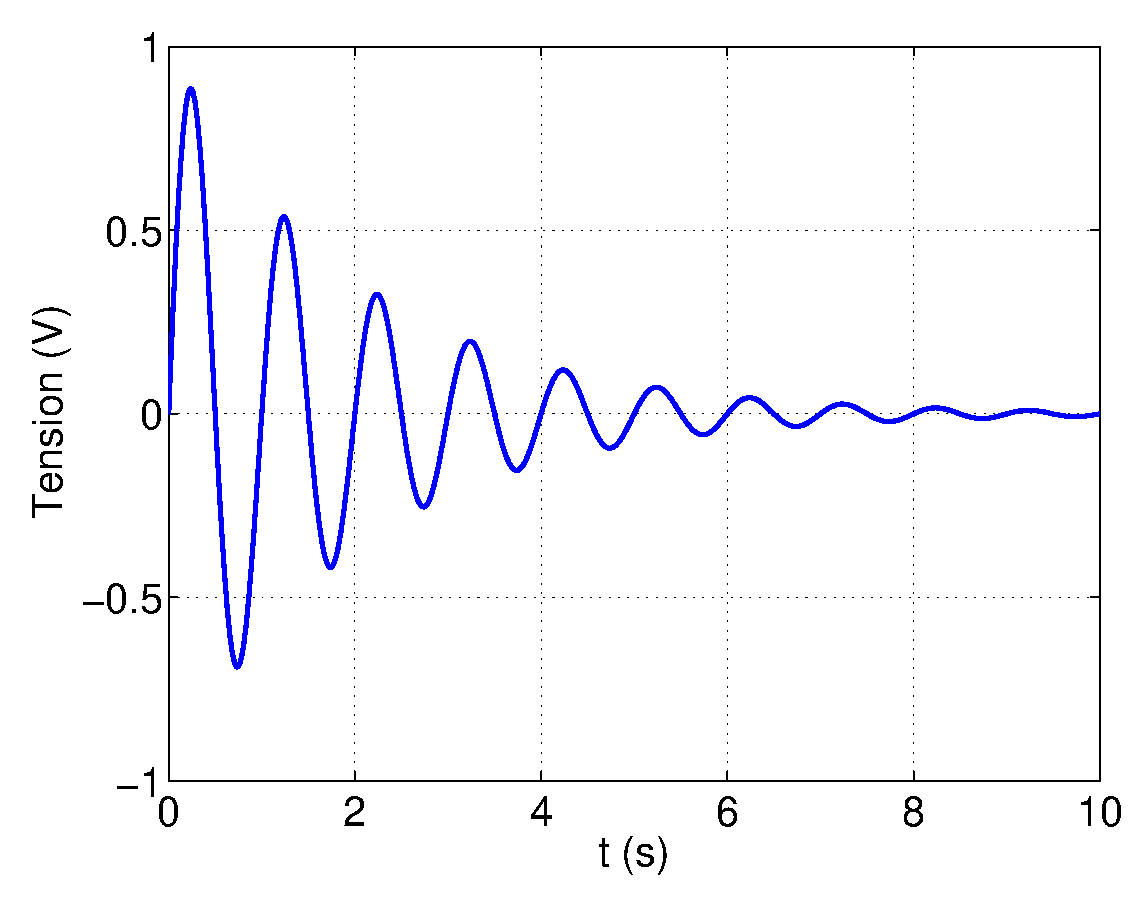
\includegraphics[height=2.4cm]{Figuras/UniScalar.eps}\\{\tiny $f(t)$}} & \parbox{3cm}{\centering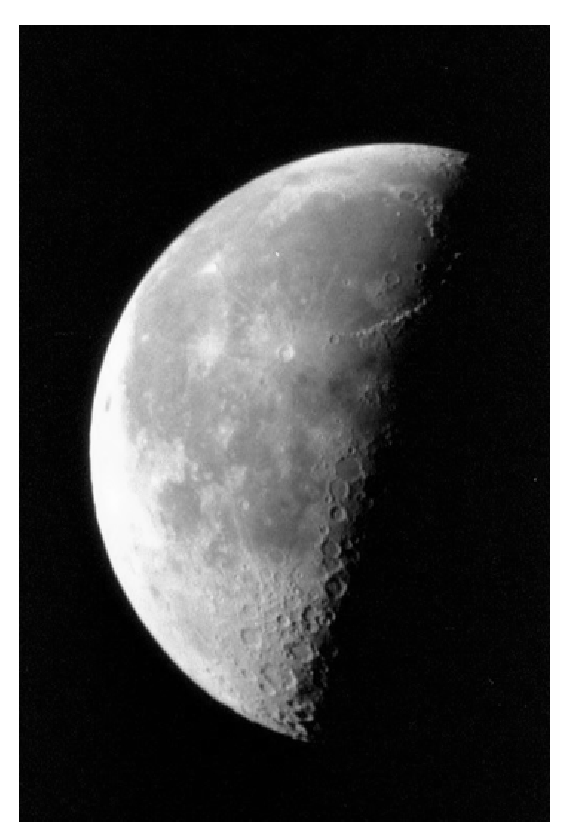
\includegraphics[height=2.3cm]{Figuras/Figures/ImagenBW.eps}\\{\tiny$f(x, y)$}} \\\\
    \rotatebox{90}{\color{red}\small Vectorial\color{black}}   & \parbox{4cm}{\centering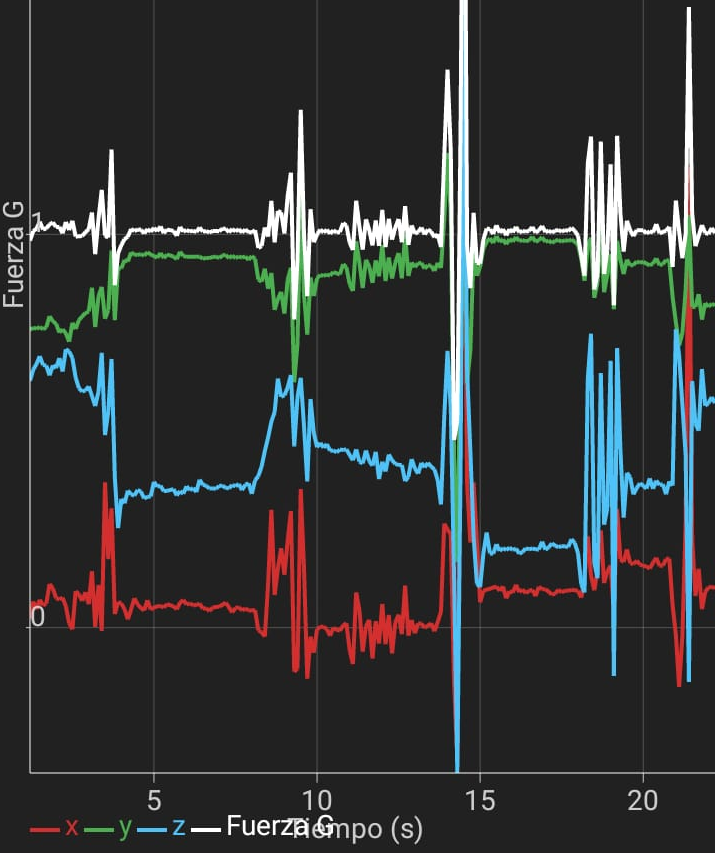
\includegraphics[width=2.0cm]{Figuras/UniVectorial.png}\\{\tiny$[f_x(t)~f_y(t)~f_z(t)~f_g(t)]$}} & \parbox{4cm}{\centering\includegraphics[height=2.3cm]{Figuras/Figures/ImagenColor.eps}\\{\tiny$[f_R(x, y)~f_G(x, y)~f_B(x, y)]$}} \\
  \end{tabular}
\end{frame}

% Basado en la presentación, aquí tienes ejemplos prácticos para 
% cada uno de los tipos de señales mencionados:

% 1. Según el número de fuentes o variables (Tipos I)
% Unidimensional: 


% Una señal de audio (voz), donde la presión acústica varía solo 

% en función del tiempo1111.


% Multidimensional: Una fotografía digital (imagen fija), que 
% varía en función de dos variables espaciales $(x, y)$

% 2222.Escalar: 
% La medición de la temperatura de una habitación a
%  lo largo del día3.
 
%  Vectorial: Una señal de vídeo en color (RGB),
 
%  donde en cada punto y momento se tienen tres componentes de 
%  intensidad (Rojo, Verde y Azul)
 
%  4444.2. 
%  Según la naturaleza de la variable y la amplitud (Tipos II)A
%  nalógica (Continua en tiempo y amplitud): 
%  La tensión eléctrica que sale directamente de un micrófono 
%  antes de ser procesada
 
%  5555.Muestreada (Discreta en tiempo, continua en amplitud): 
%  Los valores de esa tensión tomados a intervalos regulares, 
%  pero manteniendo su precisión decimal exacta antes de ser 
%  convertidos a bits
 
%  6.Digital (Discreta en tiempo y amplitud): 
%  Un archivo MP3 o un audio grabado en un CD, 
%  donde los valores ya están cuantizados en niveles definidos 
%  (bits)
%  7.3. 
 
%  Según su determinación (Tipos III)Determinista: Una señal de reloj de un procesador o un tono puro generado por un sintetizador ($x[n] = \sin(n)$), cuyo valor futuro es predecible8.Aleatoria / Estocástica: El ruido blanco (estática) de una radio sin sintonizar o las fluctuaciones del mercado de valores, que solo pueden describirse mediante probabilidades9.4. Según su repetición y simetría (Tipos IV y V)Periódica: La señal de la red eléctrica (50Hz/60Hz), que repite su forma de onda senoidal constantemente10.Aperiódica: Un golpe de tambor único o una palabra suelta, que no se repiten de forma infinita11.Par: Una señal de pulso rectangular centrado en el origen $t=0$12121212.Impar: Una señal de onda senoidal $(\sin(t))$, que es simétrica respecto al origen13131313.5. Según su relación con el tiempo (Tipos VI)Causal: Cualquier sistema físico real en funcionamiento, como un sensor que empieza a registrar datos solo después de encenderse (vale 0 para $t < 0$)14.Anticausal: Se utiliza principalmente en procesado de archivos grabados (post-procesamiento), donde podemos analizar la señal "hacia atrás" desde el presente hacia el pasado15.6. Según su energía y potencia (Tipos VII y VIII)De Energía Finita: Un pulso único o un transitorio que desaparece rápidamente; tiene una duración limitada16.De Potencia Finita: Una onda senoidal infinita o el ruido constante de un motor; aunque duran para siempre, su promedio de energía por unidad de tiempo es constante17.7. Señales Básicas de la PresentaciónImpulso ($\delta$ de Dirac): El modelo matemático de un martillazo instantáneo o un destello de flash fotográfico18.Escalón ($u(t)$): El acto de encender un interruptor, donde la tensión pasa de 0 a un valor constante instantáneamente19.Chirp: El sonido que emiten los radares o los delfines, cuya frecuencia aumenta o disminuye con el tiempo20.





\begin{frame}
  \frametitle{Tipos de señales II}
  \vspace{-0.1cm}
  \begin{itemize}
    \item <1-> Respecto a la variable independiente:
    \begin{itemize}
      \vspace{0.1cm}
      \item \alert{Continua}: $x(t)$ con $t\in \mathbb{R} $ (real)
      \vspace{0.1cm}
      \item \alert{Discreta}: $x(n)$ (o secuencia x[n]) con $n\in \mathbb{Z}$ (entero)
    \end{itemize}
    \vspace{0.2cm}
    \item <2-> Respecto a la amplitud $x(\cdot)$ de la señal:
    \begin{columns}[T]
      \visible<1->{\begin{column}{4.6cm}
      \begin{itemize}
        \vspace{0.0cm}
        \item $x(\cdot) \in \mathbb{R}$  \color{gray}{(a $x(\cdot) \in \mathbb{C}$)}\color{black}
        \begin{itemize}
          \vspace{0.1cm}
          \item  $x(t) \rightarrow$ \alert{Analógica}
          \vspace{0.1cm}
          \item $x[n] \rightarrow$ \alert{Muestreada}
        \end{itemize}
        \vspace{0.2cm}
        \item  $x(\cdot) \in S$ discreto:
        \begin{itemize}
          \vspace{0.1cm}
          \item  $x(t) \rightarrow$ \alert{Cuantizada}
          \vspace{0.1cm}
          \item $x[n] \rightarrow$ \alert{Digital}
        \end{itemize}
        \vspace{0.1cm}
        \color{gray} { Ej: $ S\!=\! \{\!a\!+\!b\!\cdot \!k | k \!\in \! \mathbb{Z}\}$}
      \end{itemize}
    \end{column}}
    \hspace{-0.5cm} \visible<1->{\begin{column}{6cm}
    \begin{figure}
      \centering
      \footnotesize
      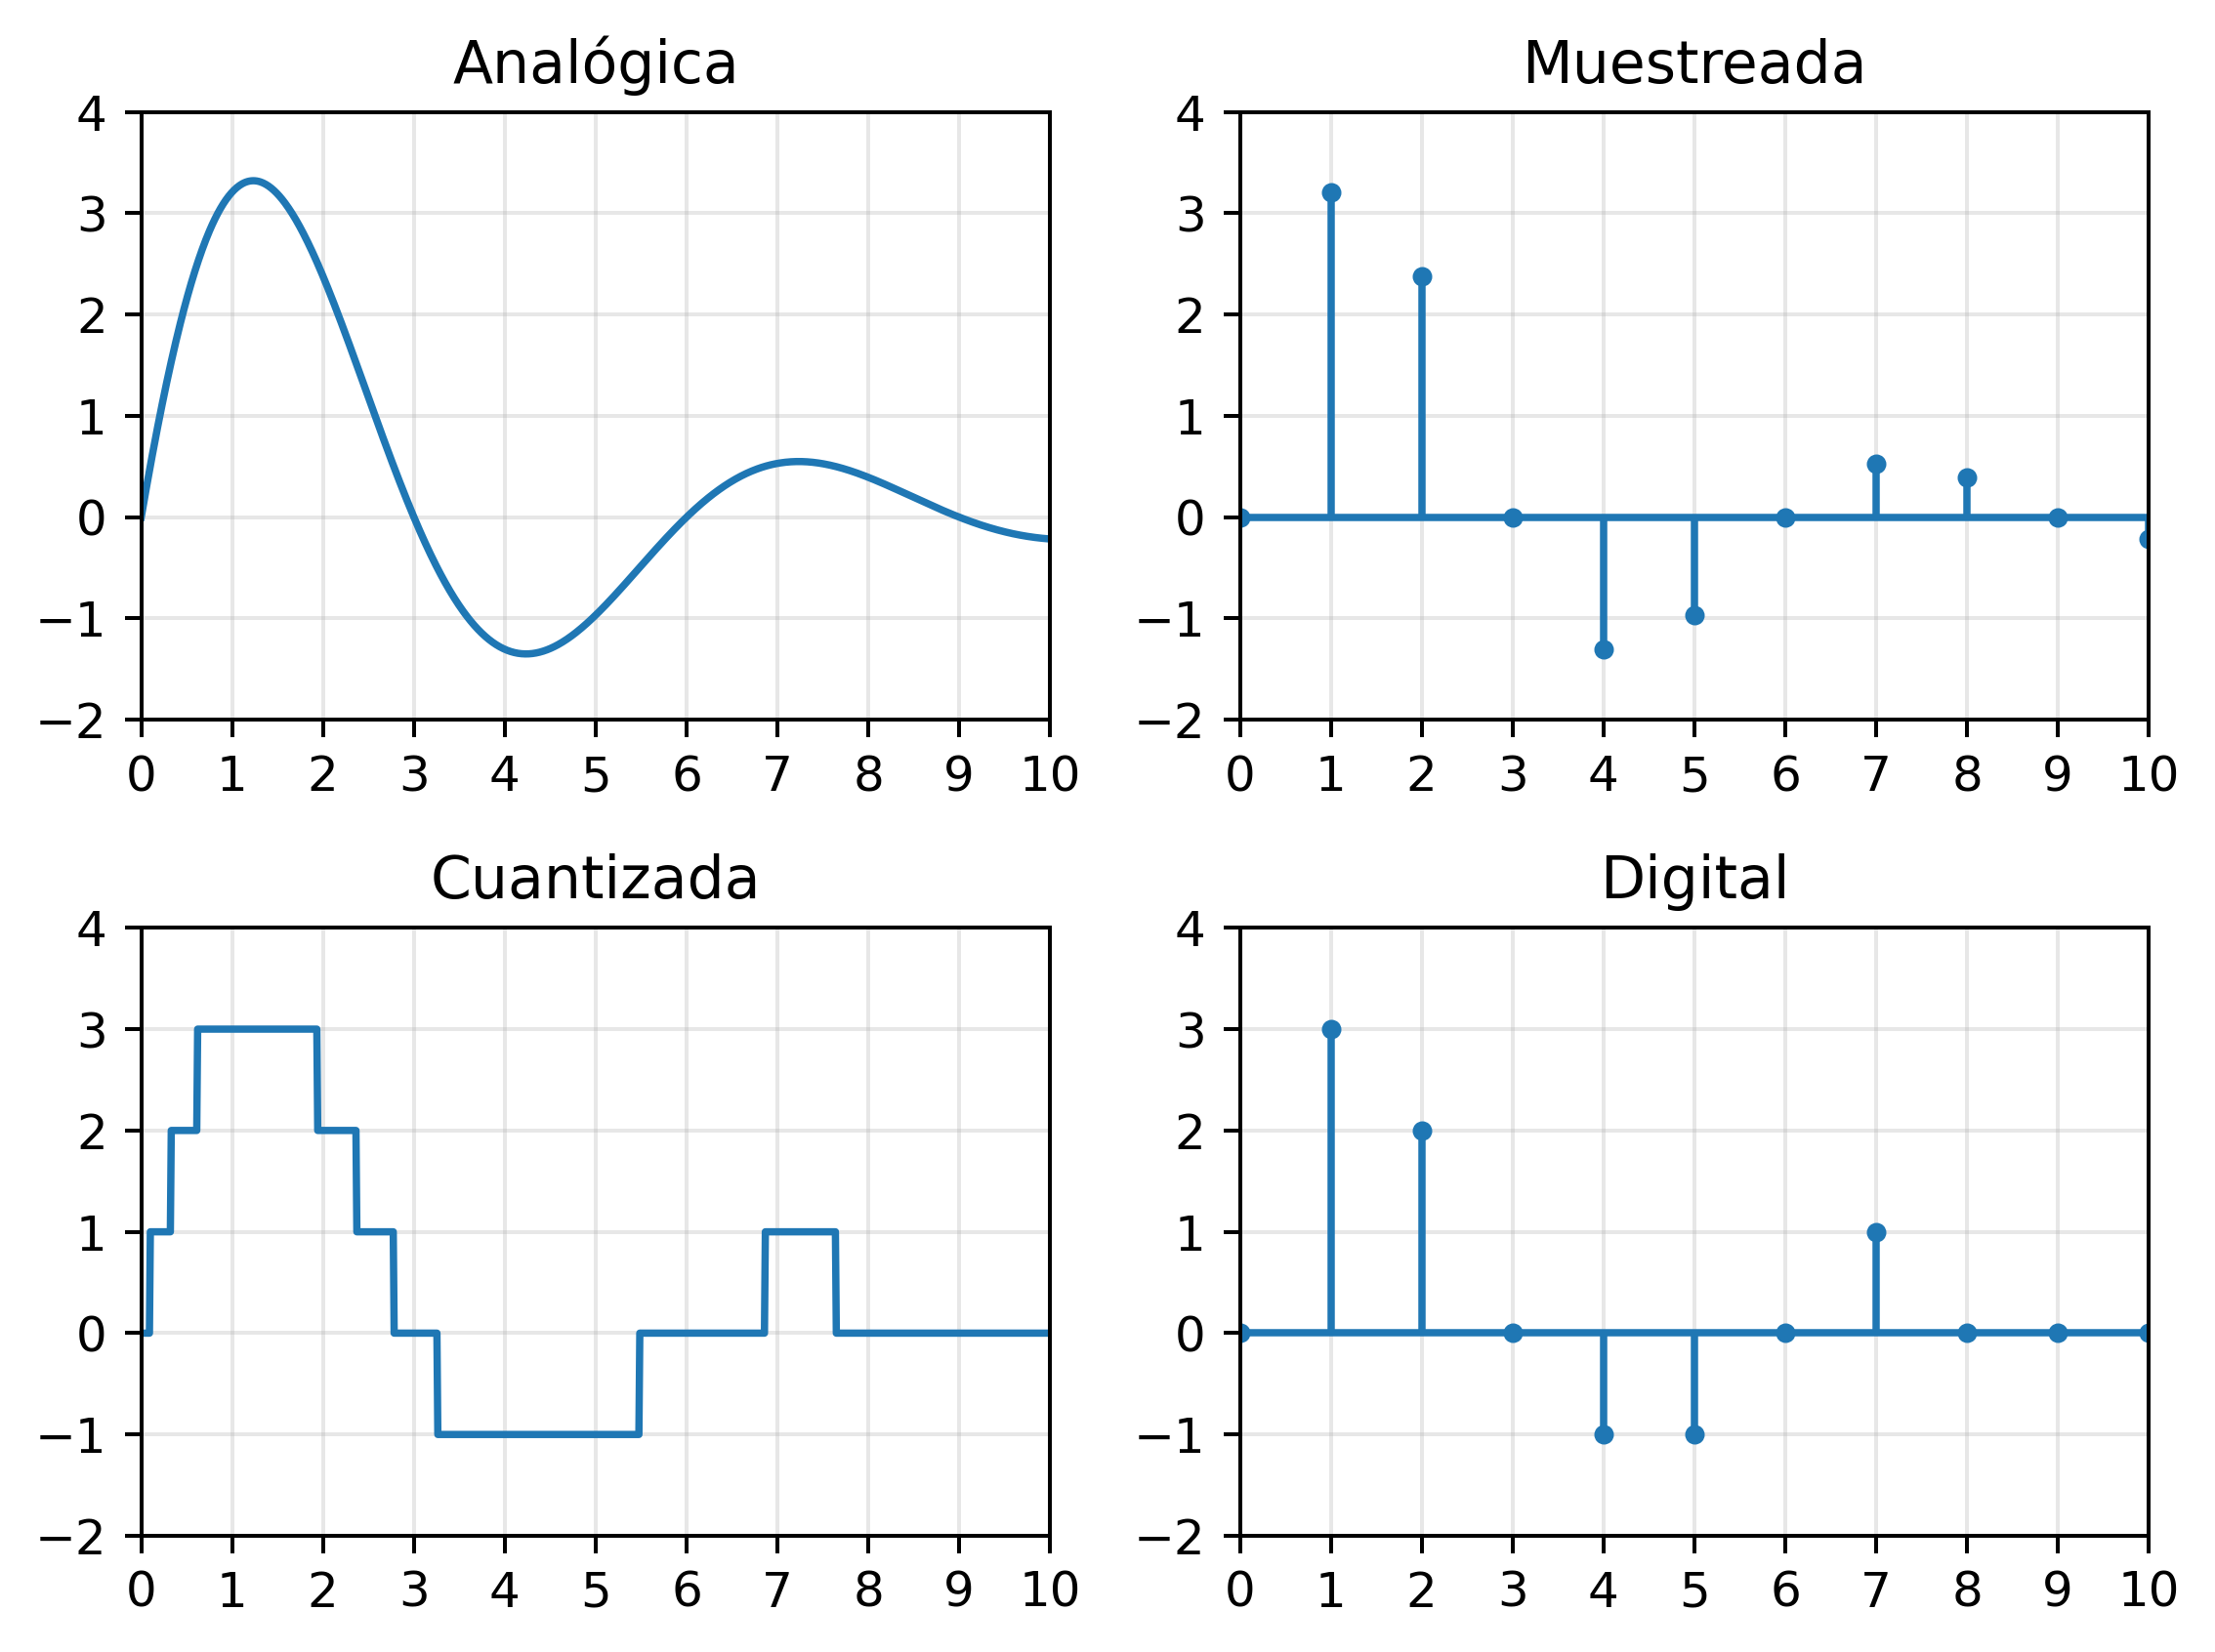
\includegraphics[width=6cm]{Figuras/ad.png}
    \end{figure}
    \end{column}}
  \end{columns}
  \end{itemize}
  \vspace{-0.5cm}
\end{frame}


\begin{frame}
  \frametitle{Tipos de señales III}
  \vspace{-0.1cm}
  \begin{itemize}
    \item <1-> Evolución de la señal (valor en cada instante de tiempo):
    \begin{itemize}
      \vspace{0.1cm}
      \item \alert{Determinista}:  está definido por una expresión matemática
      \vspace{0.1cm}
      \item \alert{Aleatoria/Estocástica}:  queda definido por una densidad de probabilidad (no se puede determinar de forma exacta).
    \end{itemize}
  \end{itemize}
  \vspace{-0.3cm}
  \begin{figure}
    \centering
    \footnotesize
    \begin{tabular}{@{\extracolsep{-8pt}}cc}
      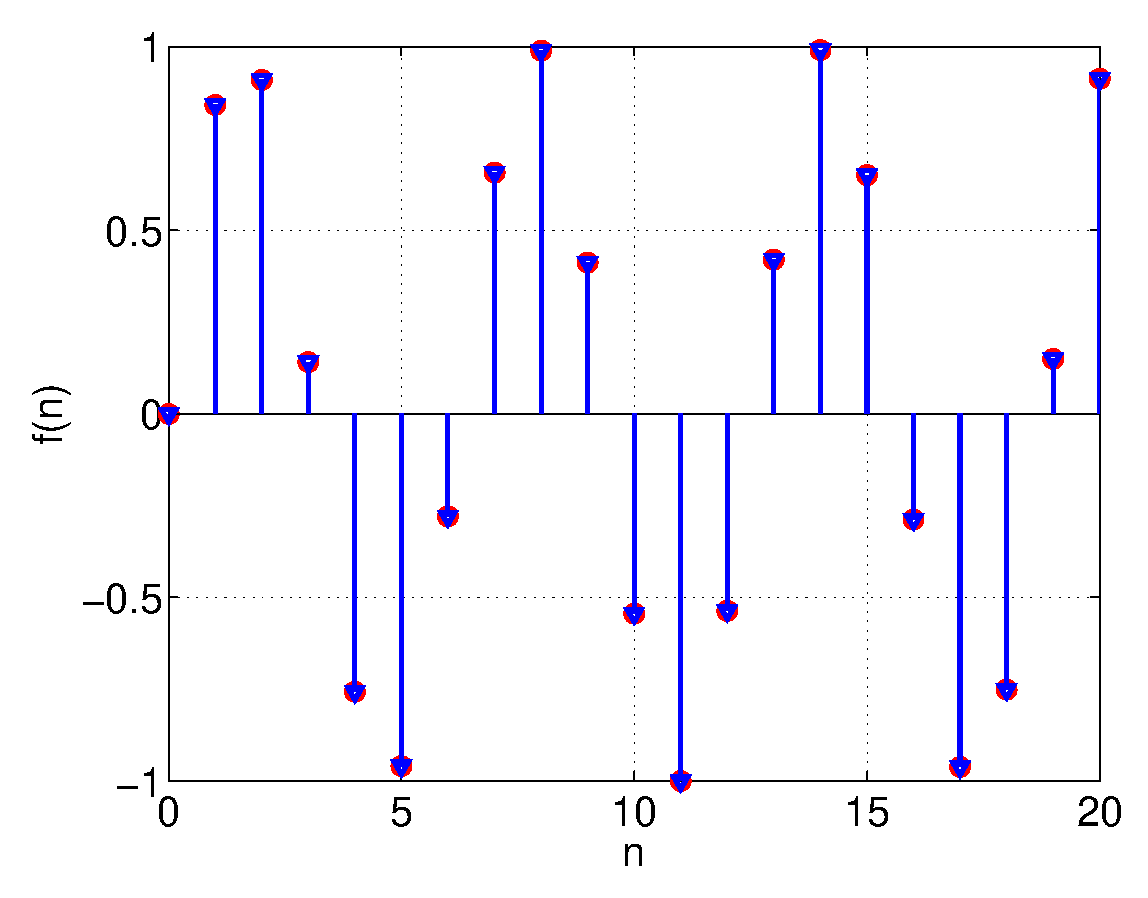
\includegraphics[width=5cm]{./Figuras/Determinista.eps}&
      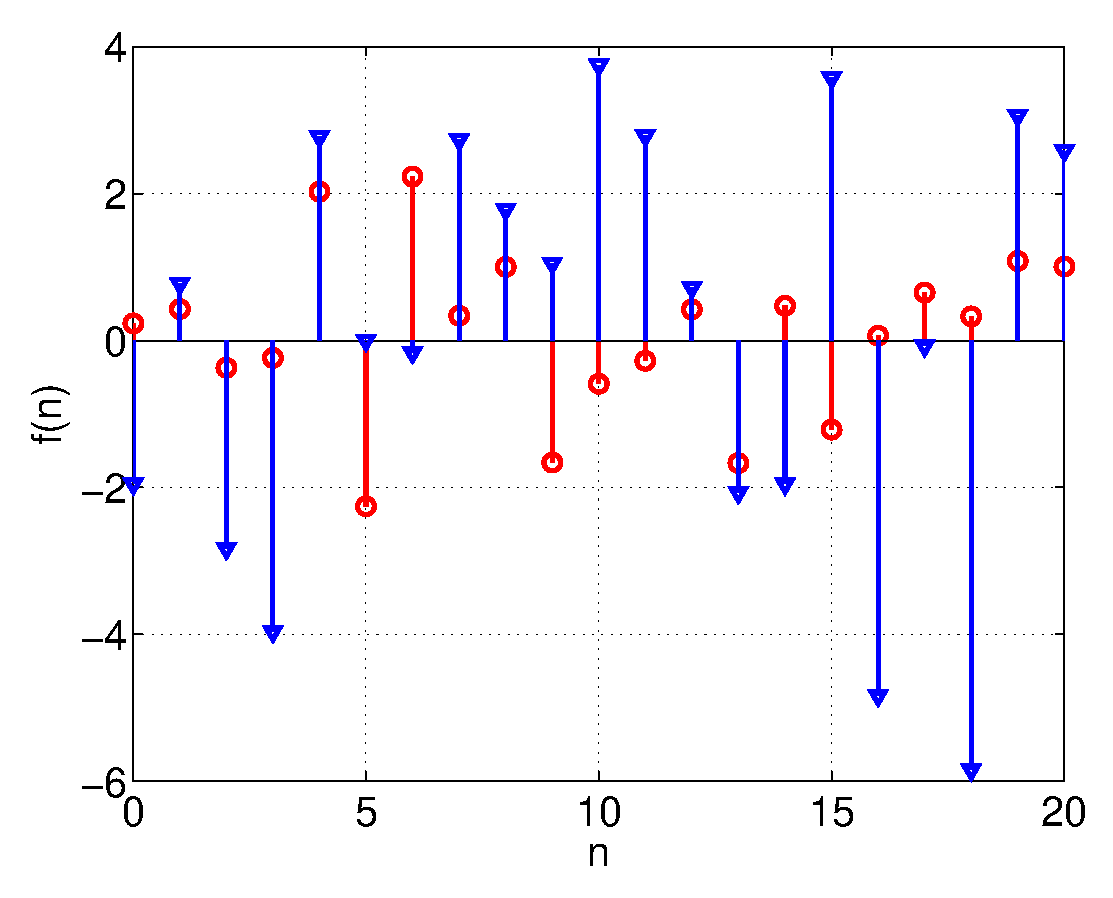
\includegraphics[width=5cm]{./Figuras/Aleatorio.eps}\\
      Determinista  & Aleatoria \\
      $x[n]=sin(n)$ & $x[n] \sim \mathcal{N}(0,1) $
    \end{tabular}
  \end{figure}
\end{frame}

\begin{frame}
  \frametitle{Tipos de señales IV}
  \vspace{-0.1cm}
  \begin{itemize}
    \item <1-> Señales periódicas/aperiódicas:
    \begin{itemize}
      \vspace{0.1cm}
      \item \alert{Periódica}: su valor se repite en el tiempo, por lo tanto es suficiente especificar su valor a lo largo de un intervalo básico llamado periodo fundamental ($T$ o $N$).
      \begin{itemize}
        \vspace{0.1cm}
        \item Continua: $x(t+l\cdot T)=x(t)$
        \vspace{0.1cm}
        \item  Discreta: $x[n+l\cdot N]=x[n]$
        \vspace{0.1cm}
        con $l \in \mathbb{Z}^+$,  $N \in \mathbb{Z}^+$
      \end{itemize}
      \vspace{0.1cm}
      \item \alert{Aperiódica}:  no cumple la relación anterior.
    \end{itemize}
  \end{itemize}
  \vspace{-0.3cm}
  \begin{figure}
    \centering
    \footnotesize
    \begin{tabular}{@{\extracolsep{-8pt}}cc}
      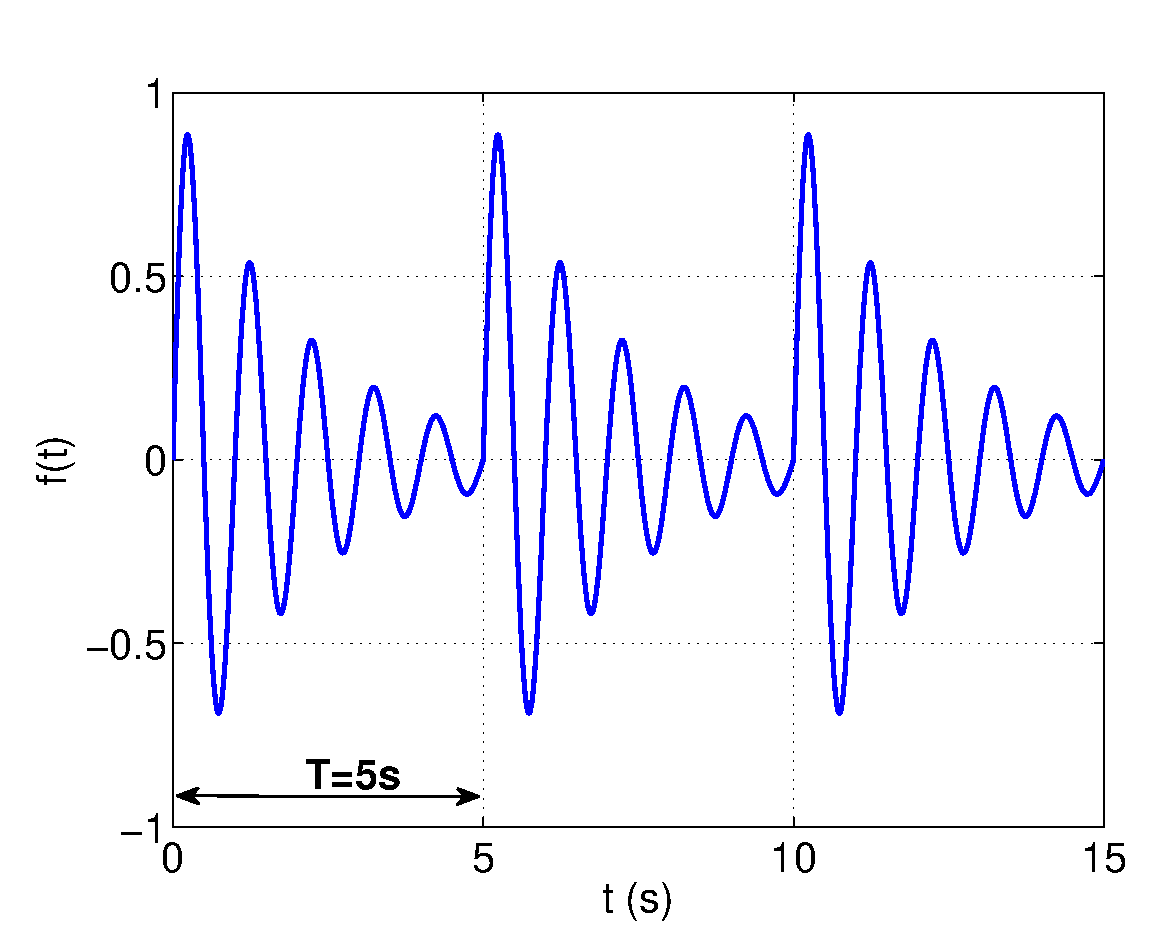
\includegraphics[width=5cm]{./Figuras/PeriodT.eps}&
      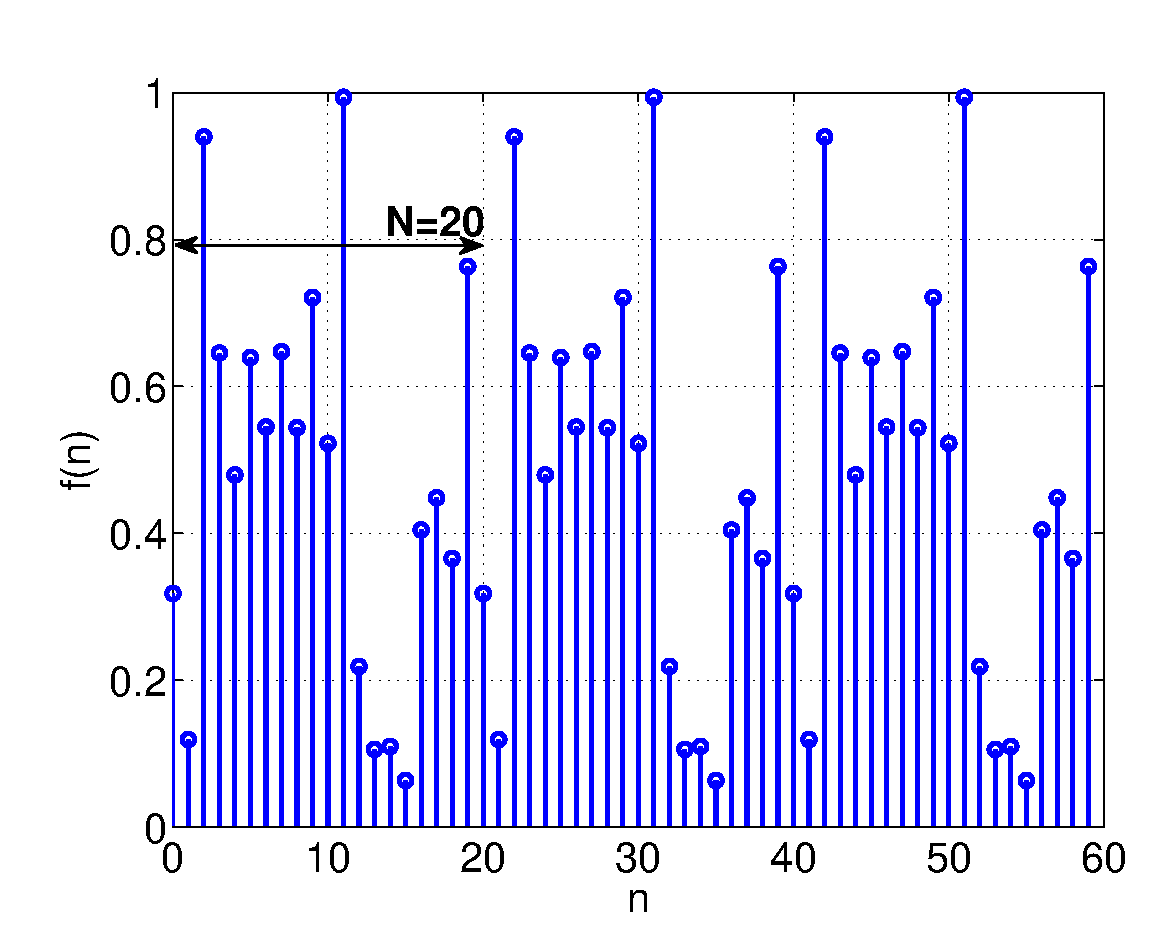
\includegraphics[width=5cm]{./Figuras/PeriodN.eps}\\
    \end{tabular}
  \end{figure}
\end{frame}

\begin{frame}
  \frametitle{Tipos de señales V}
  \vspace{-0.2cm}
  \begin{itemize}
    \item <1-> Señales pares/impares:
    \begin{itemize}
      \vspace{0.1cm}
      \item \alert{Par}: presenta simetría especular respecto a eje vertical.
      \vspace{0.1cm}
      \begin{itemize}
        \begin{columns}[c]
          \hspace{1cm}\begin{column}{3.8cm}
          \vspace{-0.15cm}
          \item Continua: $x(t)=x(-t)$
          \end{column}
          \hspace{-1.5cm}\begin{column}{3.8cm}
          \item  Discreta: $x[n]=x[-n]$
        \end{column}
      \end{columns}
    \end{itemize}
    \vspace{0.1cm}
    \item \alert{Impar}: presenta simetría radial respecto al origen.
    \vspace{0.1cm}
    \begin{itemize}
      \begin{columns}[c]
        \hspace{1cm}\begin{column}{3.8cm}
          \vspace{-0.15cm}
          \item Continua: $x(t)=-x(-t)$
        \end{column}
        \hspace{-1.5cm}\begin{column}{3.8cm}
          \item  Discreta: $x[n]=-x[-n]$
        \end{column}
      \end{columns}
    \end{itemize}
    \vspace{0.1cm}
    \vspace{0.1cm}
    \end{itemize}
  \end{itemize}
  \vspace{-0.75cm}
  \begin{figure}
    \centering
    \footnotesize
    \begin{tabular}{@{\extracolsep{-8pt}}cc}
      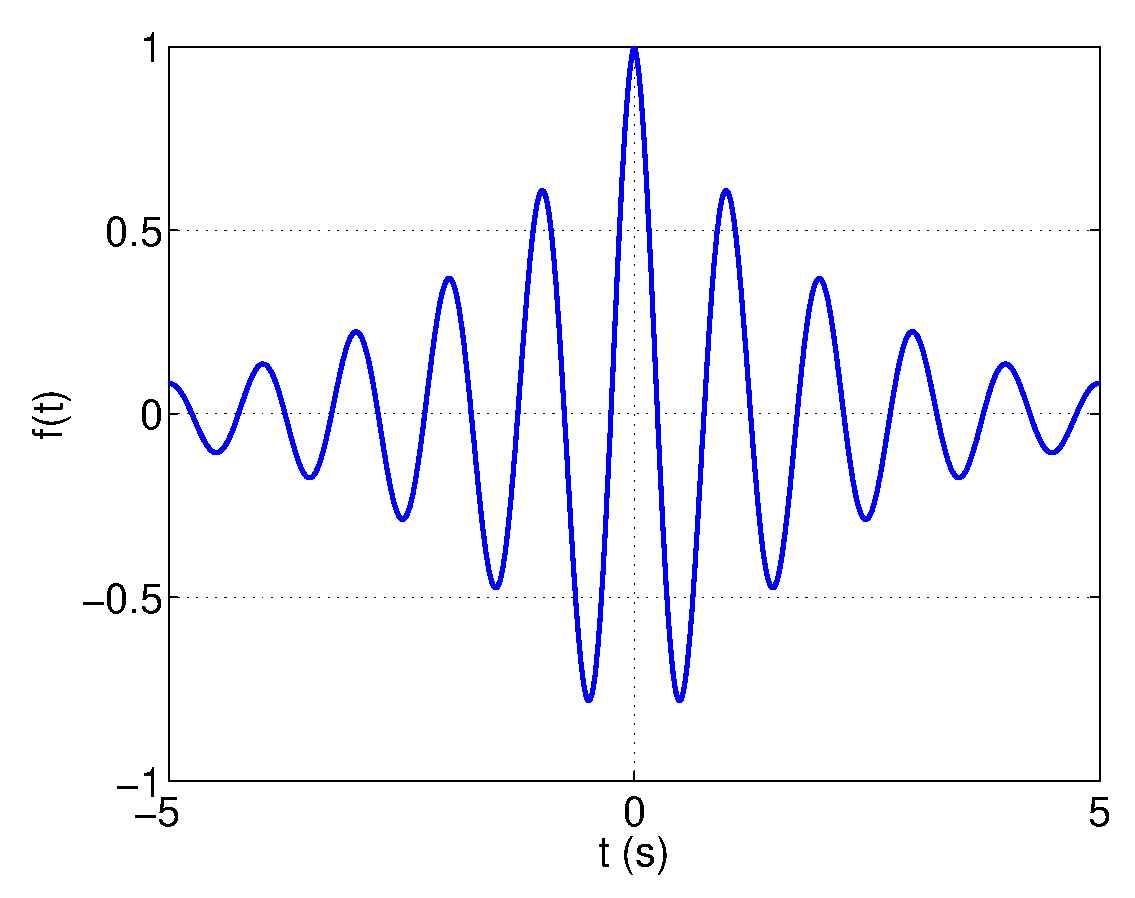
\includegraphics[width=4cm]{./Figuras/Par.eps}&
      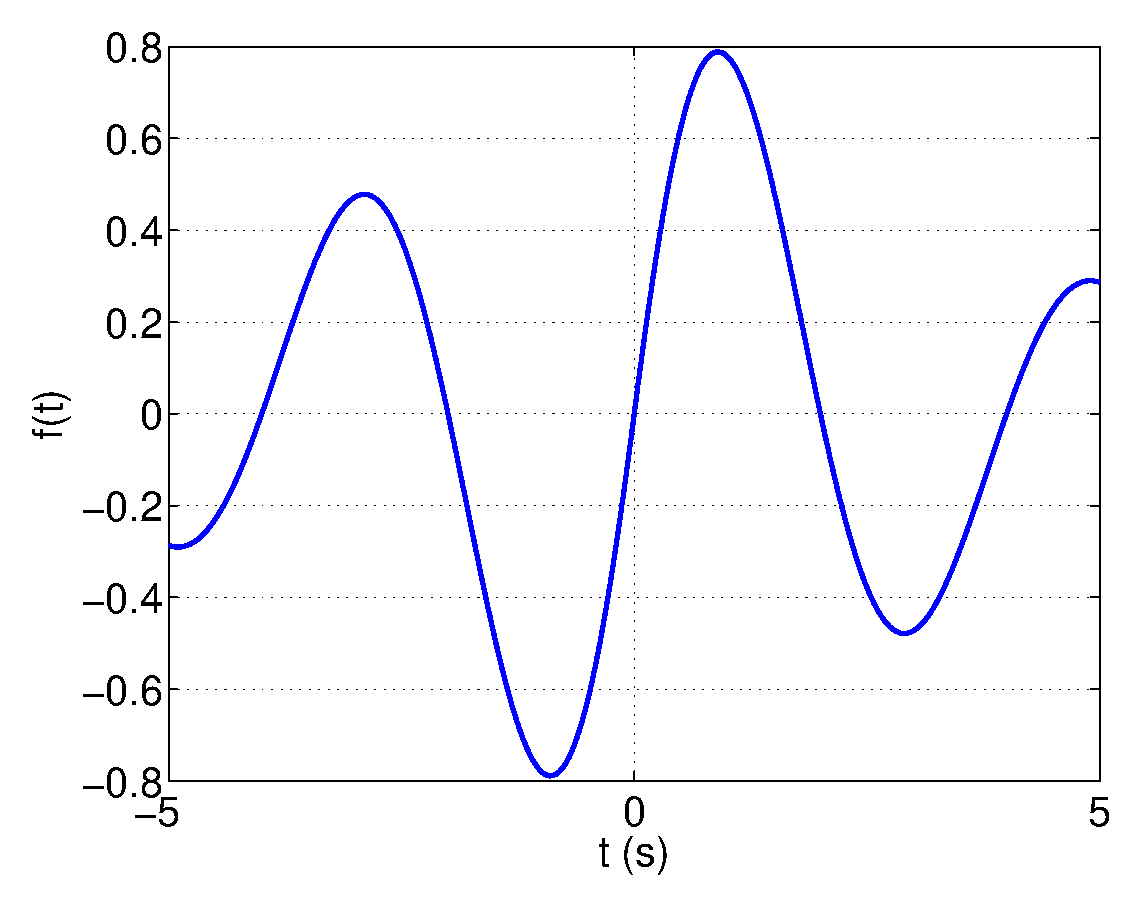
\includegraphics[width=4cm]{./Figuras/Impar.eps}\\
      Par & Impar
    \end{tabular}
  \end{figure}
  \vspace{-0.3cm}
  \footnotesize
  En general, una función arbitraria se puede descomponer en función de sus componentes par e impar:
$x(\cdot)=x_p(\cdot)+x_i(\cdot)$

  \vspace{+0.1cm}
  \hspace{3.6cm} $x_p(\cdot)=\frac{x(\cdot)+x(-\cdot)}{2}$,
  $x_i(\cdot)=\frac{x(\cdot)-x(-\cdot)}{2}$
\end{frame}

\begin{frame}
  \frametitle{Tipos de señales VI}
  \vspace{-0.1cm}
  \begin{itemize}
    \item <1-> Señales causales/no causales/anticausales:
    \begin{itemize}
      \vspace{0.1cm}
      \item \alert{Causal}: relacionadas con los sistemas realizables (causales).
      \begin{itemize}
        \begin{columns}[T]
          \hspace{1cm}\begin{column}{4cm}
            \vspace{0.0cm}
            \item Continua: $x(t)=0  \: \: \forall t<0$
          \end{column}
          \hspace{-1cm}\begin{column}{4cm}
            \vspace{0.1cm}
            \item  Discreta: $x[n]=0  \: \: \forall n<0$
          \end{column}
        \end{columns}
      \end{itemize}
      \vspace{0.1cm}
      \item \alert{No causal}:
      \begin{itemize}
        \begin{columns}[T]
          \hspace{1cm}\begin{column}{4cm}
            \vspace{0.0cm}
            \item Continua: $x(t)\neq 0  \: \: \exists t<0$
          \end{column}
          \hspace{-1cm}\begin{column}{4cm}
            \vspace{0.1cm}
            \item  Discreta: $x[n] \neq 0  \: \: \exists n<0$
          \end{column}
        \end{columns}
      \end{itemize}
      \vspace{0.1cm}
      \item \alert{Anticausal}:
      \begin{itemize}
        \begin{columns}[T]
          \hspace{1cm}\begin{column}{4cm}
            \vspace{0.0cm}
            \item Continua: $x(t)= 0  \: \:  \forall t>0$
          \end{column}
          \hspace{-1cm}\begin{column}{4cm}
            \vspace{0.1cm}
            \item  Discreta: $x[n]= 0  \: \: \forall n>0$
          \end{column}
        \end{columns}
      \end{itemize}
    \end{itemize}
  \end{itemize}
  \vspace{-0.3cm}
  \begin{figure}
    \centering
    \footnotesize
    \begin{tabular}{@{\extracolsep{-8pt}}ccc}
      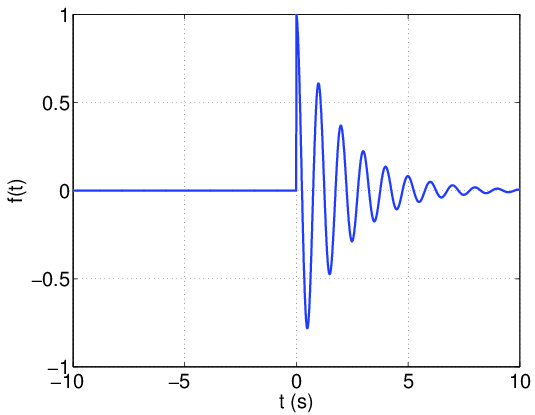
\includegraphics[width=3.7cm]{./Figuras/Causal}&
      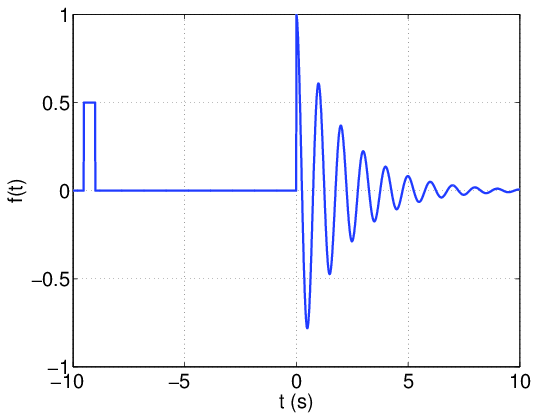
\includegraphics[width=3.7cm]{./Figuras/NoCausal}&
      \includegraphics[width=3.7cm]{./Figuras/Anticausal}\\
      Causal & No causal & Anticausal
    \end{tabular}
  \end{figure}
\end{frame}

\begin{frame}
  \frametitle{Tipos de señales VII}
  \begin{itemize}
    \item <1-> Señales definidas en energía):
    \begin{itemize}
      \vspace{0.2cm}
      \item \alert{Energía de una señal}:
      \vspace{0.2cm}
      \begin{itemize}
        \item Continua: $\varepsilon_x=\int^\infty_{-\infty}|x(t)|^2 dt $
        \vspace{0.2cm}
        \item  Discreta: $\varepsilon_x=\sum^{\infty}_{n=-\infty}|x[n]|^2 $
      \end{itemize}
      \vspace{0.2cm}
      \item \alert{Señal de energía finita}:  $0<\varepsilon_x<\infty$
      \begin{itemize}
        \vspace{0.2cm}
        \item En general son señales limitadas en el tiempo con amplitud finita
        \item Se puede analizar su espectro con la Transformada de Fourier.
      \end{itemize}
      \vspace{-0.2cm}
    \end{itemize}
  \end{itemize}

  \begin{figure}
    \centering
    \footnotesize
    \begin{tabular}{@{\extracolsep{-8pt}}cc}
      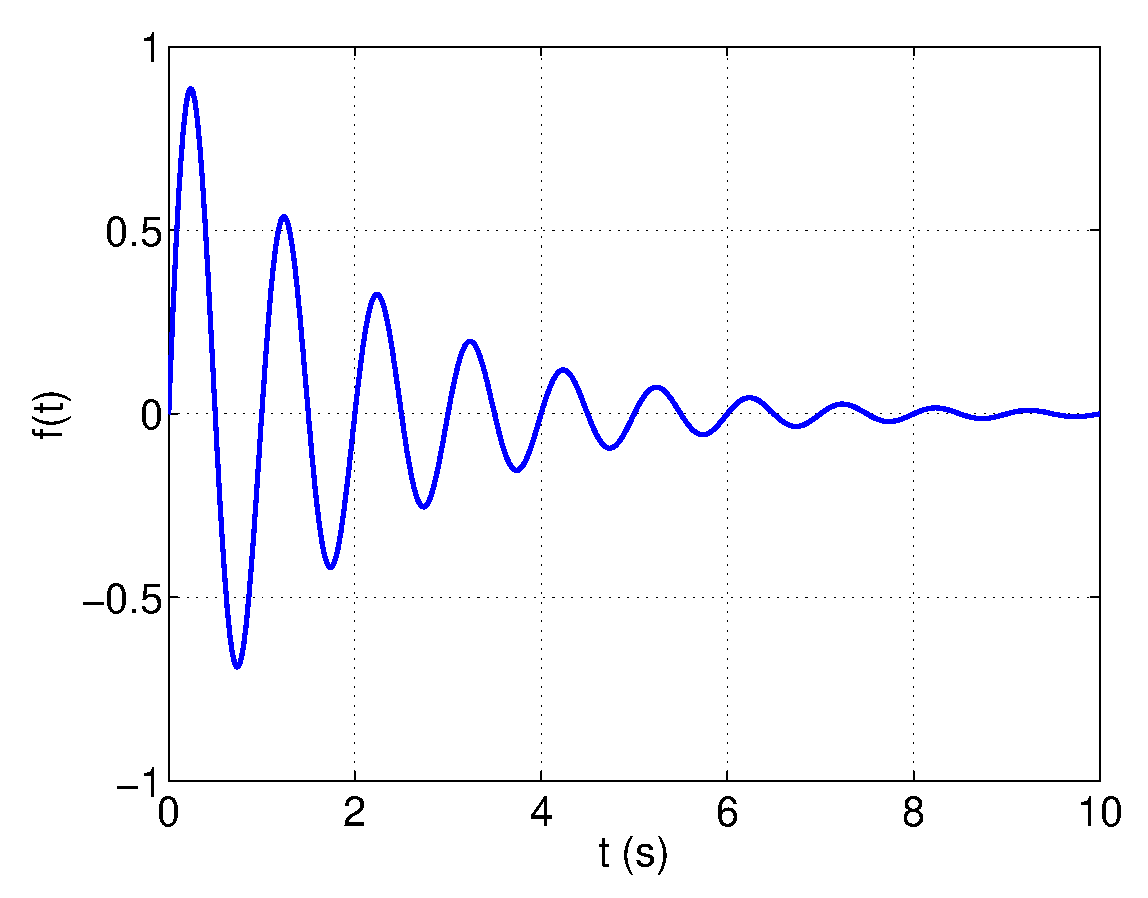
\includegraphics[width=4.5cm]{./Figuras/EnergiaF.eps}&
      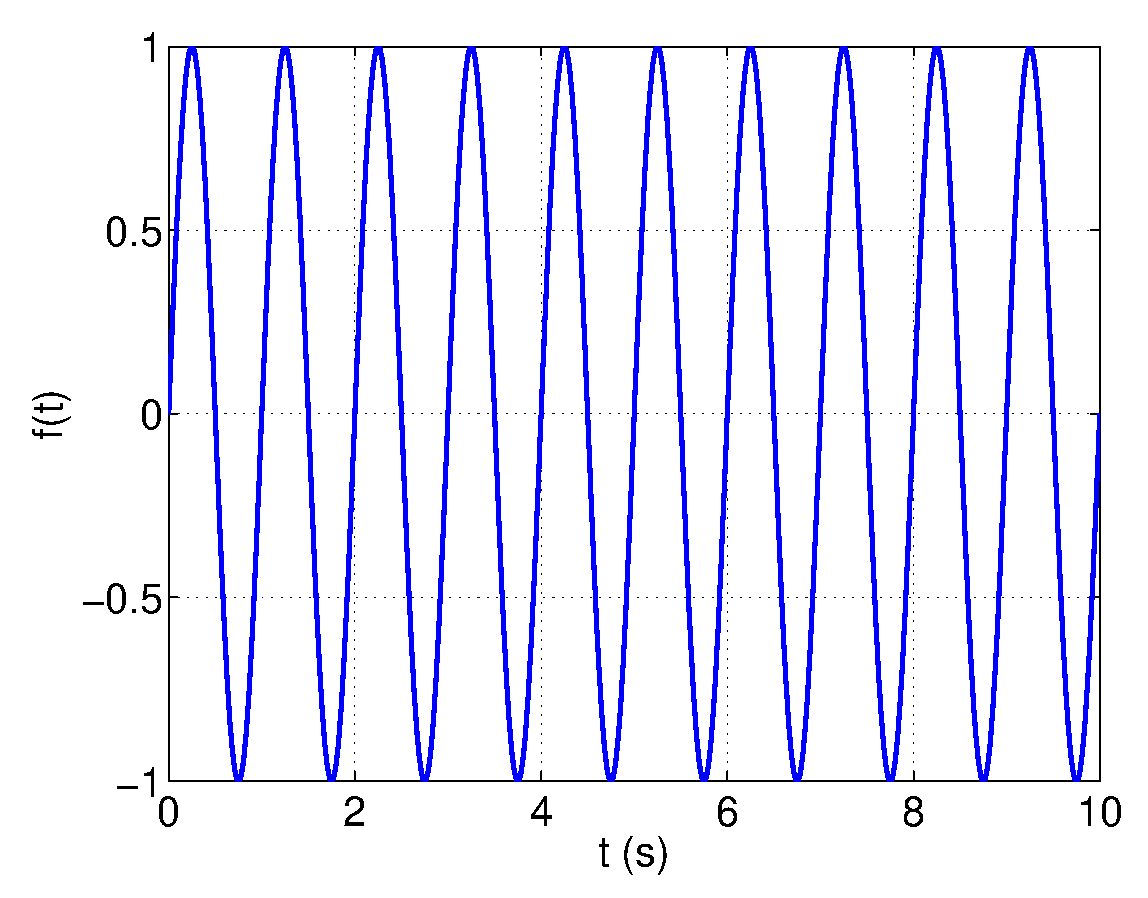
\includegraphics[width=4.5cm]{./Figuras/EnergiaI.eps}\\
      Energía finita & Energía infinita
    \end{tabular}
  \end{figure}
\end{frame}

\begin{frame}
  \frametitle{Tipos de señales VIII}
  \begin{itemize}
    \item <1-> Señales definidas en potencia:
    \begin{itemize}
      \vspace{0.2cm}
      \item \alert{Potencia media de una señal}:
      \vspace{0.2cm}
      \begin{itemize}
        \item Continua: $P_f=\lim_{T\rightarrow \infty} \frac{1}{T} \int^T_{-T}|x(t)|^2 dt $
        \vspace{0.2cm}
        \item  Discreta: $P_f=\lim_{N\rightarrow \infty} \frac{1}{2N+1}\sum^{N}_{n=-N}|x[n]|^2 $
      \end{itemize}
      \vspace{0.2cm}
      \item \alert{Señal de potencia media finita}:  $0<P_f<\infty$
      \begin{itemize}
        \vspace{0.2cm}
        \item En general son señales ilimitadas en el tiempo con amplitud finita.
      \end{itemize}
      \vspace{-0.4cm}
    \end{itemize}
  \end{itemize}

  \begin{figure}
    \centering
    \footnotesize
    \begin{tabular}{@{\extracolsep{-8pt}}cc}
      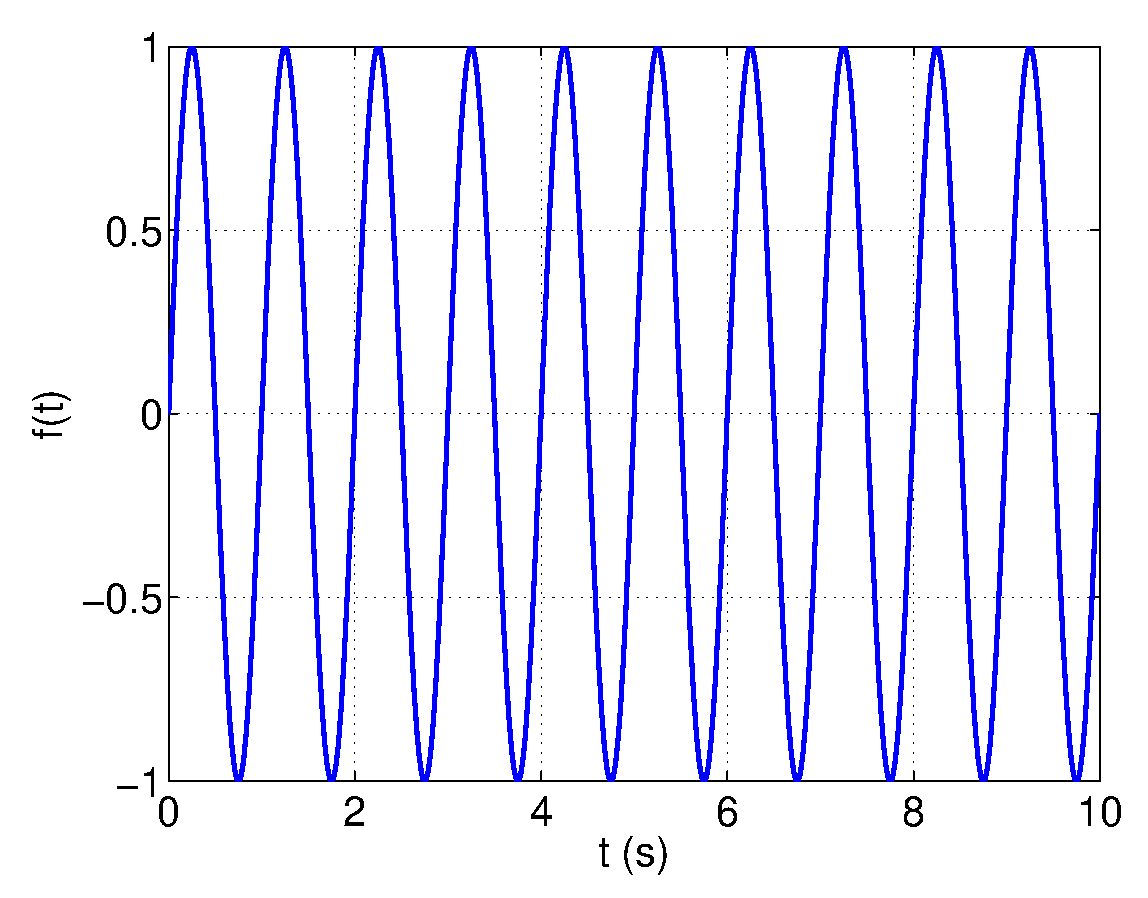
\includegraphics[width=4cm]{./Figuras/EnergiaI.eps}&
      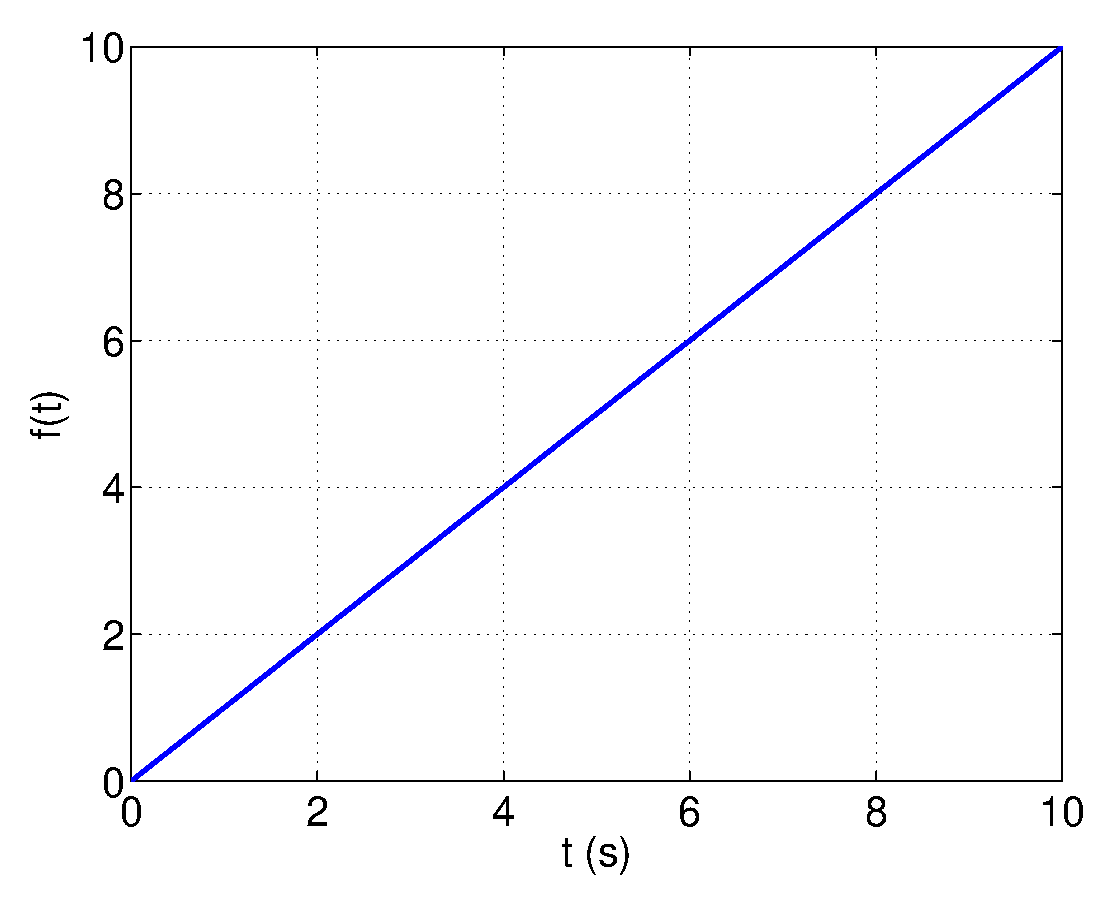
\includegraphics[width=3.8cm]{./Figuras/PotenciaI.eps}\\
      Potencia finita & Potencia infinita
    \end{tabular}
  \end{figure}

  \scriptsize \color{gray} \textit{Señales que no son de energía ni de potencia media finita son en general ilimitadas en el tiempo y/o amplitud.}
\end{frame}

% % %%%%%%%%%%%%%%%%%%%%%%%%%%%%%%%%%%%%%%%%%%%%%%%%%%%%%%

\begin{frame}
  \frametitle{Tipos de señales IX}
  \vspace{-0.1cm}
  \small
  \begin{itemize}
    \item \alert{Señal compleja}:  $x(\cdot) \in \mathbb{C}$
    \vspace{0.1cm}
    \begin{itemize}
      \footnotesize
      \item Se representa mediante dos funciones reales que contengan la parte real e imaginaria, o la fase y la amplitud\\ [1ex]
      \hspace{0.4cm}$x(\cdot)=\mathrm{Re}\{x(\cdot)\}+j \cdot \mathrm{Im}\{ x(\cdot)\}=|x(\cdot)| \mathrm{e}^{j \cdot \mathrm{arg} x(\cdot)}$
      \vspace{0.2cm}
      \begin{columns}[T]
        \begin{column}{4.75cm}
          \footnotesize\centering
          Parte real e imaginaria
          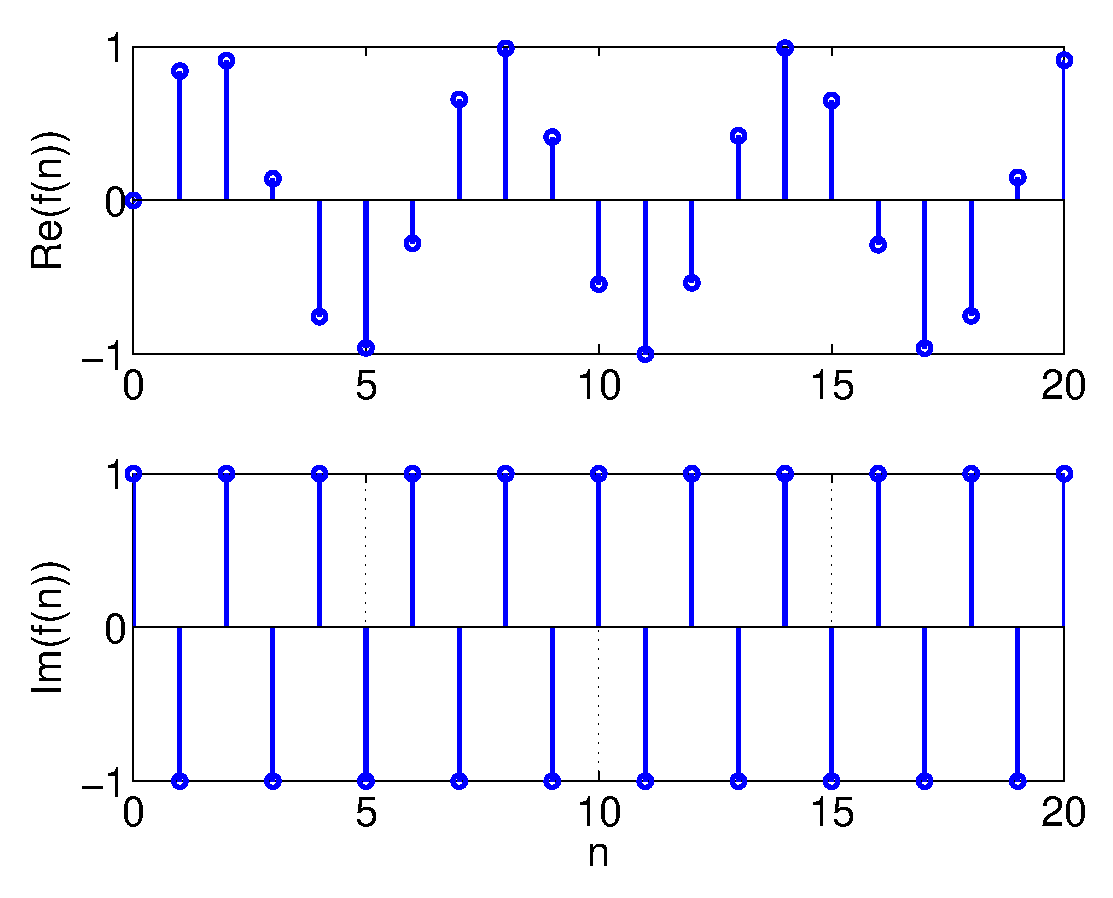
\includegraphics[width=3.5cm]{Figuras/ReIm.eps}
          $\begin{aligned}
            \mathrm{Re}(x(\cdot)) &= |x(\cdot)| \mathrm{cos}(\mathrm{arg}~x(\cdot) ) \\
            \mathrm{Im}(x(\cdot)) &= |x(\cdot)| \mathrm{sin}(\mathrm{arg}~x(\cdot))
          \end{aligned}$
        \end{column}
        \hspace{-1.2cm} \begin{column}{4.5cm}
          \footnotesize\centering
          Módulo y argumento
          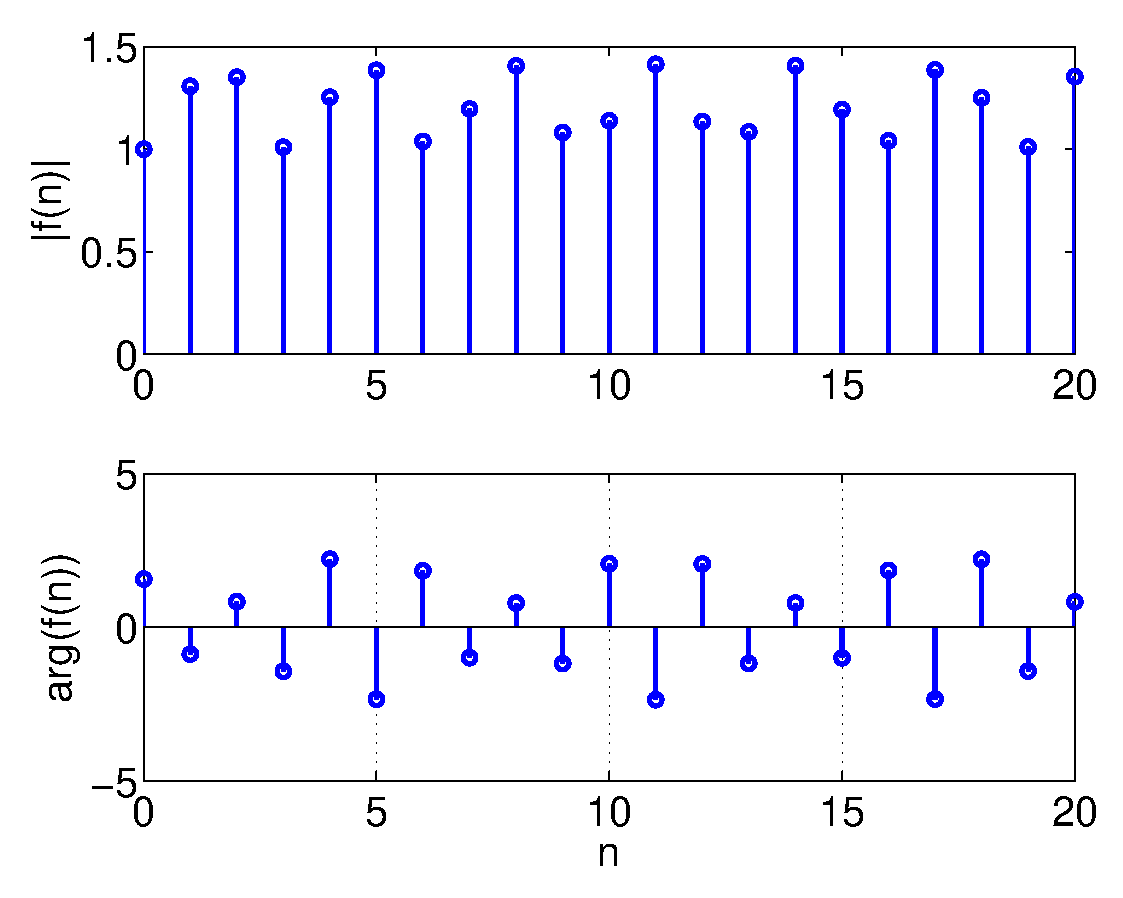
\includegraphics[width=3.5cm]{Figuras/ModArg.eps}\\
          $\begin{aligned}
            |x(\cdot)|            &= \sqrt{\mathrm{Re}\{x(\cdot)\}^2+\mathrm{Im}\{x(\cdot)\}^2} \\
            \mathrm{arg} x(\cdot) &= \arctan \frac{\mathrm{Im}\{x(\cdot)\}}{\mathrm{Re}\{x(\cdot)\}}
        \end{aligned}$
        \end{column}
      \end{columns}
    \end{itemize}
  \end{itemize}

  \vspace{-0.1cm}

  \scriptsize \color{gray} \textit{Series y Transformadas de Fourier. En teoría de la comunicación modelan señales  que transmiten información en fase y amplitud}

\end{frame}

% %%%%%%%%%%%%%

\begin{frame}
  \frametitle{Tipos de señales X}
  \vspace{-0.1cm}
  \small
  \begin{itemize}
    \item \alert{Señal reales}:$x(\cdot) = x^*(\cdot)$\\
    \vspace{0.1cm}
    \color{gray} $a(t)+j\cdot b(t)=a(t)-j \cdot b(t) \rightarrow b(t)=0$ \color{black}\\
    \item \alert{Señal imaginarias}: $x(\cdot) = -x^*(\cdot)$
    \vspace{0.1cm}
    \color{gray} $a(t)+j\cdot b(t)=-(a(t)-j \cdot b(t)) \rightarrow a(t)=0$ \color{black}\\
    \item \alert{Señal hermítica}:  $x(\cdot) = x^*(-\cdot)$
    \vspace{0.1cm}
    \color{gray} $a(t)+j\cdot b(t)=a(-t)-j \cdot b(-t) \rightarrow a(t)$ Par, $b(t)$ Impar \color{black}
    \item \alert{Señal antihermítica}: $x(\cdot) = -x^*(-\cdot)$\\
    \vspace{0.1cm}
    \color{gray} $a(t)+j\cdot b(t)=-(a(-t)-j \cdot b(-t)) \rightarrow a(t)$ Impar, $b(t)$ Par \color{black}
    \\ \vspace{0.2cm}
    con $^*$ conjugado.
  \end{itemize}

  \vspace{-0.3cm}
  \rule{10cm}{0.4pt}
  \vspace{0.2cm}\\
  \color{olivegreen}{Vamos a trabajar con señales: 1D (2D) escalares, continuas y discretas, analógicas y muestreadas, deterministas y aleatorias, periódicas y aperiódicas, reales y complejas.}

\end{frame}


%%%%%%%%%%%%%%%%%%%%%%%%%%%%%%%%%%%%%%%%%%%%%%

\begin{frame}
	\frametitle{Señales básicas: Impulso}
	
	\begin{itemize}
        \item \alert{Continuo ($\delta$ de Dirac):} {\scriptsize \hspace{1cm}$\delta(t)=\left \{ \begin{array}{l} \infty \:\: \: \:t=0\\0 \:\: \:\: \forall t \neq0\end{array}\right .$}%
        \begin{columns}[c]
            \begin{column}{0.2\textwidth}\centering
                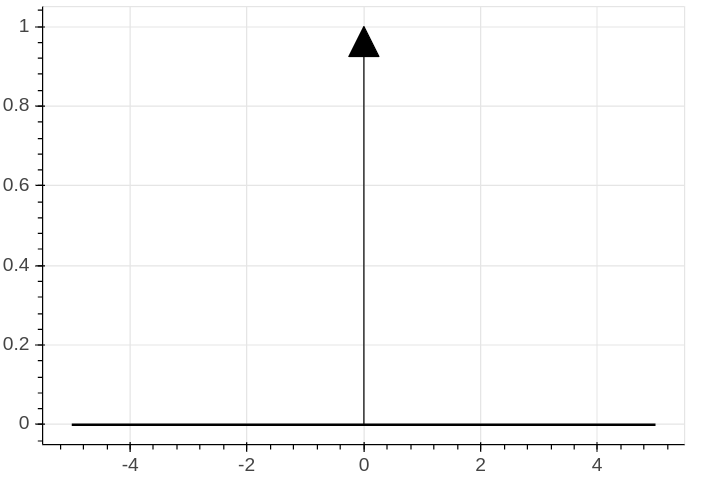
\includegraphics[width=4cm]{./Figuras/dirac}\\%
            \end{column}
            \hspace{0.3cm}
            \begin{column}{0.65\textwidth}
                {\scriptsize
                \begin{itemize}
                    {\scriptsize
                    \vspace{0.1cm}
                    \item Es un funcional:\\ \vspace{0.1cm}
                    $\int_{-\infty}^{\infty} f(t)\delta(t)dt=f(0)$\hspace{0.2cm}\color{olivegreen}$\int_{-\infty}^{\infty} f(t)\delta(t-t_0)dt=f(t_0)$\color{black}\\
                    \item Algunas propiedades:
                    $\int_{t_1}^{t_2} f(t)\delta(t-t_0)dt=\left\{\! \!\begin{array}{l}f(t_0)  \:\:\: t_1\!<t_0\!<t_2 \\ 0 \:\:\: c.c.    \end{array}\right .$
                    $\forall a\neq 0 \Rightarrow \delta(at)=\frac{\delta(t)}{|a|}$
                    $(x \ast \delta)(t) = \int_{-\infty}^\infty x(\tau)\delta(t-\tau)d\tau=x(t)$\\
                }\end{itemize}
                \vspace{0.2cm}
                \vspace{0.2cm}
            }\end{column}
        \end{columns}
        \vspace{-0.4cm}
        \item \alert{Discreto ($\delta$ de Kronecker):} {\scriptsize \hspace{0.5cm}$\delta(n)=\left \{ \begin{array}{l} 1\:\: \: \:n=0\\0 \:\: \:\: \forall n \neq0\end{array}\right .$}
        \begin{columns}[c]
            \begin{column}{0.22\textwidth}{\scriptsize
                \centering
                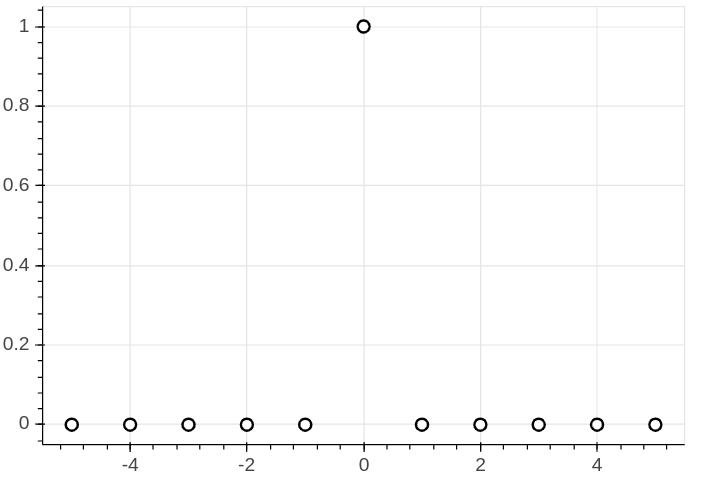
\includegraphics[width=4cm]{./Figuras/kronecker}\\%
            }\end{column}
            \begin{column}{0.65\textwidth}{\scriptsize
                \hspace{1.5cm}\color{olivegreen}$x[n]=\sum_{k=-\infty}^{\infty} x[k]\delta[k-n]$\color{black}\\
                \vspace{0.4cm}
                \hspace{1.5cm}$(x\! \ast\! \delta)[n] \!=\! \sum_{k=-\infty}^\infty x[k]\delta[n-k]=x[n]$
            }\end{column}
        \end{columns}
    \end{itemize}
\end{frame}
	
%%%%%%%%%%%%%%%%%%%%%%%%%%%%%%%%%%%%%%%%%%%%%%

\begin{frame}
\frametitle{Señales básicas: Escalón unitario}
  \begin{itemize}
    \begin{columns}[c]
        \begin{column}{7.0cm}
        
        \item \alert{Continuo:} $u(t)=\left \{ \begin{array}{l} 0 \:\: \: \:t<0\\1 \:\: \:\:  t \ge 0\end{array}\right .$

    \vspace{0.1cm}

        
        \small Relación con el impulso:

    \vspace{0.1cm}

    $\delta(t)=\frac{du(t)}{dt}$

    \vspace{0.1cm}

    $u(t)=\int _{-\infty} ^t \delta(\tau)d\tau$

    \vspace{0.1cm}

    Convolución: $(x \ast u)(t)=\int _{-\infty} ^t x(\tau)d\tau $
        
        \end{column}
    \hspace{-2.5cm}\begin{column}{5cm}
        \begin{figure}
    \centering
    \footnotesize
    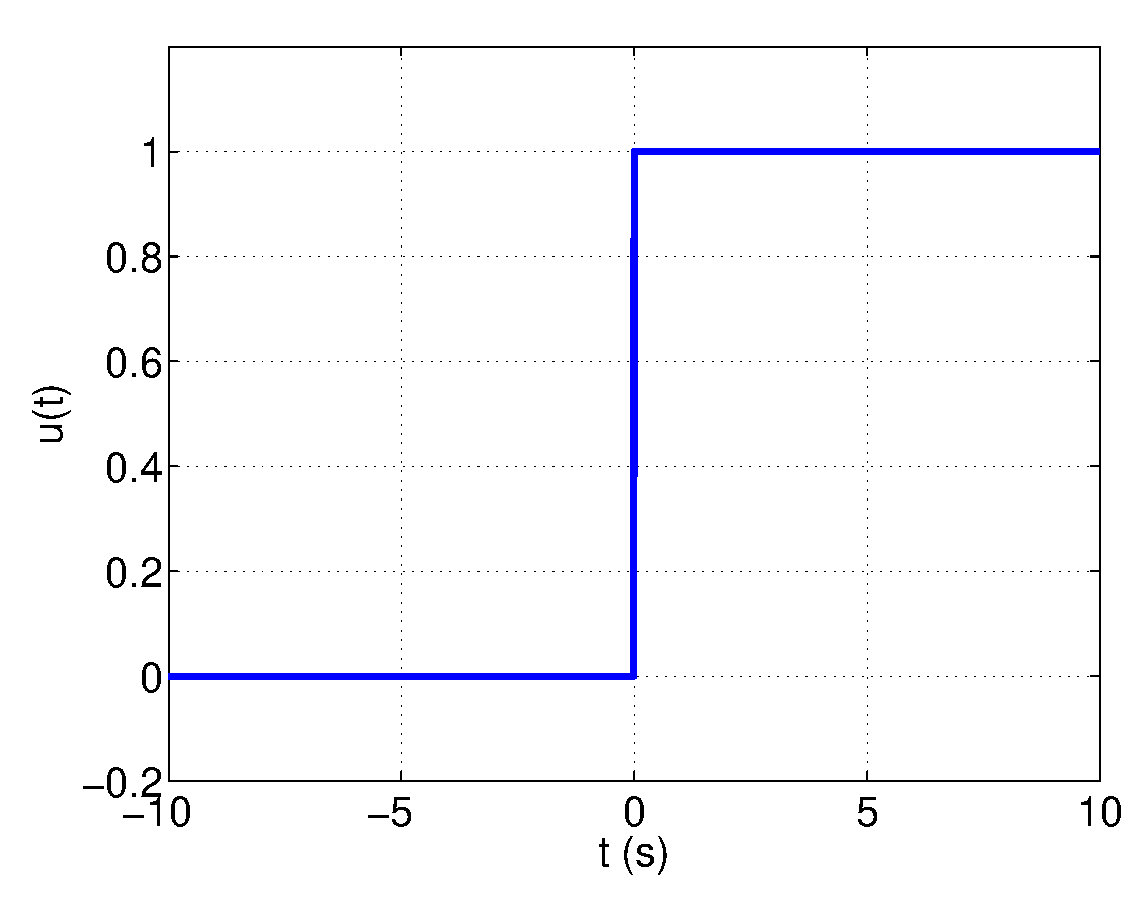
\includegraphics[width=4cm]{./Figuras/EscalonT.eps} 
    \end{figure}
        \end{column}
      \end{columns}
      
  \vspace{-0.2cm}

  \hspace{1cm}\begin{columns}[c]
      \begin{column}{6.0cm}
                      \item \alert{Discreto:}  $u[n]=\left \{ \begin{array}{l} 0\:\: \: \:n<0\\1 \:\: \:\:  n \ge 0\end{array}\right .$
      
              \vspace{0.2cm}
      
      \small Relación con el impulso:

  \vspace{0.2cm}

  $\delta[n]=u[n]-u[n-1]$

  \vspace{0.2cm}

  $u[n]=\sum _{k=-\infty} ^n \delta[k]$
      
      \vspace{0.2cm}

  Convolución: $(x\! \ast \! u)[n]\!=\!\sum _{k=-\infty} ^n x[k]$
      
      \end{column}
  \hspace{-1.5cm}\begin{column}{5cm}
      \begin{figure}
  \centering
  \footnotesize
  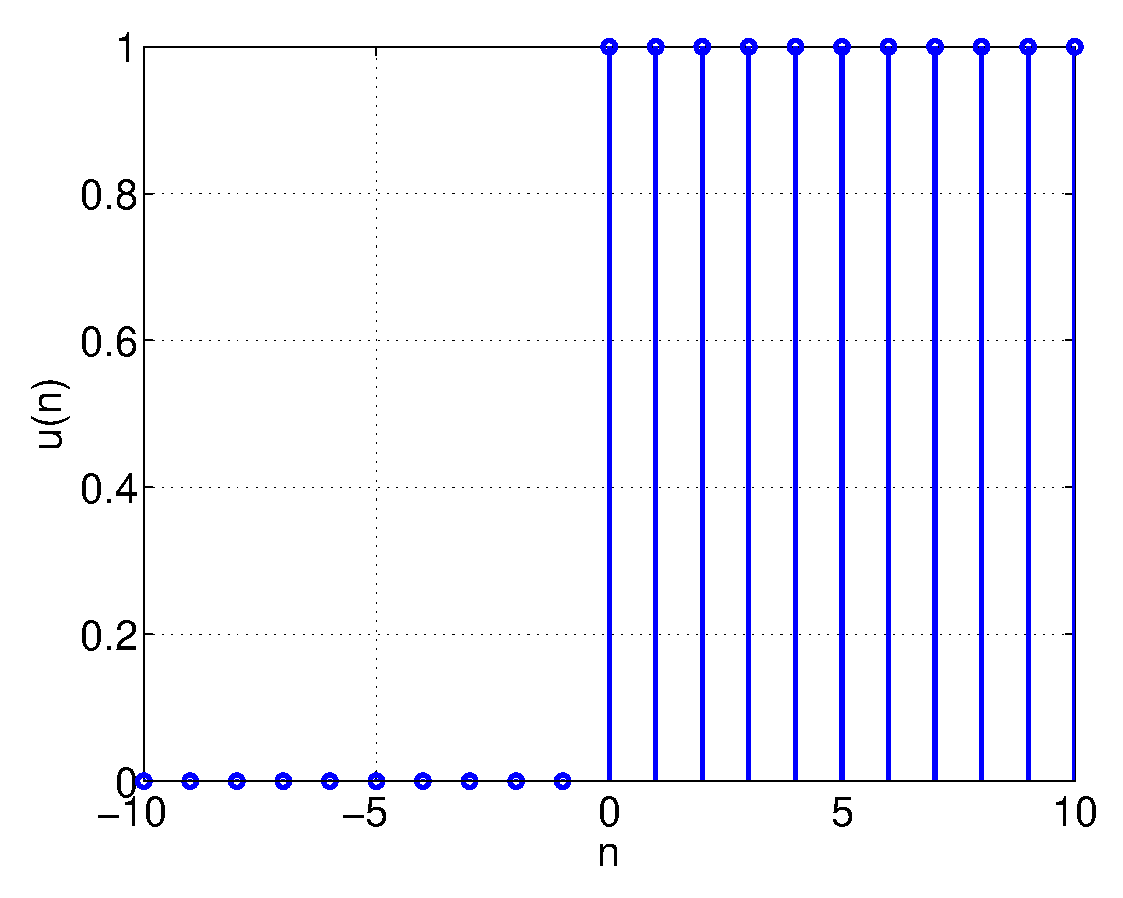
\includegraphics[width=4cm]{./Figuras/EscalonN.eps} 
  \end{figure}
      \end{column}
    \end{columns}
  \end{itemize}

  \small El producto de cualquier señal $x(\cdot)$ por $u(\cdot)$ produce una señal causal.
\end{frame}

%%%%%%%%%%%%%%%%%%%%%%%%%%%%%%%%%%%%%%%%%%%%%%%
	
	
\begin{frame}
\frametitle{Señales básicas: Rampa}

\begin{itemize}

\begin{columns}[c]
    \begin{column}{7.0cm}
        \item \alert{Continuo:} $r(t)=\left \{ \begin{array}{l} 0 \\ t \end{array}\begin{array}{l}t<0 \\ t \ge 0\end{array}\right .$

\vspace{0.1cm}

    
    \small Relación con el escalón:

\vspace{0.1cm}

$u(t)=\frac{dr(t)}{dt}$

\vspace{0.1cm}

$r(t)=\int _{-\infty} ^t u(\tau)d\tau$

\vspace{0.1cm}

    
    \end{column}
\hspace{-2.5cm}\begin{column}{5cm}
    \begin{figure}
\centering
\footnotesize
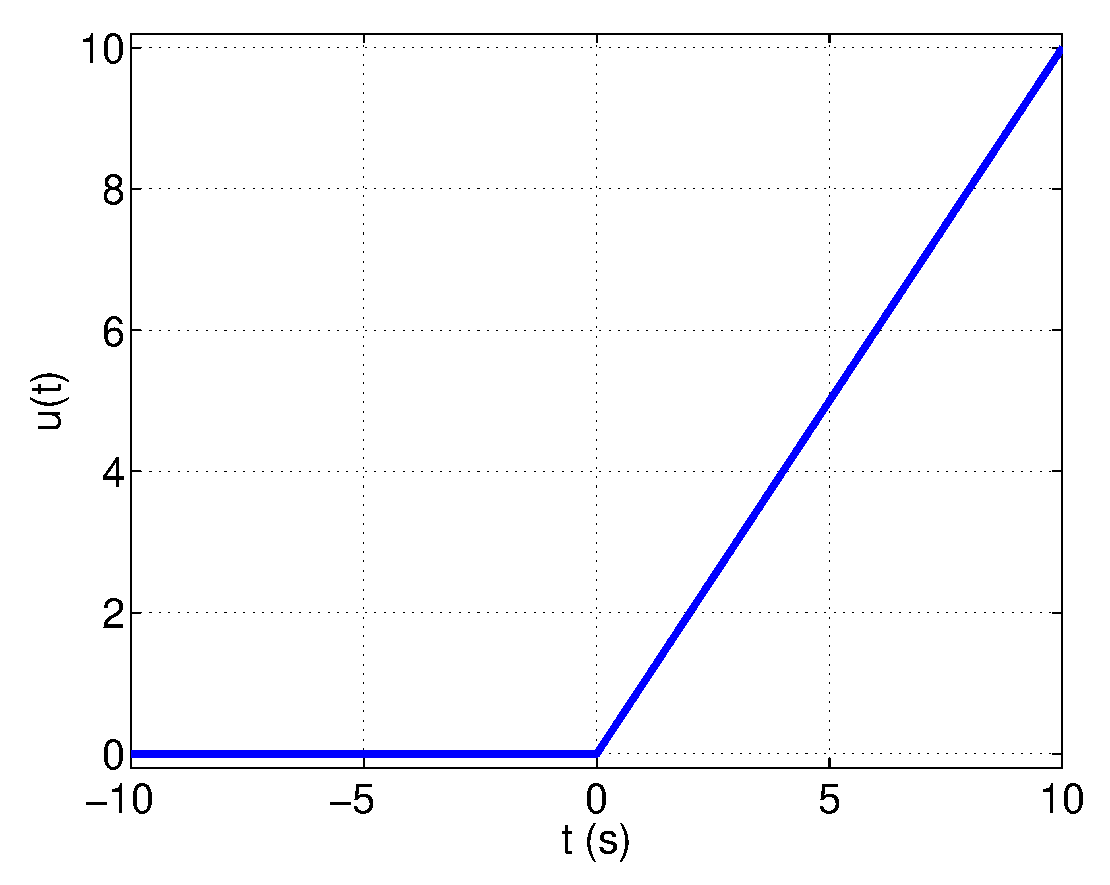
\includegraphics[width=4cm]{./Figuras/RampaT.eps} 
\end{figure}
    \end{column}
    \end{columns}
    
\vspace{-0.2cm}

\hspace{1cm}\begin{columns}[c]
    \begin{column}{6.0cm}
                    \item \alert{Discreto:}  $r[n]=\left \{ \begin{array}{l} 0 \\n+1\end{array}\begin{array}{l} n<0\\n \ge 0\end{array}\right .$
    
    
            \vspace{0.2cm}
    
    \small Relación con el escalón:

\vspace{0.2cm}

$u[n]=r[n]-r[n-1]$

\vspace{0.2cm}

$r[n]=\sum _{k=-\infty} ^n u[k]$
    
    \vspace{0.2cm}
    
    \end{column}
\hspace{-1.5cm}\begin{column}{5cm}
    \begin{figure}
\centering
\footnotesize
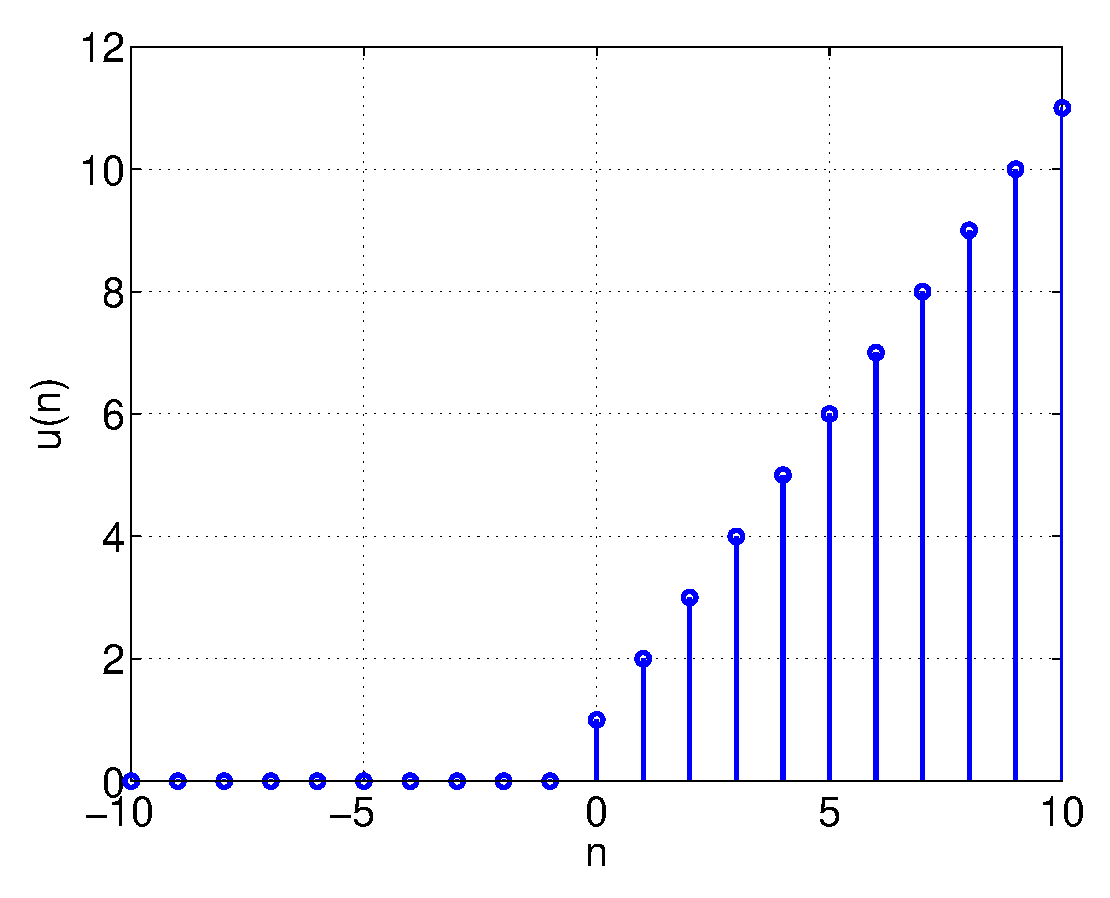
\includegraphics[width=4cm]{./Figuras/RampaN.eps} 
\end{figure}
    \end{column}
    \end{columns}


\end{itemize}


\end{frame}


%%%%%%%%%%%%%%%%%%%%%%%%%%%%%%%%%%%%%%%%%%%%%%

\begin{frame}\frametitle{Señales básicas: Pulsos}

    \begin{itemize}
        \begin{columns}[c]
            \begin{column}{5cm}
            \item \alert{Pulso rectangular}
                \vspace{0.3cm}
                $\Pi(t)=\left \{ \begin{array}{l} 1 \:\: \: \:|t| \le \frac{1}{2}\\0 \:\: \:\:  |t| > \frac{1}{2}\end{array}\right .$            
                \begin{figure}
                    \centering
                    \footnotesize
                    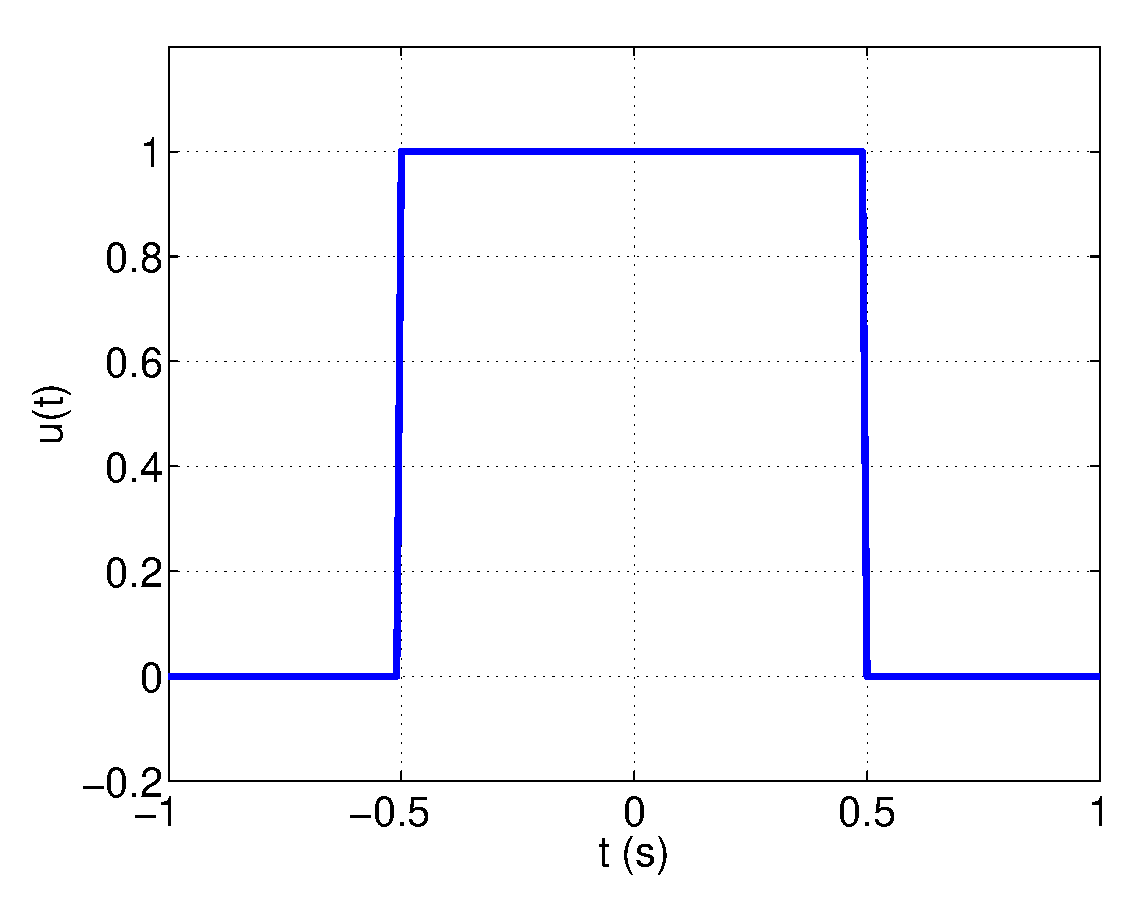
\includegraphics[width=5cm]{./Figuras/PulsoRect.eps} 
                \end{figure}
            \end{column}
            \begin{column}{5.cm}
                \item \alert{Pulso triangular}
                \vspace{0.3cm}
                $\Lambda(t)=\left \{\!\! \begin{array}{l} t+1 \:\: \: \:-1 \le t \le 0\\1-t \:\: \:\: \:\: \:\: \: 0 \le t \le 1\end{array}\right .$            
                \begin{figure}
                    \centering
                    \footnotesize
                    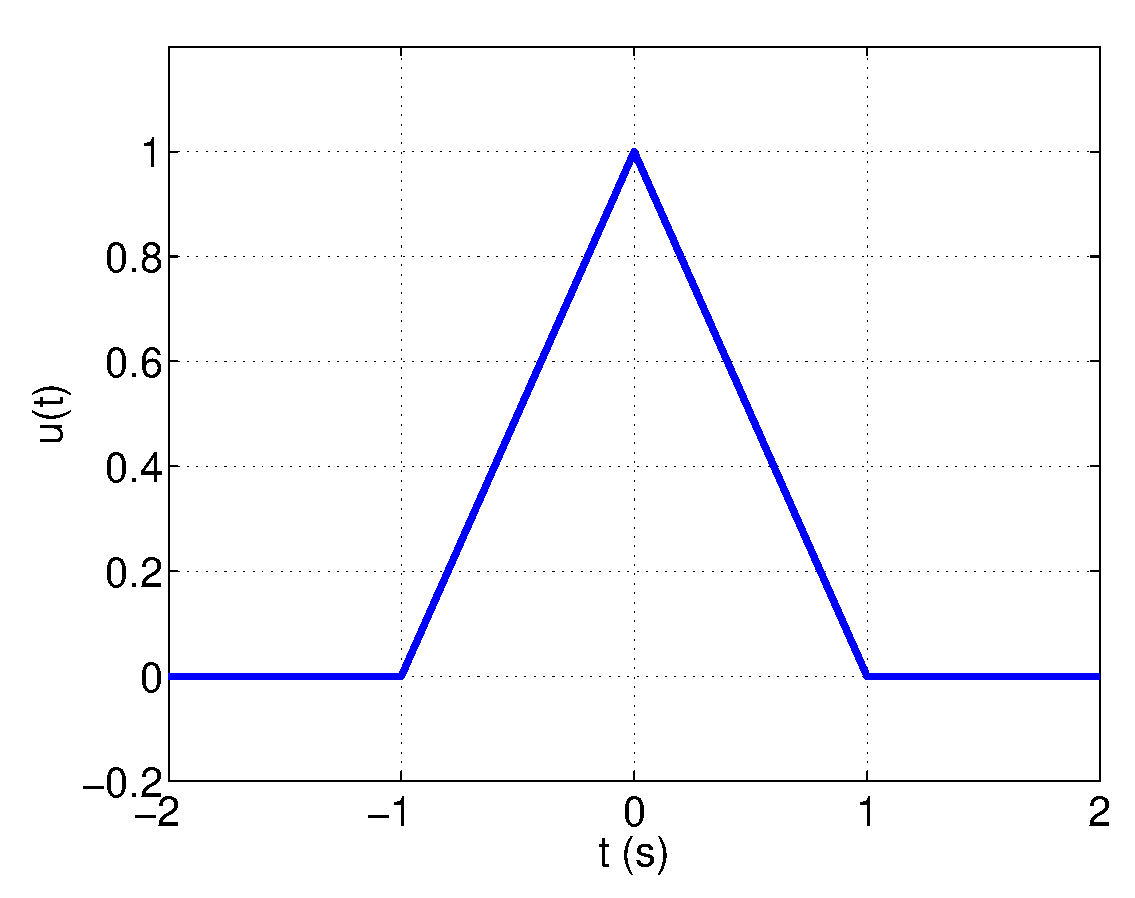
\includegraphics[width=5cm]{./Figuras/PulsoTri.eps} 
                \end{figure}
            \end{column}
        \end{columns}
    \end{itemize}
\end{frame}

%%%%%%%%%%%%%%%%%%%%%%%%%%%%%%%%%%%%%%%%%%%%%%%%%%%%%%
\begin{frame}
	\frametitle{Señales básicas: Exponencial Compleja}\centering
    \begin{itemize}
        \item \alert{Continua:} $x(t)=A\mathsf{e}^{\:j\omega t}$
		\begin{itemize}
            \item \color{blue}$x(t)=x(t+T)$\color{black}, con $T=\frac{1}{f}=\frac{2\pi}{\omega}$ \\
            \color{cyan}{\tiny $x(t+T)=A\mathsf{e}^{\:j\omega (t+\frac{2\pi}{\omega})}=A\mathsf{e}^{\:j(\omega t+2\pi)}=A\mathsf{e}^{\:j\omega t}\mathsf{e}^{\:j2\pi}=A\mathsf{e}^{\:j\omega t}$=x(t)}\color{black}
            \vspace{0.1cm}
            \item \color{blue}$\omega=2\pi f$ \color{black}es la frecuencia ($\omega$ rad/s, $f$ Hz)
            \vspace{0.1cm}
            \item \color{blue}$\omega_1\neq\omega_2 \Rightarrow x_1(t)\neq x_2(t)$\color{black}, para $0<\omega<\infty$
            \vspace{0.1cm}
        \end{itemize}
    \end{itemize}
    \begin{minipage}{0.25\textwidth}
        \centering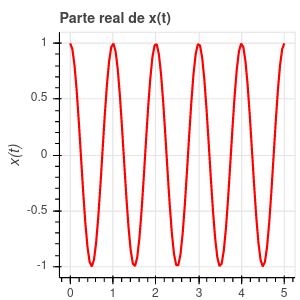
\includegraphics[width=\textwidth]{Figuras/exp_real.png}
    \end{minipage}
    \begin{minipage}{0.25\textwidth}
        \centering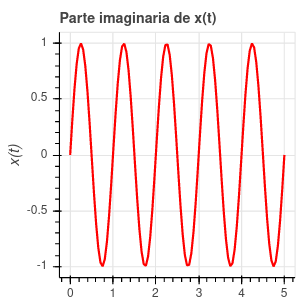
\includegraphics[width=\textwidth]{Figuras/exp_imag.png}
    \end{minipage}

    \begin{block}{{\scriptsize Fórmula de Euler}}\centering
        \scriptsize{$e^{j(\omega t+\phi)}=cos(\omega t+\phi)+j sin(\omega t+\phi)\Rightarrow \left\lbrace\begin{matrix}
            cos(\omega t+\phi)=\frac{e^{j(\omega t+\phi)}+e^{-j(\omega t+\phi)}}{2}\\
            sin(\omega t+\phi)=\frac{e^{j(\omega t+\phi)}-e^{-j(\omega t+\phi)}}{2j}\\
        \end{matrix}\right.$}
    \end{block}
\end{frame}


\begin{frame}
	\frametitle{Señales básicas: Exponencial Compleja}\centering

	\begin{itemize}
		\item \alert{Continua (Forma General):} $x(t)=C \mathsf{e}^{a t}$, con $C,a\in\mathbb{C}$
		\vspace{0.1cm}
		\begin{itemize}{\small
            \item $\left.\begin{matrix}C=|C|\mathsf{e}^{j\phi}\\a=r+j\omega\end{matrix}\right\rbrace \Rightarrow \color{blue}x(t)=|C| \mathsf{e}^{r t}\mathsf{e}^{\:j(\omega t+\phi)}\color{black}$
    %        \vspace{0.1cm}
            \item Sinusoidal multiplicada por exponencial
            \vspace{0.1cm}
            \item Decreciente ($r<0$), constante ($r=0$) o creciente ($r>0$)
            \vspace{0.1cm}
        }\end{itemize}
    \end{itemize}
    \begin{minipage}{0.25\textwidth}
        \centering\scriptsize{$r<0$}\\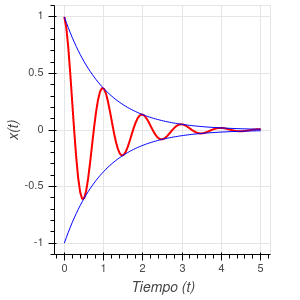
\includegraphics[width=\textwidth]{Figuras/exp_decreciente.png}
    \end{minipage}
    \begin{minipage}{0.25\textwidth}
        \centering\scriptsize{$r=0$}\\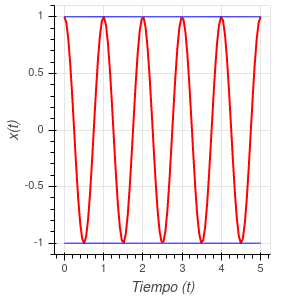
\includegraphics[width=\textwidth]{Figuras/exp_sin.png}
    \end{minipage}
    \begin{minipage}{0.25\textwidth}
        \centering\scriptsize{$r>0$}\\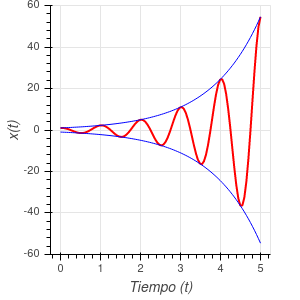
\includegraphics[width=\textwidth]{Figuras/exp_creciente.png}        
    \end{minipage}
    \begin{block}{{\scriptsize Fórmula de Euler}}\centering
        \scriptsize{$e^{j(\omega t+\phi)}=cos(\omega t+\phi)+j sin(\omega t+\phi)\Rightarrow \left\lbrace\begin{matrix}
            cos(\omega t+\phi)=\frac{e^{j(\omega t+\phi)}+e^{-j(\omega t+\phi)}}{2}\\
            sin(\omega t+\phi)=\frac{e^{j(\omega t+\phi)}-e^{-j(\omega t+\phi)}}{2j}\\
        \end{matrix}\right.$}
    \end{block}
\end{frame}


\begin{frame}
	\frametitle{Señales básicas: Exponencial Compleja}\centering
    \begin{itemize}
        \vspace{0.1cm}
		\item \alert{Discreta:} $x[n]=C \mathsf{e}^{j\omega n}$
		\begin{itemize}{\small
            \item \color{blue}$\omega=2\pi f$~\color{black} es la frecuencia en rad/muestra
            \vspace{0.1cm}
            \item \color{blue}$x[n]=x[n+N]$\color{black}, con $N=\frac{1}{f}=\frac{2\pi}{\omega}$ \color{red}sólo si \color{black}
            \vspace{0.1cm}
            \color{cyan}{\tiny $x[n+N]=C\mathsf{e}^{\:j\omega (n+N)}=C\mathsf{e}^{\:j(\omega n+\omega N)}=C\mathsf{e}^{\:j\omega n}\mathsf{e}^{\:j\omega N}=x[n]$\\
            \vspace{0.1cm}
            $\mathsf{e}^{\:j\omega N}=1\Rightarrow 2\pi f N=2\pi k \Rightarrow f=\frac{k}{N}$, para algún $N,k\in\mathbb{N}$\\
            Nota: $\frac{k}{N}$ es una fracción irreducible, en caso contrario $\frac{a}{b}=\frac{m\cdot k}{m\cdot N}=\frac{k}{N}$
            }\color{black}


            \vspace{0.1cm}
            \item \color{blue}$\omega_1\neq\omega_2 \Rightarrow x_1[n]\neq x_2[n]$\color{black}, \color{red}sólo para $0<\omega<2\pi\color{black}$\\
            \vspace{0.1cm}
            \color{cyan}{\scriptsize $\omega_k=\omega+2\pi k \Rightarrow$
            $C\mathsf{e}^{\:j(\omega + 2\pi k) n}=C\mathsf{e}^{\:j\omega n+j2\pi k n}=C\mathsf{e}^{\:j\omega n}\mathsf{e}^{\:j2\pi k n}=C\mathsf{e}^{\:j\omega n}$}\color{black}
            \vspace{0.1cm}
        }\end{itemize}
    \end{itemize}

    \begin{block}{{\scriptsize Fórmula de Euler}}
        \centering
        \scriptsize{$e^{j\omega n+\phi}=cos(\omega n+\phi)+j sin(\omega n+\phi)\Rightarrow \left\lbrace\begin{matrix}
            cos(\omega n+\phi)=\frac{e^{j(\omega n+\phi)}+e^{-j(\omega n+\phi)}}{2}\\
            sin(\omega n+\phi)=\frac{e^{j(\omega n+\phi)}-e^{-j(\omega n+\phi)}}{2j}\\
        \end{matrix}\right.$}
    \end{block}
\end{frame}


\begin{frame}
	\frametitle{Señales básicas: Exponencial Compleja}\centering
    \begin{itemize}{\scriptsize
        \vspace{0.1cm}
		\item \alert{Exponencial Discreta (sinusoidal):} $x[n]=C \alpha^n$, con $C,\alpha\in\mathbb{C}$
		\begin{itemize}{\scriptsize
            \item $\left.\begin{matrix}C=|C|e^{\phi}\\\alpha=|\alpha|e^{j\omega}\end{matrix}\right\rbrace \Rightarrow\color{blue}x(t)=|C||\alpha|^{n}e^{~j\omega n+\phi}\color{black}$
            \vspace{0.1cm}
            \item Decreciente ($0<\alpha<1$), constante ($\alpha=1$), o creciente ($\alpha>1$)
            \vspace{0.1cm}
        }\end{itemize}
    }\end{itemize}
    \begin{minipage}{0.25\textwidth}
        \centering\scriptsize{$0<|\alpha|<1$}\\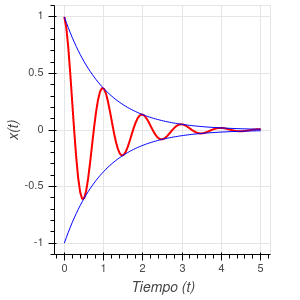
\includegraphics[width=\textwidth]{Figuras/exp_decreciente.png}
    \end{minipage}
    \begin{minipage}{0.25\textwidth}
        \centering\scriptsize{$|\alpha|=1$}\\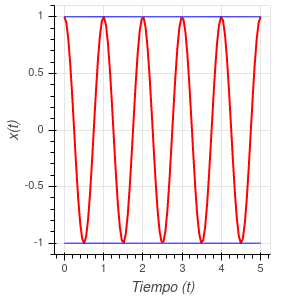
\includegraphics[width=\textwidth]{Figuras/exp_sin.png}
    \end{minipage}
    \begin{minipage}{0.25\textwidth}
        \centering\scriptsize{$|\alpha|>1$}\\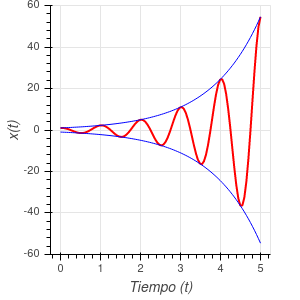
\includegraphics[width=\textwidth]{Figuras/exp_creciente.png}
    \end{minipage}

    \begin{block}{Fórmula de Euler}
        \centering
        \scriptsize{$e^{j\omega n+\phi}=cos(\omega n+\phi)+j sin(\omega n+\phi)\Rightarrow \begin{matrix}
            cos(\omega n+\phi)=\frac{e^{j\omega n+\phi}+e^{-j\omega n-\phi}}{2}\\
            sin(\omega n+\phi)=\frac{e^{j\omega n+\phi}-e^{-j\omega n-\phi}}{2}\\
        \end{matrix}$}
    \end{block}
\end{frame}



\begin{frame}
\frametitle{Señales básicas: muestreo, sinc, signo }

\vspace{-0.4cm}

\begin{itemize}



\begin{columns}[c]
    \begin{column}{4.5cm}
    
    \vspace{-0.8cm}
    
    \item \alert{Muestreo}

\vspace{0.3cm}

        $Sa(t)=\left \{ \begin{array}{l} \frac{sin(t)}{t} \:\: \: \:t \neq 0\\1 \:\: \:\: \:\: \:\: \:\: \:t=0\end{array}\right .$
        
            \item \alert{Sinc}

\vspace{0.3cm}

        $sinc(t)=\left \{\!\! \begin{array}{l} \frac{sin(\pi t)}{\pi t} \:\: \: \: t \ne 0 \\1 \:\: \:\:  \:\: \:\: \:\: \:\:  \: t=0\end{array}\right .$
    
    
    \vspace{0.7cm}
    
    
    \item \alert{Signo}

\vspace{0.3cm}

        $sgn(t)=\left \{\!\! \begin{array}{l} 1 \:\: \: \: \:\: \:\:t > 0 \\-1 \:\: \:\:   t<0 \\ 0  \:\: \:\:  \:\: \:\: t=0\end{array}\right .$


    
    \end{column}
\hspace{-0.5cm}	\begin{column}{4.5cm}
    
    \vspace{0.6cm}
            \begin{figure}
\centering
\footnotesize
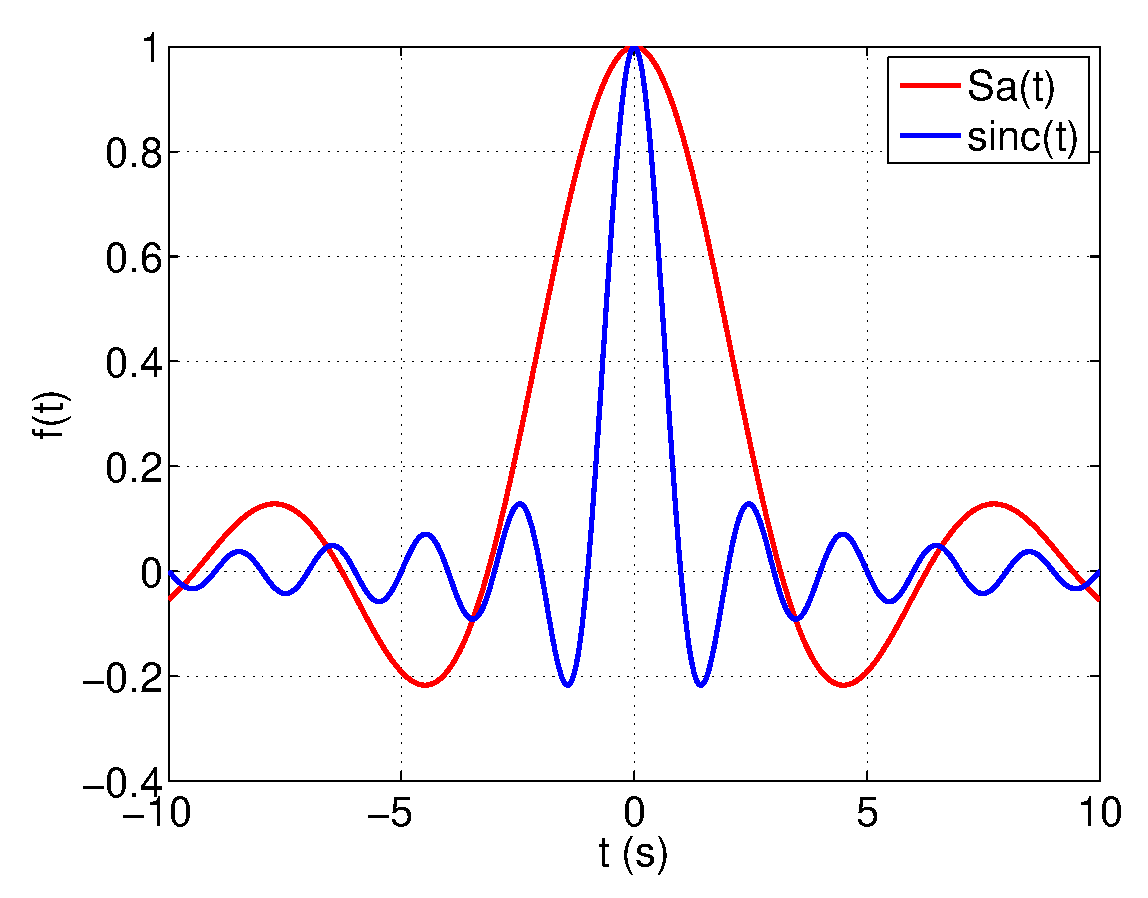
\includegraphics[width=4.5cm]{./Figuras/MuestreoSinc.eps} 
\end{figure}

            \begin{figure}
\centering
\footnotesize
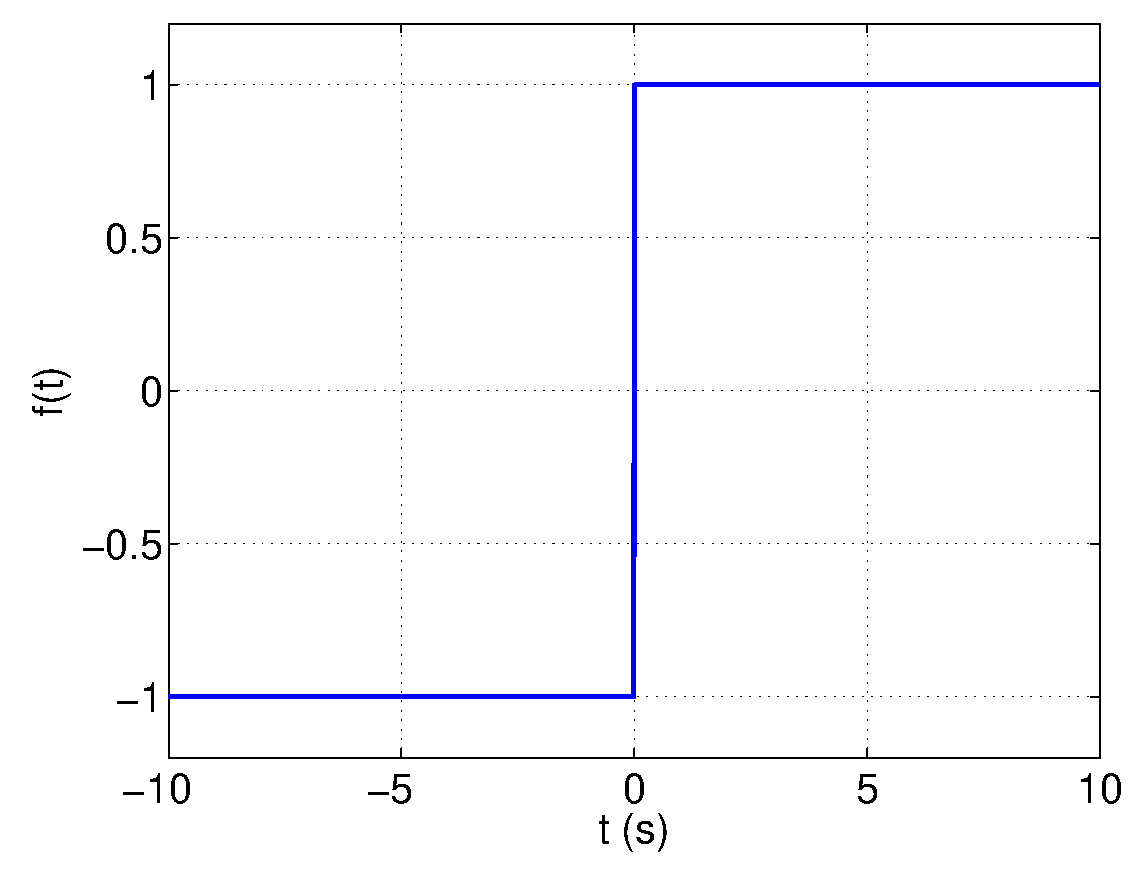
\includegraphics[width=4.5cm]{./Figuras/Signo.eps} 
\end{figure}

    
    \end{column}
    \end{columns}


\end{itemize}





\end{frame}

%%%%%%%%%%%%%%%%%%%%%%%%%%%%

\begin{frame}
\frametitle{Señales básicas: ondas  }

\begin{itemize}

\begin{columns}[c]
    \begin{column}{4.5cm}
    
    \item \alert{Onda cuadrada}

\vspace{0.3cm}

    
            
            \begin{figure}
\centering
\footnotesize
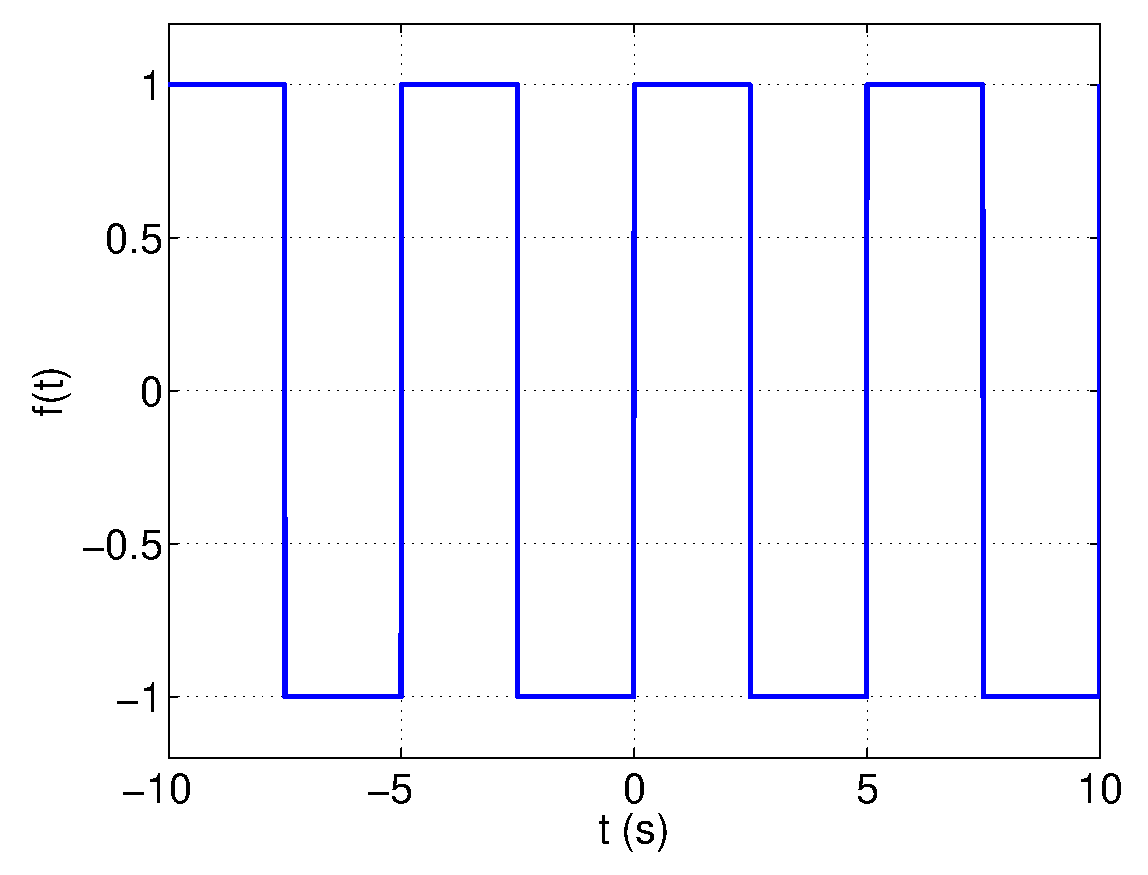
\includegraphics[width=4.5cm]{./Figuras/Square.eps} 

$T=5$
\end{figure}
    
    
    

    
    \end{column}
\hspace{-0.5cm}	\begin{column}{4.5cm}
    
        \item \alert{Onda triangular}

\vspace{0.3cm}




            \begin{figure}
\centering
\footnotesize
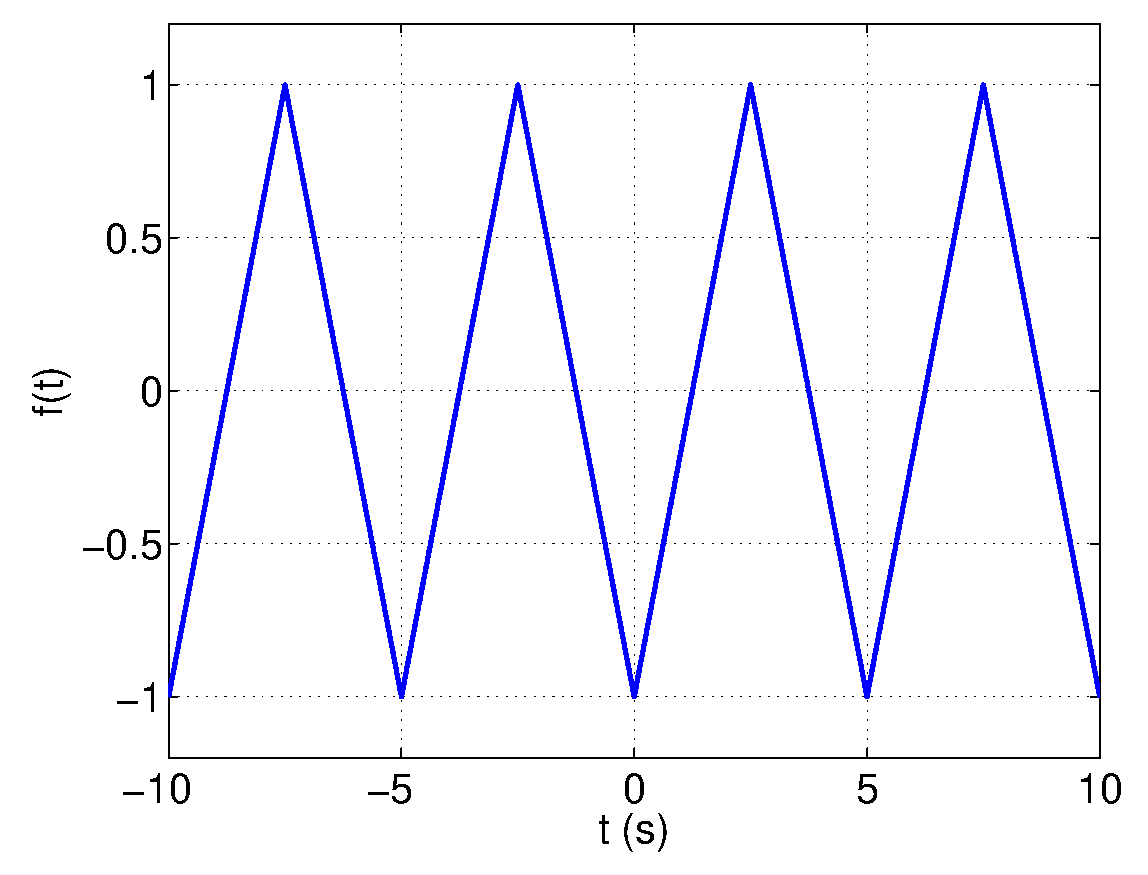
\includegraphics[width=4.5cm]{./Figuras/Triangular.eps} 

$T=5$
\end{figure}

    
    \end{column}
    \end{columns}


\end{itemize}

\end{frame}

\begin{frame}
\frametitle{Señales básicas: chirp  }

\begin{itemize}

\begin{columns}[c]

\hspace{-0.5cm}	\begin{column}{4.5cm}
    
        \item \alert{Chirp de variaci\'{o}n lineal}

\vspace{0.3cm}




\begin{figure}
    \centering
\footnotesize
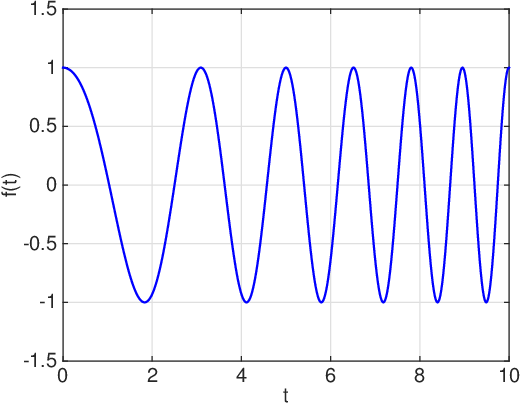
\includegraphics[width=4.5cm]{./Figuras/chirp} 

$f_{t=0}=0.2$ y $f_{t=10}=1$ 
\end{figure}

    
    \end{column}
    \end{columns}


\end{itemize}

\end{frame}


\begin{frame}\frametitle{Conceptos importantes}
  \begin{itemize}
    \item \alert{Definición de señal y sistema.}
    \item \alert{Clasificación de señales según sus características.}
    \begin{itemize}
      \item Analógica - Digital
      \item Periódica - Aperiódica
      \item Energía finita - Potencia finita - Señales no físicas
    \end{itemize}
    \item \alert{Señales básicas.}
    \begin{itemize}
      \item Impulso, Pulso (rectangular, triangular).
      \item Senoidales, Exponencial compleja.
      \item Exponencial real.
      \item Señales periódicas.
      \item Muestreo, sinc.
    \end{itemize}
  \end{itemize}
\end{frame}
%%%%%%%%%%%%%%%%%%%%%%%%%%%%%%%%%%%%%%%%%%%%%%

\begin{frame}
    \frametitle{Operaciones sobre la variable independiente I}
    \begin{itemize}
        \item Transformación $f(t)$ en la variable independiente:\\
        \vspace{0.1cm}
        \begin{center}
            \color{blue}$x(t)\Rightarrow y(t) = x(f(t))$, \hspace{0.1cm} $x[n] \Rightarrow y[n]=x[f(n)]$\color{black}
        \end{center}
        \vspace{0.1cm}
        \item Aunque no alteran los valores de la señal, pueden... 
        \vspace{0.2cm}
        \begin{itemize}
            \item alterar la forma
            \item provocar la pérdida de muestras (caso discreto).
        \end{itemize}
        \vspace{0.2cm}
        \item Suponemos\footnote{Veremos otras transformaciones en el Tema 5} \color{blue}$f(t)=\alpha t+\beta$\color{black}
        \vspace{0.4cm}

        \begingroup
            \small
            \begin{tabular}{r|ll}
                & continuo & discreto\\\hline
                \color{red}Desplazamiento:\color{black} & $y(t)=x(t-t_0)$ & $y[n]=x[n-n_0]$ \\
                \color{red}Inversión:\color{black} & $y(t)=x(-t)$ & $y[n]=x[-n]$ \\
                \color{red}Compresión/Expansión:\color{black} & $y(t)=x(\alpha t)$ & $y[n]=x[Kn]$ \\
            \end{tabular}
        \endgroup
    \end{itemize}
\end{frame}

%%%%%%%%%%%%%%%%%%%%%%%%%%%%%%%%%%%%%%%%%%%%%%

\begin{frame}
  \frametitle{Operaciones sobre la variable independiente II}
  \vspace{-0.1cm}
  \begin{itemize}
    \item <1-> \alert{Desplazamiento temporal:}
    \begin{itemize}
      \vspace{0.1cm}
      \item Continuo: $x(t) \: \rightarrow y(t)=x(t-t_0)$
      \vspace{0.1cm}
      \item Discreto: $x[n] \: \rightarrow y[n]=x[n-N_0]$
    \end{itemize}
    \vspace{0.2cm}
    \item <1-> \alert{Inversión:}
    \begin{itemize}
      \vspace{0.1cm}
      \item Continuo: $x(t) \: \rightarrow y(t)=x(-t)$
      \vspace{0.1cm}
      \item Discreto: $x[n] \: \rightarrow y[n]=x[-n]$
    \end{itemize}
  \end{itemize}
  \vspace{-0.3cm}
  \begin{figure}
    \centering
    \footnotesize
    \begin{tabular}{@{\extracolsep{-8pt}}cc}
      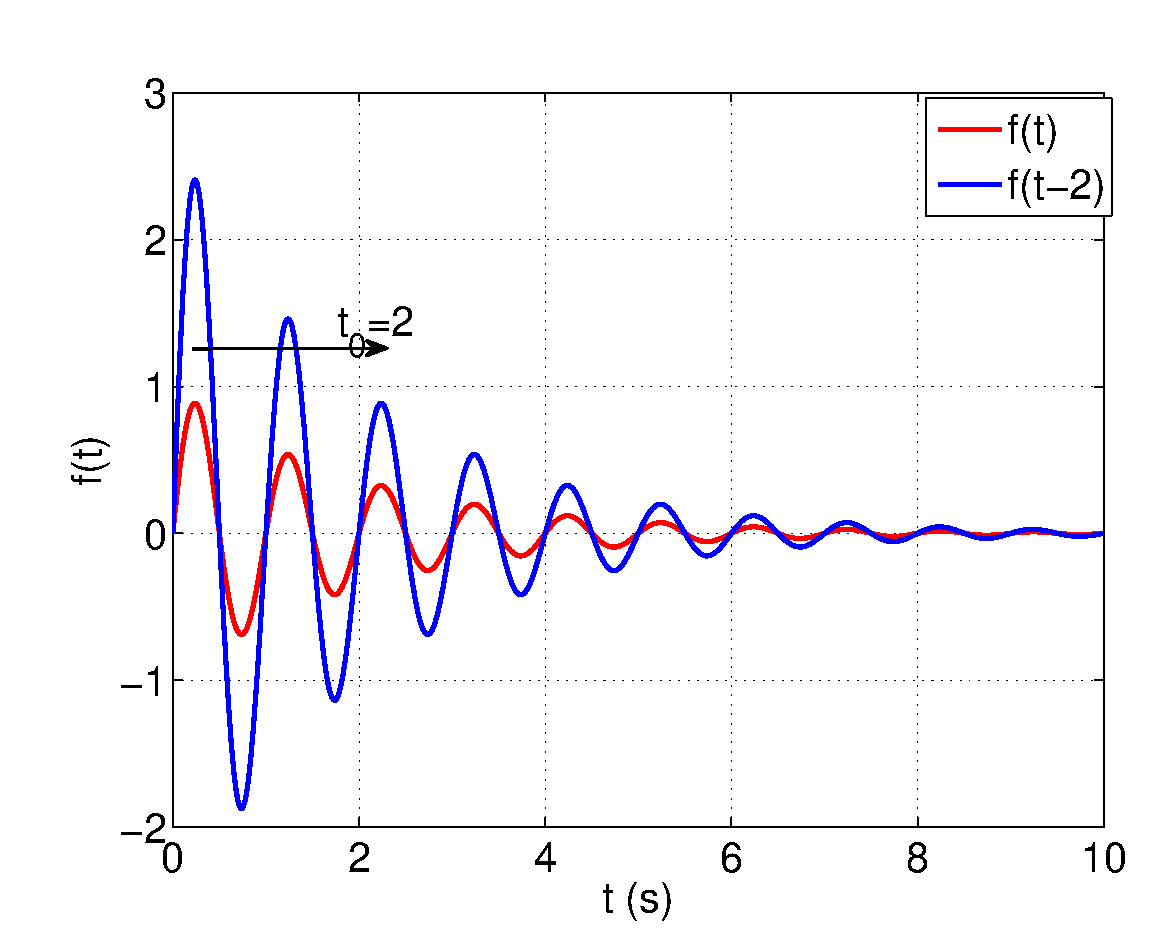
\includegraphics[width=4.5cm]{./Figuras/Figures/DesplazamientoT.eps}&
      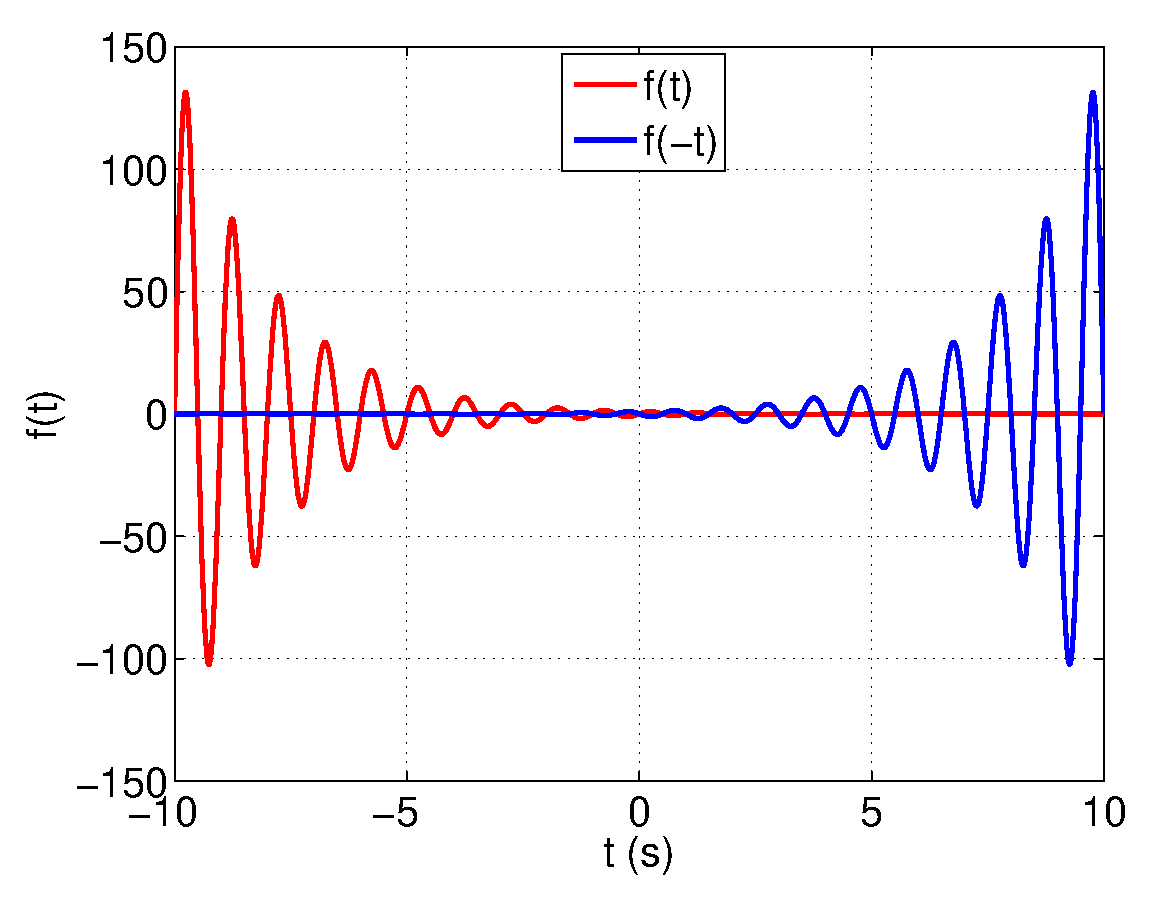
\includegraphics[width=4.5cm]{./Figuras/Figures/Inversion.eps} \\
      Desplazamiento  & Inversión
    \end{tabular}
  \end{figure}
\end{frame}

%%%%%%%%%%%%%%%%%%%%%%%%%%%%%%%%%%%%%%%%%%%%%%

\begin{frame}
  \frametitle{Operaciones sobre la variable independiente III}
  \vspace{-0.1cm}
  \begin{itemize}
    \item <1-> \alert{Compresión/expansión temporal}:
    \begin{itemize}
      \vspace{0.1cm}
      \item Continuo (escalado): \color{blue}$x(t) \: \rightarrow y(t)=x(\alpha \cdot t), \alpha>0$\color{black}
      \begin{itemize}
        \item Compresión ($\alpha > 1$), Expansión ($\alpha < 1$) 
      \end{itemize}
      \vspace{0.1cm}
      \item Discreto:
      \vspace{0.1cm}
      \begin{itemize}
        \item Diezmado:  \color{blue}$x[n] \: \rightarrow y[n]=x[N\cdot n], N \in \mathbb{Z}^+$\color{black}
        \vspace{0.1cm}
        \item Interpolación: \color{blue}$x[n] \: \rightarrow y[n]=x[\frac{n}{N}], N \in \mathbb{Z}^+$\color{black} \\
            \color{cyan}{\scriptsize no existe muestra para $\frac{n}{N}$ no entero, necesario generar}\color{black}
      \end{itemize}
    \end{itemize}
  \end{itemize}
  \vspace{-0.3cm}
  \begin{figure}
    \centering
    \footnotesize
    \begin{tabular}{@{\extracolsep{-8pt}}cc}
      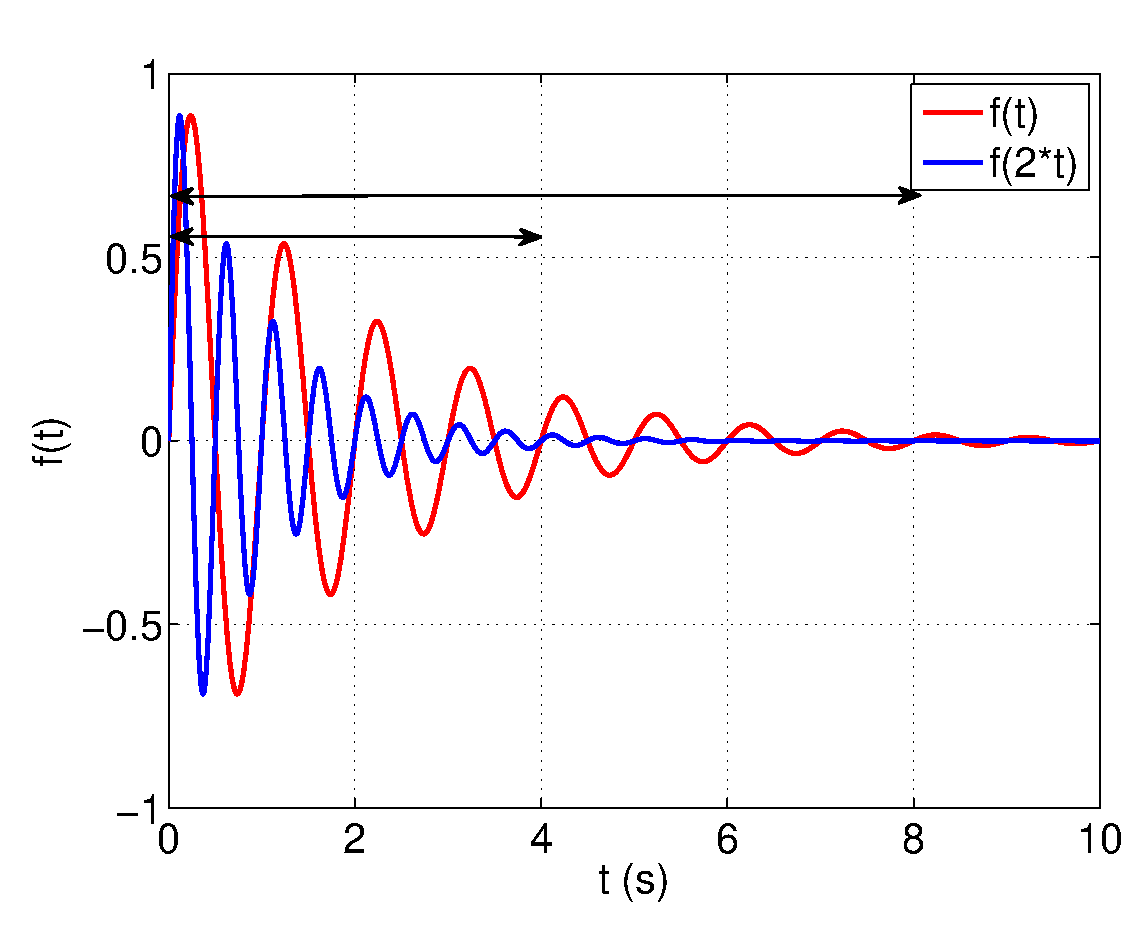
\includegraphics[width=4.5cm]{./Figuras/Figures/EscaladoT.eps}&
      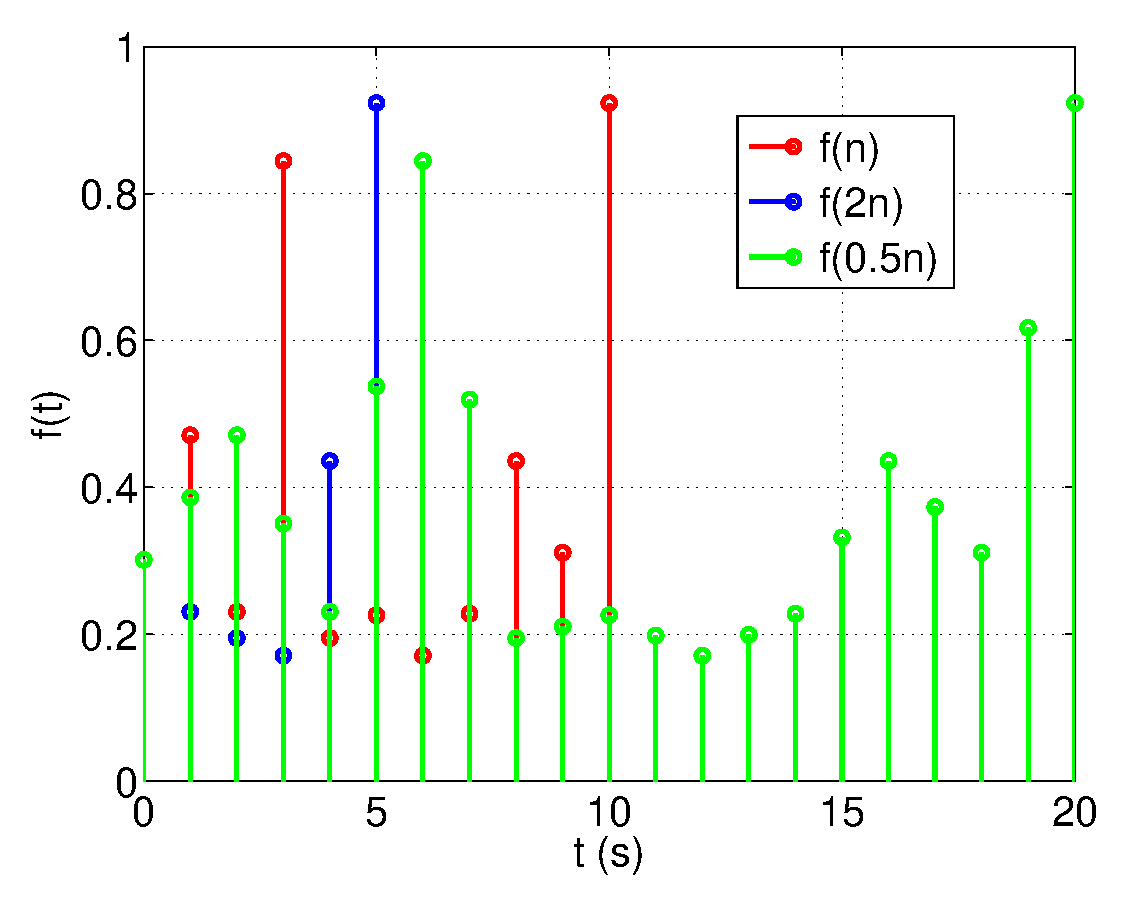
\includegraphics[width=4.4cm]{./Figuras/Figures/EscaladoD.eps} \\
      Escalado & Diezmado \& Interpolación
    \end{tabular}
  \end{figure}
\end{frame}

% %%%%%%%%%%%%%%%%%%%%%%%%%%%%%%%%%%%%%%%%%%%%%%%%%%%

\begin{frame}
  \frametitle{Operaciones básicas sobre la señal}
  \begin{itemize}
    \item \color{red}Generales\color{black}:
    \begin{itemize}
      \vspace{0.1cm}
      \item  {Suma/Resta/Multiplicación/División}:\\
      \vspace{0.1cm}
      \color{blue}$x_1(\cdot) \pm x_2(\cdot)$,   $\:\:x_1(\cdot) \cdot x_2(\cdot)$,  $\:\:x_1(\cdot) \div x_2(\cdot)$\color{black}
    \end{itemize}
    \vspace{0.1cm}
    \item{\color{red}Continuas\color{black}}:
    \begin{itemize}
      \vspace{0.1cm}
      \item Derivación: \color{blue}$y(t)=\frac{dx(t)}{dt}$\color{black}
      \vspace{0.2cm}
      \item Integración: \color{blue}$y(t)=\int_{\tau=-\infty}^t x(\tau) d\tau$\color{black}
      \vspace{0.1cm}
    \end{itemize}
    \item{\color{red}Discretas\color{black}}:
    \begin{itemize}
      \vspace{0.1cm}
      \item Diferencia: \color{blue}$y[n]=x[n]-x[n-1]$\color{black}
      \vspace{0.2cm}
      \item Acumulación: \color{blue}$x[n]=\sum_{k=-\infty}^n x[k]$\color{blue}
      \vspace{0.1cm}
    \end{itemize}
  \end{itemize}
\end{frame}

% %%%%%%%%%%%%%%%%%%%%%%%%%%%%%%%%%%%%%%%%%%%%%%%%%%%

\begin{frame}
  \frametitle{Convolución}
  \begin{itemize}
    \item Convolución de dos señales:
    \vspace{0.1cm}
    \begin{itemize}
      \item \alert{Señales continuas}: \small \color{blue}$(x \ast y)(t)=\int_{-\infty}^\infty x(\tau)y(t-\tau)d\tau$\color{black}
      \vspace{0.1cm}
      \item \alert{Señales discretas}: \small \color{blue}$(x \ast y)[n]=\sum_{k=-\infty}^\infty x[k]y[n-k]$\color{black}
      \begin{itemize}
        \vspace{0.2cm}
        \item Invertir:\quad\quad \color{cyan}$y(-\tau), y[-k].$\color{black}
        \item Desplazar:~~ \color{cyan}$y(t-\tau), y[n-k].$\color{black}
        \item Multiplicar:~~ \color{cyan}$x(\tau)y(t-\tau), x[k]y(n-k).$\color{black}
        \item Sumar:\quad\quad \color{cyan}$\int, \sum.$\color{black}
      \end{itemize}
    \end{itemize}
    \vspace{0.2cm}
    \item Propiedades:
    \begin{itemize}
      \small
      \item Conmutativa:  $(x \ast y)(\cdot)=(y\ast x)(\cdot)$
      \item Asociativa: $(x \ast y \ast z)(\cdot)=[(x \ast y) \ast z](\cdot)=[x \ast( y \ast z)](\cdot)$
      \item Distributiva: $((x+y) \ast z)(\cdot)=(x \ast z)(\cdot)+(y \ast z)(\cdot)$
      \item Respecto al impulso y al escalón  (más adelante)
    \end{itemize}
  \end{itemize}
\end{frame}


\begin{frame}\frametitle{Fourier (Cuadro resumen)}
  
  \centering
  \begin{tabular}{>{\columncolor{lightgray}}ccc}
    \rowcolor{lightgray}
    & \color{blue}\small \alert{Continua}  & \color{blue}\small  \alert{Discreta}\\
    \rotatebox{90}{\color{red}\small Periódica\color{black}}    & \parbox{4cm}{\centering\tiny Series de Fourier Continuas (CFS)\\\color{blue}$c[k]=\frac{1}{T}\int_{-T/2}^{T/2}{x(t)e^{-j k\omega_0 t}dt}$\color{black}\\\color{blue}$x(t)=\sum_{k=-\infty}^{\infty}{c[k]e^{j k\omega_0 t}}$\color{black}} & \parbox{3.5cm}{\centering\tiny Series de Fourier Discretas (DFS)\\\color{blue}$c[k]=\frac{1}{N}\sum_{n=0}^{N-1}{x[n]e^{-j\frac{2\pi}{N} k n}}$\color{black}\\\color{blue}$x[n]=\sum_{k=0}^{N-1}{c[k]e^{j\frac{2\pi}{N} k n}}$\color{black}} \\\\
    \rotatebox{90}{\color{red}\small Aperiódica\color{black}}   & \parbox{4cm}{\centering\tiny Trasnformada de Fourier\\de Tiempo Continuo (CTFT)\\\color{blue}$X(j\omega)= \int_{-\infty}^{\infty} x(t) e^{j\omega t} dt $\color{black}\\\color{blue}$x(t)=\frac{1}{2\pi}\int_{-\infty}^{\infty}{X(j\omega)e^{j\omega t}d\omega}$\color{black}} & \parbox{4cm}{\centering\tiny Trasnformada de Fourier\\de Tiempo Discreto (DTFT)\\\color{blue}$X(e^{j\omega})=\sum_{k=-\infty}^{\infty}{x[n]e^{-j\omega n}}$\color{black}\\\vspace{0.1cm}\color{blue}$x[n]=\frac{1}{2\pi}\int_{0}^{2\pi}{X(e^{j\omega})e^{j\omega n}d\omega}$\color{black}} \\
  \end{tabular}
  \begin{flushleft}
    \small
    \begin{itemize}
      \item Transformada de Fourier Discreta (DFT):
      \begin{itemize}
        \item \color{blue}$X[k]=\sum_{n=0}^{N-1}{x[n]e^{-j\frac{2\pi}{N} k n}}$\color{black}\\\vspace{0.1cm}
        \item \color{blue}$x[n]=\frac{1}{N}\sum_{k=0}^{N-1}{X[k]e^{j\frac{2\pi}{N} k n}}$\color{black}
      \end{itemize}
  \end{itemize}
  \end{flushleft}
\end{frame}


\begin{frame}
  \frametitle{Desarrollo en serie de Fourier: Se\~{n}ales peri\'{o}dicas}
  \vspace{-0.1cm}
  \small
  \begin{itemize}
    \item \color{red}Señales continuas\color{black}:  \color{blue}$x(t)=x(t+T)$, $\omega_0=2\pi/T$\color{black}
    \begin{itemize}
      \footnotesize
      \item Desarrollo en exponenciales complejas:\\
      \vspace{0.1cm}
      $\color{blue}\bullet\color{black}$ S\'{i}ntesis: \color{blue}$x(t)=\sum_{k=-\infty}^\infty c_k e^{jk\omega_0t}$\color{black}\\
      $\color{blue}\bullet\color{black}$  Análisis:  \color{blue}$c_k=\frac{1}{T } \int_{T} x(t) e^{-jk\omega_0t} dt $\color{black}
      \vspace{0.1cm}
      \visible<2->{
      \item Desarrollo en senos y cosenos ($x(t)$ es real):\\
      \vspace{0.1cm}
      $\color{blue}\bullet\color{black}$ S\'{i}ntesis:  $x(t)=\frac{a_0}{2}+\sum_{k=1}^{\infty} \left (a_k cos(k\omega_0t) + b_k sin(k\omega_0t)\right )$\\
      $\color{blue}\bullet\color{black}$  Análisis:  $ a_k=\frac{2}{T}\!\int_T x(t) cos(k\omega_0t)dt, \: \: b_k=\frac{2}{T}\!\int_T x(t) sin(k\omega_0t)dt$}
      \vspace{0.1cm}
    \end{itemize}
    \item \alert{Señales discretas}:  \color{blue}$x[n]=x[n+N]$, $\omega_0=2\pi/N$\color{black}
    \begin{itemize}
      \footnotesize
      \visible<3->{
      \item Desarrollo en exponenciales complejas:\\
      \vspace{0.1cm}
      $\color{blue}\bullet\color{black}$ S\'{i}ntesis: \color{blue}$x[n]=\sum_{k=0}^{N-1} c_k e^{j\omega_0kn}$\color{black}\\
      $\color{blue}\bullet\color{black}$ Análisis:  \color{blue}$c_k=\frac{1}{N } \sum_{n=0}^{N-1} x[n] e^{-j\omega_0kn} $\color{black}, $c_k=c_{k+N}$}
      \vspace{0.1cm}
      \visible<4->{
      \item Desarrollo en senos y cosenos ($x[t]$ es real):\\
      \vspace{0.1cm}
      $\color{blue}\bullet\color{black}$ $L=\frac{N}{2}\qquad \quad$ o $\quad L=\frac{N-1}{2}$\\
      $\color{blue}\bullet\color{black}$ $LIM=L-1\;$ o $\quad K=L$\\
      $\color{blue}\bullet\color{black}$ S\'{i}ntesis:  $x(n)=\frac{a_0}{2}+\sum_{k=1}^{LIM} \left (a_k cos(k\omega_0kt) + b_k sin(\omega_0kt)\right )$\\
      $\color{blue}\bullet\color{black}$  Análisis:  ${ a_k=\frac{2}{N}\sum_{n=0}^{N-1} x(n) cos(\omega kn), \: \: b_k=\frac{2}{N}\!\sum_{n=0}^{N-1} x(n) sin(\omega kn)}$}
      \vspace{0.1cm}
    \end{itemize}
  \end{itemize}
\end{frame}

%%%%%%%%%%%%%%%%%%%%%%
\begin{frame}
  \frametitle{Transformadas}
  % \vspace{-0.2cm}
  \begin{itemize}
    \item \alert{Serie vs. Transformada}
    \begin{itemize}
      \item \alert{Si una señal es periódica}
      \begin{itemize}
        \item Representación mediante exp. armónicas: $\phi_k(t)=\mathrm{e}^{\:jk \omega_0 t}$. 
        \item Combinación lineal: $x(t)=\sum_{k=-\infty}^{\infty}a_k\phi_k(t)$.
      \end{itemize}
      \item \alert{Si una señal es aperiódica:}
      \begin{itemize}
        \footnotesize
        \item El sumatorio pasa a ser una integral: $\int_{\omega=-\infty}^{\infty}X(\omega)\phi(\omega)d\omega$.
        \vspace{0.1cm}
      \end{itemize}
    \end{itemize}
    \item \alert{Transformada de Fourier, Laplace y Z:}
    \begin{itemize}
      \footnotesize
      \vspace{0.1cm}
      \item \alert{Se\~{n}ales continuas $x(t)$}:
      \begin{itemize}
        \footnotesize
        \item Transformada de Fourier: \color{blue}$X(j\omega_c)= \int_{-\infty}^{\infty} x(t) e^{-j\omega_c t} dt $\color{black}
        \item Transformada de Laplace: \color{blue}$X(s)=\int_{0}^{\infty} x(t) e^{-st} dt$\color{black}
        \item $s=\sigma \pm j\omega$
      \end{itemize}
      \visible<2->{
      \item \alert{Se\~{n}ales discretas $x[n]$}:
      \footnotesize
      \begin{itemize}
        \footnotesize
        \item T. de Fourier en tiempo discreto: \color{blue}$X(e^{j\omega_d})= \sum_{n=-\infty}^{\infty} x[n] e^{-j\omega_dn} $\color{black}
        \item Transformada Z: \color{blue}$X(z)=\sum_{n=0}^{\infty} x[n] z^{-n}$\color{black}
        \item  $X(e^{j\omega_d})$ es periodica (se repite en frecuencias cada $2\pi$)
        \item $z=e^{j\omega_d}$
        \item Si muestreamos periodicamente: $t=nT$, $z=e^{sT}$
      \end{itemize}
    }\end{itemize}
  \end{itemize}
\end{frame}

%%%%%%%%%%%%%%%%%%%%%%
\begin{frame}
  \frametitle{Transformadas}
  \vspace{-0.3cm}
  \begin{itemize}
    \item \alert{Comparación entre transformadas y sus usos:}
    \begin{itemize}
      \footnotesize
      \visible<3->{
      \item Transformada de Laplace y Z permiten:
      \begin{itemize}
        \scriptsize
        \item Resolver ecuaciones diferenciales (en diferencias)
        \item Obtener la funci\'{o}n de transferencia de sistemas LTI y su respuesta temporal a trav\'{e}s de la transformada inversa del producto de la funci\'{o}n de transferencia y la transformada de la entrada.
        \item Ver la respuesta a las condiciones iniciales.
      \end{itemize}
      }
      \visible<4->{
      \item Fourier (CTFT y DTFT) permite:
      \footnotesize
      \begin{itemize}
        \scriptsize
        \item Estudiar el comportamiento en frecuencia de las se\~{n}ales y de los sistemas.
        \item  Obtener la repuesta permanente de sistemas LTI estables como la transformada inversa del producto de la transformada de Fourier del sistema  con la transformada de la entrada.
      \end{itemize}
      }
    \end{itemize}
  \end{itemize}
\end{frame}


\begin{frame}\frametitle{Conceptos importantes}
  \begin{itemize}
    \item \alert{Operaciones sobre la variable independiente}
    \begin{itemize}
      \item Desplazamiento
      \item Inversión
      \item Compresión/Expansión
    \end{itemize}
    \item \alert{Operaciones básicas.}
    \begin{itemize}
      \item Generales (suma, resta, multiplicación, división)
      \item Derivación / Diferencia
      \item Integración / Acumulación
    \end{itemize}
    \item \alert{Convolución}
    \item \alert{Fourier}
  \end{itemize}
\end{frame}
\begin{frame}
	\frametitle{Señales básicas: Exponencial Compleja}\centering
    \begin{itemize}
        \item \alert{Continua:} $x(t)=A\mathsf{e}^{\:j\omega t}$
		\begin{itemize}
            \item \color{blue}$x(t)=x(t+T)$\color{black}, con $T=\frac{1}{f}=\frac{2\pi}{\omega}$ \\
            \color{cyan}{\tiny $x(t+T)=A\mathsf{e}^{\:j\omega (t+\frac{2\pi}{\omega})}=A\mathsf{e}^{\:j(\omega t+2\pi)}=A\mathsf{e}^{\:j\omega t}\mathsf{e}^{\:j2\pi}=A\mathsf{e}^{\:j\omega t}$=x(t)}\color{black}
            \vspace{0.1cm}
            \item \color{blue}$\omega=2\pi f$ \color{black}es la frecuencia ($\omega$ rad/s, $f$ Hz)
            \vspace{0.1cm}
            \item \color{blue}$\omega_1\neq\omega_2 \Rightarrow x_1(t)\neq x_2(t)$\color{black}, para $0<\omega<\infty$
            \vspace{0.1cm}
        \end{itemize}
    \end{itemize}
    \begin{minipage}{0.25\textwidth}
        \centering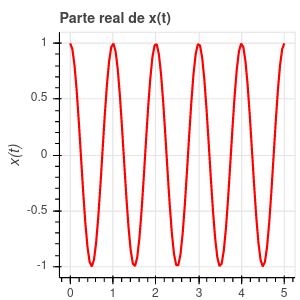
\includegraphics[width=\textwidth]{Figuras/exp_real.png}
    \end{minipage}
    \begin{minipage}{0.25\textwidth}
        \centering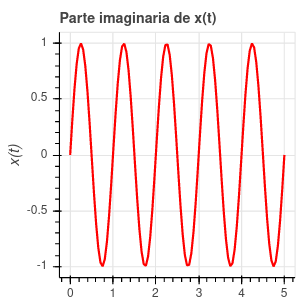
\includegraphics[width=\textwidth]{Figuras/exp_imag.png}
    \end{minipage}

    \begin{block}{{\scriptsize Fórmula de Euler}}\centering
        \scriptsize{$e^{j(\omega t+\phi)}=cos(\omega t+\phi)+j sin(\omega t+\phi)\Rightarrow \left\lbrace\begin{matrix}
            cos(\omega t+\phi)=\frac{e^{j(\omega t+\phi)}+e^{-j(\omega t+\phi)}}{2}\\
            sin(\omega t+\phi)=\frac{e^{j(\omega t+\phi)}-e^{-j(\omega t+\phi)}}{2j}\\
        \end{matrix}\right.$}
    \end{block}
\end{frame}


\begin{frame}
	\frametitle{Señales básicas: Exponencial Compleja}\centering

	\begin{itemize}
		\item \alert{Continua (Forma General):} $x(t)=C \mathsf{e}^{a t}$, con $C,a\in\mathbb{C}$
		\vspace{0.1cm}
		\begin{itemize}{\small
            \item $\left.\begin{matrix}C=|C|\mathsf{e}^{j\phi}\\a=r+j\omega\end{matrix}\right\rbrace \Rightarrow \color{blue}x(t)=|C| \mathsf{e}^{r t}\mathsf{e}^{\:j(\omega t+\phi)}\color{black}$
    %        \vspace{0.1cm}
            \item Sinusoidal multiplicada por exponencial
            \vspace{0.1cm}
            \item Decreciente ($r<0$), constante ($r=0$) o creciente ($r>0$)
            \vspace{0.1cm}
        }\end{itemize}
    \end{itemize}
    \begin{minipage}{0.25\textwidth}
        \centering\scriptsize{$r<0$}\\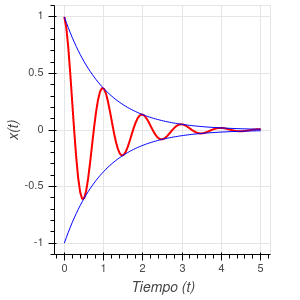
\includegraphics[width=\textwidth]{Figuras/exp_decreciente.png}
    \end{minipage}
    \begin{minipage}{0.25\textwidth}
        \centering\scriptsize{$r=0$}\\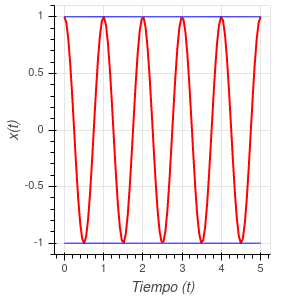
\includegraphics[width=\textwidth]{Figuras/exp_sin.png}
    \end{minipage}
    \begin{minipage}{0.25\textwidth}
        \centering\scriptsize{$r>0$}\\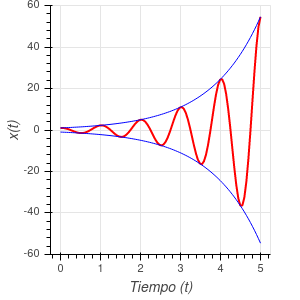
\includegraphics[width=\textwidth]{Figuras/exp_creciente.png}        
    \end{minipage}
    \begin{block}{{\scriptsize Fórmula de Euler}}\centering
        \scriptsize{$e^{j(\omega t+\phi)}=cos(\omega t+\phi)+j sin(\omega t+\phi)\Rightarrow \left\lbrace\begin{matrix}
            cos(\omega t+\phi)=\frac{e^{j(\omega t+\phi)}+e^{-j(\omega t+\phi)}}{2}\\
            sin(\omega t+\phi)=\frac{e^{j(\omega t+\phi)}-e^{-j(\omega t+\phi)}}{2j}\\
        \end{matrix}\right.$}
    \end{block}
\end{frame}


\begin{frame}
	\frametitle{Señales básicas: Exponencial Compleja}\centering
    \begin{itemize}
        \vspace{0.1cm}
		\item \alert{Discreta:} $x[n]=C \mathsf{e}^{j\omega n}$
		\begin{itemize}{\small
            \item \color{blue}$\omega=2\pi f$~\color{black} es la frecuencia en rad/muestra
            \vspace{0.1cm}
            \item \color{blue}$x[n]=x[n+N]$\color{black}, con $N=\frac{1}{f}=\frac{2\pi}{\omega}$ \color{red}sólo si \color{black}
            \vspace{0.1cm}
            \color{cyan}{\tiny $x[n+N]=C\mathsf{e}^{\:j\omega (n+N)}=C\mathsf{e}^{\:j(\omega n+\omega N)}=C\mathsf{e}^{\:j\omega n}\mathsf{e}^{\:j\omega N}=x[n]$\\
            \vspace{0.1cm}
            $\mathsf{e}^{\:j\omega N}=1\Rightarrow 2\pi f N=2\pi k \Rightarrow f=\frac{k}{N}$, para algún $N,k\in\mathbb{N}$\\
            Nota: $\frac{k}{N}$ es una fracción irreducible, en caso contrario $\frac{a}{b}=\frac{m\cdot k}{m\cdot N}=\frac{k}{N}$
            }\color{black}


            \vspace{0.1cm}
            \item \color{blue}$\omega_1\neq\omega_2 \Rightarrow x_1[n]\neq x_2[n]$\color{black}, \color{red}sólo para $0<\omega<2\pi\color{black}$\\
            \vspace{0.1cm}
            \color{cyan}{\scriptsize $\omega_k=\omega+2\pi k \Rightarrow$
            $C\mathsf{e}^{\:j(\omega + 2\pi k) n}=C\mathsf{e}^{\:j\omega n+j2\pi k n}=C\mathsf{e}^{\:j\omega n}\mathsf{e}^{\:j2\pi k n}=C\mathsf{e}^{\:j\omega n}$}\color{black}
            \vspace{0.1cm}
        }\end{itemize}
    \end{itemize}

    \begin{block}{{\scriptsize Fórmula de Euler}}
        \centering
        \scriptsize{$e^{j\omega n+\phi}=cos(\omega n+\phi)+j sin(\omega n+\phi)\Rightarrow \left\lbrace\begin{matrix}
            cos(\omega n+\phi)=\frac{e^{j(\omega n+\phi)}+e^{-j(\omega n+\phi)}}{2}\\
            sin(\omega n+\phi)=\frac{e^{j(\omega n+\phi)}-e^{-j(\omega n+\phi)}}{2j}\\
        \end{matrix}\right.$}
    \end{block}
\end{frame}


\begin{frame}
	\frametitle{Señales básicas: Exponencial Compleja}\centering
    \begin{itemize}{\scriptsize
        \vspace{0.1cm}
		\item \alert{Exponencial Discreta (sinusoidal):} $x[n]=C \alpha^n$, con $C,\alpha\in\mathbb{C}$
		\begin{itemize}{\scriptsize
            \item $\left.\begin{matrix}C=|C|e^{\phi}\\\alpha=|\alpha|e^{j\omega}\end{matrix}\right\rbrace \Rightarrow\color{blue}x(t)=|C||\alpha|^{n}e^{~j\omega n+\phi}\color{black}$
            \vspace{0.1cm}
            \item Decreciente ($0<\alpha<1$), constante ($\alpha=1$), o creciente ($\alpha>1$)
            \vspace{0.1cm}
        }\end{itemize}
    }\end{itemize}
    \begin{minipage}{0.25\textwidth}
        \centering\scriptsize{$0<|\alpha|<1$}\\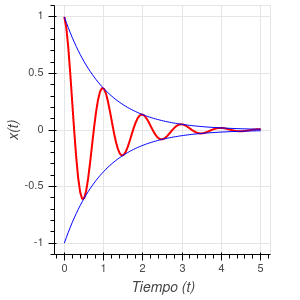
\includegraphics[width=\textwidth]{Figuras/exp_decreciente.png}
    \end{minipage}
    \begin{minipage}{0.25\textwidth}
        \centering\scriptsize{$|\alpha|=1$}\\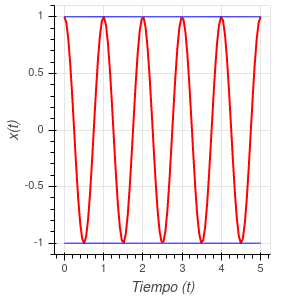
\includegraphics[width=\textwidth]{Figuras/exp_sin.png}
    \end{minipage}
    \begin{minipage}{0.25\textwidth}
        \centering\scriptsize{$|\alpha|>1$}\\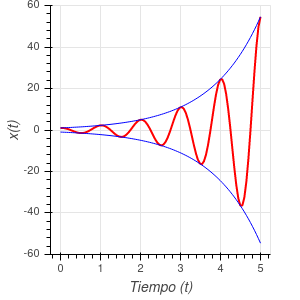
\includegraphics[width=\textwidth]{Figuras/exp_creciente.png}
    \end{minipage}

    \begin{block}{Fórmula de Euler}
        \centering
        \scriptsize{$e^{j\omega n+\phi}=cos(\omega n+\phi)+j sin(\omega n+\phi)\Rightarrow \begin{matrix}
            cos(\omega n+\phi)=\frac{e^{j\omega n+\phi}+e^{-j\omega n-\phi}}{2}\\
            sin(\omega n+\phi)=\frac{e^{j\omega n+\phi}-e^{-j\omega n-\phi}}{2}\\
        \end{matrix}$}
    \end{block}
\end{frame}

%%%%%%%%%%%%%%%%%%%%%%%%%%%%%%%%%%%%%%%%%%%%%%

\begin{frame}
	\frametitle{Señales básicas: Impulso}
	
	\begin{itemize}
        \item \alert{Continuo ($\delta$ de Dirac):} {\scriptsize \hspace{1cm}$\delta(t)=\left \{ \begin{array}{l} \infty \:\: \: \:t=0\\0 \:\: \:\: \forall t \neq0\end{array}\right .$}%
        \begin{columns}[c]
            \begin{column}{0.2\textwidth}\centering
                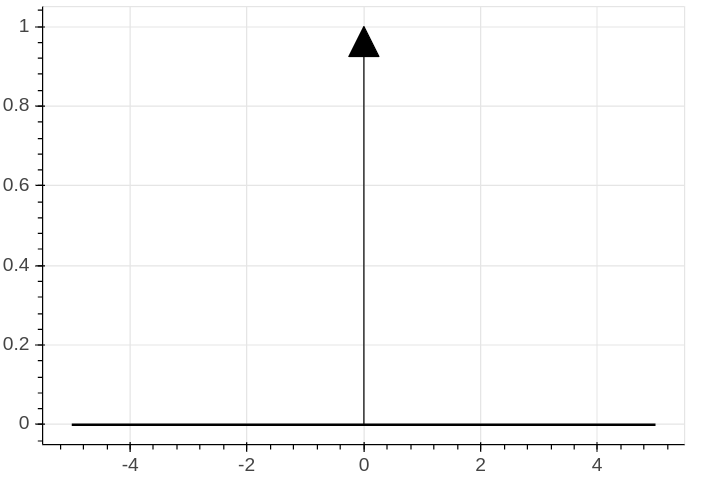
\includegraphics[width=4cm]{./Figuras/dirac}\\%
            \end{column}
            \hspace{0.3cm}
            \begin{column}{0.65\textwidth}
                {\scriptsize
                \begin{itemize}
                    {\scriptsize
                    \vspace{0.1cm}
                    \item Es un funcional:\\ \vspace{0.1cm}
                    $\int_{-\infty}^{\infty} f(t)\delta(t)dt=f(0)$\hspace{0.2cm}\color{olivegreen}$\int_{-\infty}^{\infty} f(t)\delta(t-t_0)dt=f(t_0)$\color{black}\\
                    \item Algunas propiedades:
                    $\int_{t_1}^{t_2} f(t)\delta(t-t_0)dt=\left\{\! \!\begin{array}{l}f(t_0)  \:\:\: t_1\!<t_0\!<t_2 \\ 0 \:\:\: c.c.    \end{array}\right .$
                    $\forall a\neq 0 \Rightarrow \delta(at)=\frac{\delta(t)}{|a|}$
                    $(x \ast \delta)(t) = \int_{-\infty}^\infty x(\tau)\delta(t-\tau)d\tau=x(t)$\\
                }\end{itemize}
                \vspace{0.2cm}
                \vspace{0.2cm}
            }\end{column}
        \end{columns}
        \vspace{-0.4cm}
        \item \alert{Discreto ($\delta$ de Kronecker):} {\scriptsize \hspace{0.5cm}$\delta(n)=\left \{ \begin{array}{l} 1\:\: \: \:n=0\\0 \:\: \:\: \forall n \neq0\end{array}\right .$}
        \begin{columns}[c]
            \begin{column}{0.22\textwidth}{\scriptsize
                \centering
                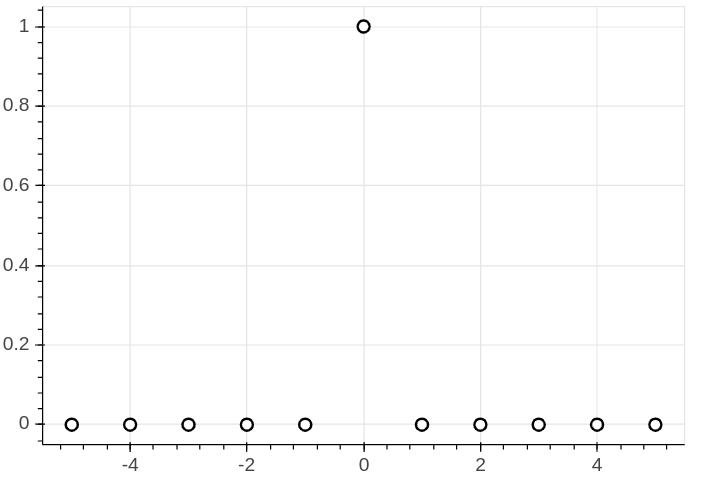
\includegraphics[width=4cm]{./Figuras/kronecker}\\%
            }\end{column}
            \begin{column}{0.65\textwidth}{\scriptsize
                \hspace{1.5cm}\color{olivegreen}$x[n]=\sum_{k=-\infty}^{\infty} x[k]\delta[k-n]$\color{black}\\
                \vspace{0.4cm}
                \hspace{1.5cm}$(x\! \ast\! \delta)[n] \!=\! \sum_{k=-\infty}^\infty x[k]\delta[n-k]=x[n]$
            }\end{column}
        \end{columns}
    \end{itemize}
\end{frame}
	
%%%%%%%%%%%%%%%%%%%%%%%%%%%%%%%%%%%%%%%%%%%%%%

\begin{frame}
\frametitle{Señales básicas: Escalón unitario}

\begin{itemize}

\begin{columns}[c]
    \begin{column}{7.0cm}
    
    \item \alert{Continuo:} $u(t)=\left \{ \begin{array}{l} 0 \:\: \: \:t<0\\1 \:\: \:\:  t \ge 0\end{array}\right .$

\vspace{0.1cm}

    
    \small Relación con el impulso:

\vspace{0.1cm}

$\delta(t)=\frac{du(t)}{dt}$

\vspace{0.1cm}

$u(t)=\int _{-\infty} ^t \delta(\tau)d\tau$

\vspace{0.1cm}

Convolución: $(x \ast u)(t)=\int _{-\infty} ^t x(\tau)d\tau $
    
    \end{column}
\hspace{-2.5cm}\begin{column}{5cm}
    \begin{figure}
\centering
\footnotesize
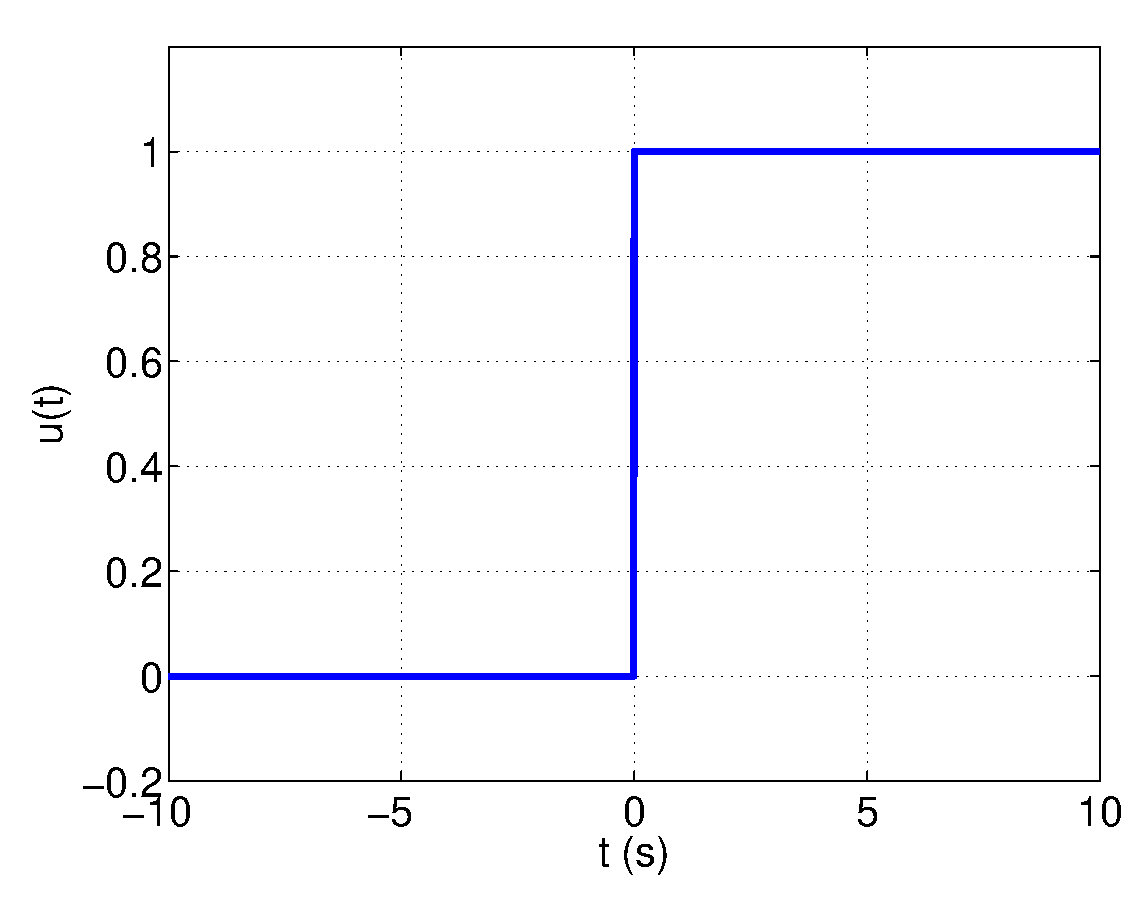
\includegraphics[width=4cm]{./Figuras/EscalonT.eps} 
\end{figure}
    \end{column}
    \end{columns}
    
\vspace{-0.2cm}

\hspace{1cm}\begin{columns}[c]
    \begin{column}{6.0cm}
                    \item \alert{Discreto:}  $u[n]=\left \{ \begin{array}{l} 0\:\: \: \:n<0\\1 \:\: \:\:  n \ge 0\end{array}\right .$
    
            \vspace{0.2cm}
    
    \small Relación con el impulso:

\vspace{0.2cm}

$\delta[n]=u[n]-u[n-1]$

\vspace{0.2cm}

$u[n]=\sum _{k=-\infty} ^n \delta[k]$
    
    \vspace{0.2cm}

Convolución: $(x\! \ast \! u)[n]\!=\!\sum _{k=-\infty} ^n x[k]$
    
    \end{column}
\hspace{-1.5cm}\begin{column}{5cm}
    \begin{figure}
\centering
\footnotesize
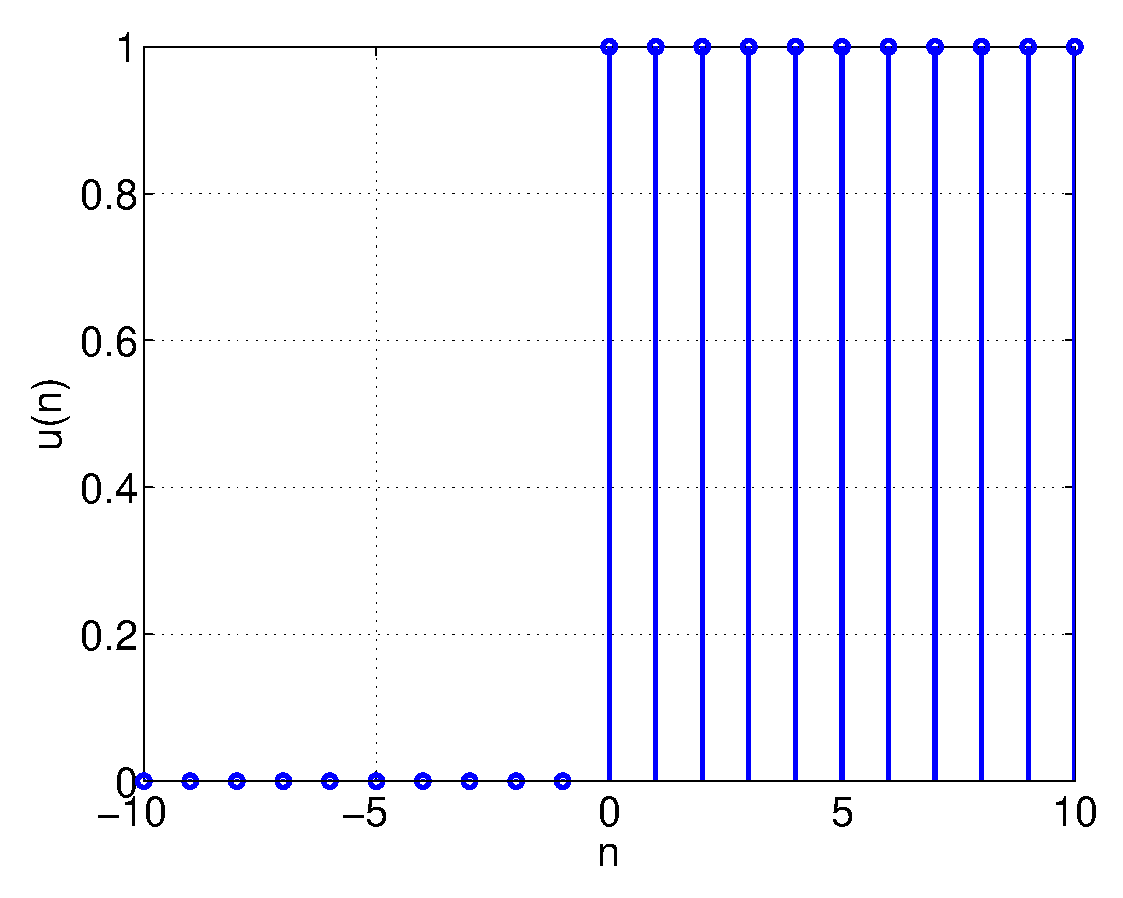
\includegraphics[width=4cm]{./Figuras/EscalonN.eps} 
\end{figure}
    \end{column}
    \end{columns}


\end{itemize}

\small El producto de cualquier señal $x(\cdot)$ por $u(\cdot)$ produce una señal causal.

\end{frame}

%%%%%%%%%%%%%%%%%%%%%%%%%%%%%%%%%%%%%%%%%%%%%%%
	
	
\begin{frame}
\frametitle{Señales básicas: Rampa}

\begin{itemize}

\begin{columns}[c]
    \begin{column}{7.0cm}
        \item \alert{Continuo:} $r(t)=\left \{ \begin{array}{l} 0 \\ t \end{array}\begin{array}{l}t<0 \\ t \ge 0\end{array}\right .$

\vspace{0.1cm}

    
    \small Relación con el escalón:

\vspace{0.1cm}

$u(t)=\frac{dr(t)}{dt}$

\vspace{0.1cm}

$r(t)=\int _{-\infty} ^t u(\tau)d\tau$

\vspace{0.1cm}

    
    \end{column}
\hspace{-2.5cm}\begin{column}{5cm}
    \begin{figure}
\centering
\footnotesize
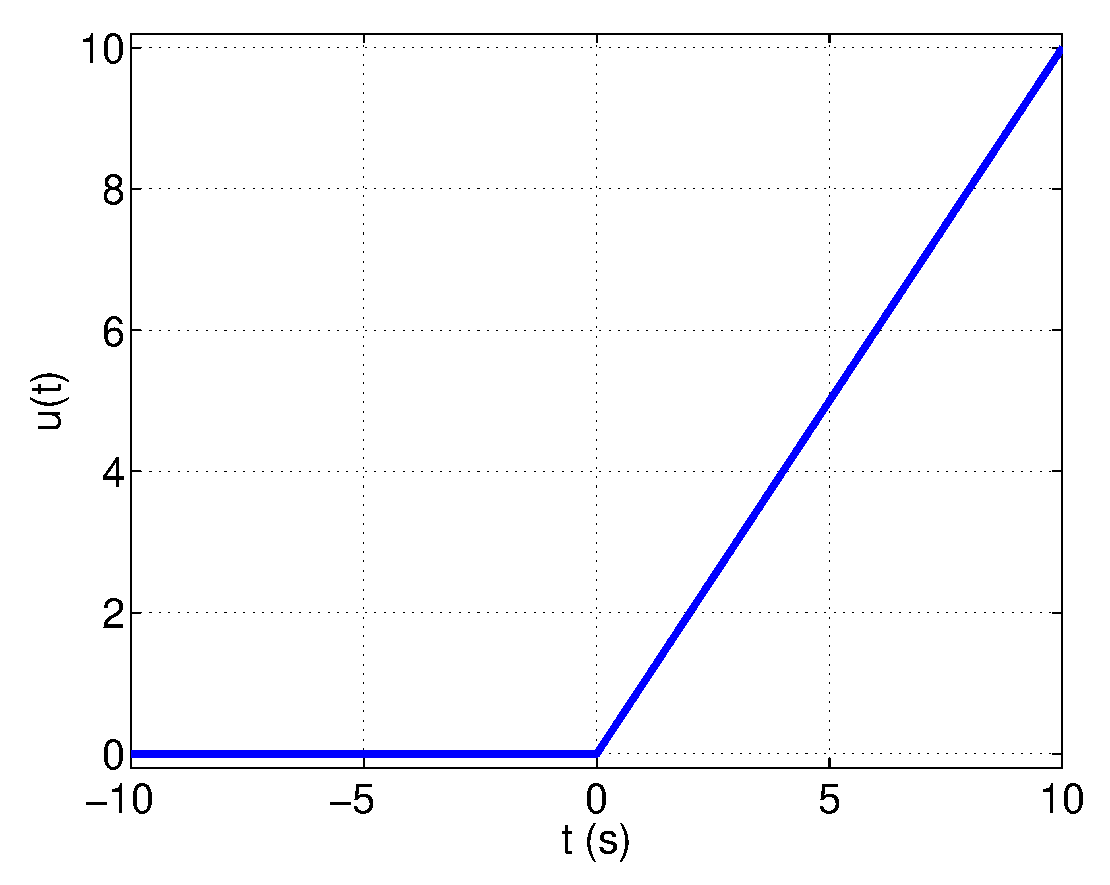
\includegraphics[width=4cm]{./Figuras/RampaT.eps} 
\end{figure}
    \end{column}
    \end{columns}
    
\vspace{-0.2cm}

\hspace{1cm}\begin{columns}[c]
    \begin{column}{6.0cm}
                    \item \alert{Discreto:}  $r[n]=\left \{ \begin{array}{l} 0 \\n+1\end{array}\begin{array}{l} n<0\\n \ge 0\end{array}\right .$
    
    
            \vspace{0.2cm}
    
    \small Relación con el escalón:

\vspace{0.2cm}

$u[n]=r[n]-r[n-1]$

\vspace{0.2cm}

$r[n]=\sum _{k=-\infty} ^n u[k]$
    
    \vspace{0.2cm}
    
    \end{column}
\hspace{-1.5cm}\begin{column}{5cm}
    \begin{figure}
\centering
\footnotesize
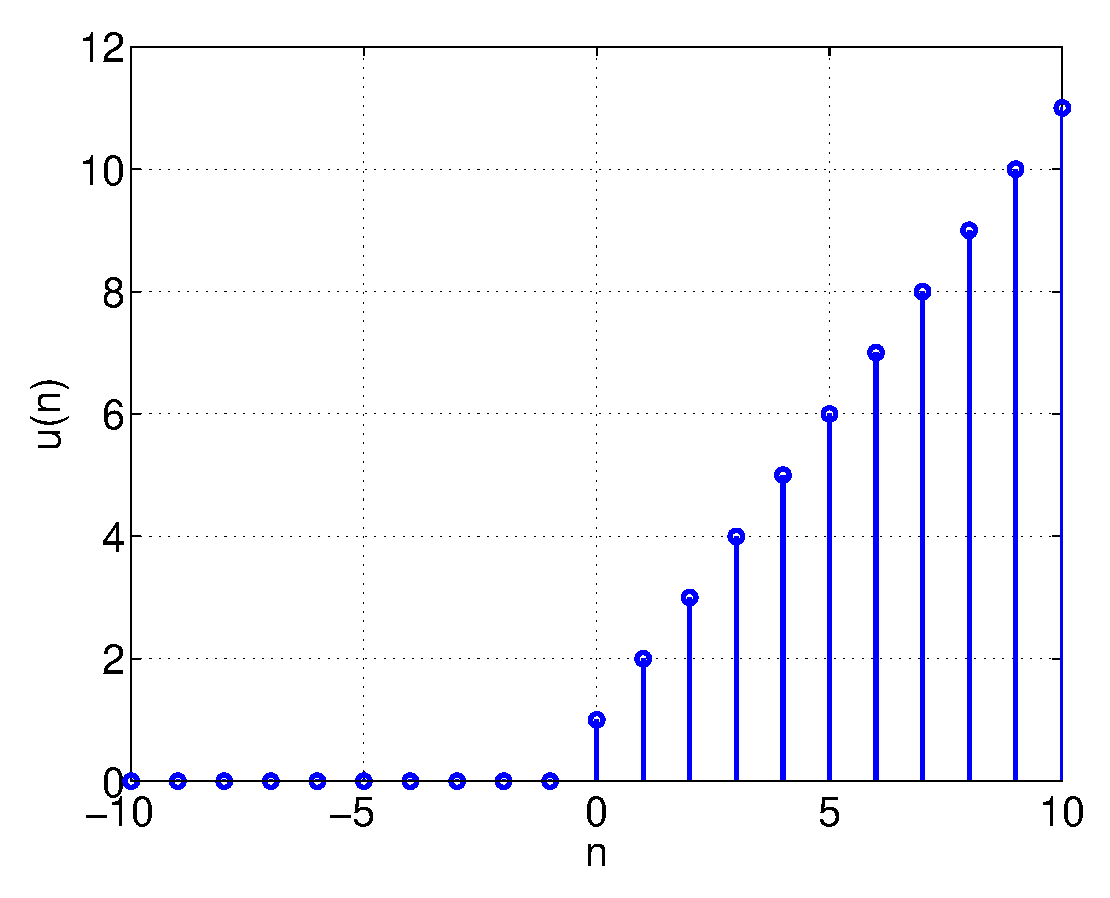
\includegraphics[width=4cm]{./Figuras/RampaN.eps} 
\end{figure}
    \end{column}
    \end{columns}


\end{itemize}


\end{frame}


%%%%%%%%%%%%%%%%%%%%%%%%%%%%%%%%%%%%%%%%%%%%%%

\begin{frame}\frametitle{Señales básicas: Pulsos}

    \begin{itemize}
        \begin{columns}[c]
            \begin{column}{5cm}
            \item \alert{Pulso rectangular}
                \vspace{0.3cm}
                $\Pi(t)=\left \{ \begin{array}{l} 1 \:\: \: \:|t| \le \frac{1}{2}\\0 \:\: \:\:  |t| > \frac{1}{2}\end{array}\right .$            
                \begin{figure}
                    \centering
                    \footnotesize
                    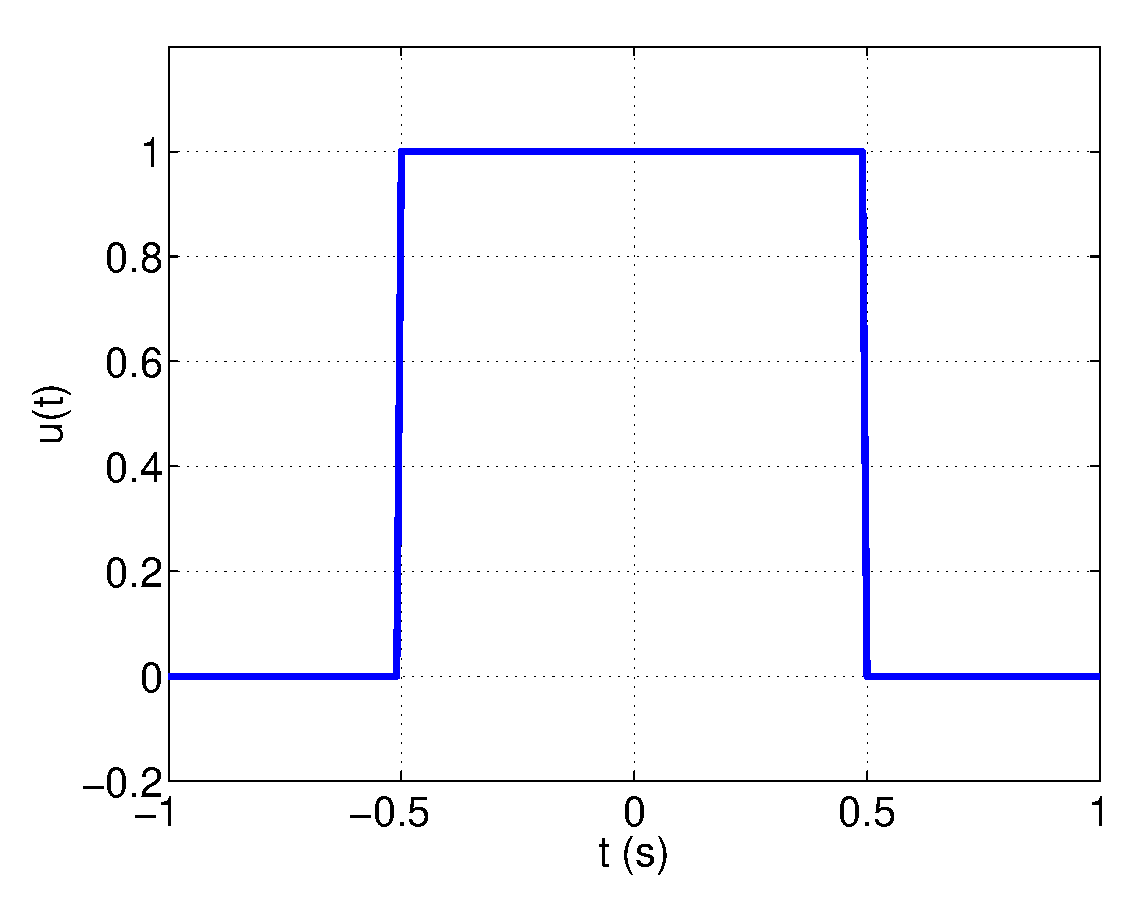
\includegraphics[width=5cm]{./Figuras/PulsoRect.eps} 
                \end{figure}
            \end{column}
            \begin{column}{5.cm}
                \item \alert{Pulso triangular}
                \vspace{0.3cm}
                $\Lambda(t)=\left \{\!\! \begin{array}{l} t+1 \:\: \: \:-1 \le t \le 0\\1-t \:\: \:\: \:\: \:\: \: 0 \le t \le 1\end{array}\right .$            
                \begin{figure}
                    \centering
                    \footnotesize
                    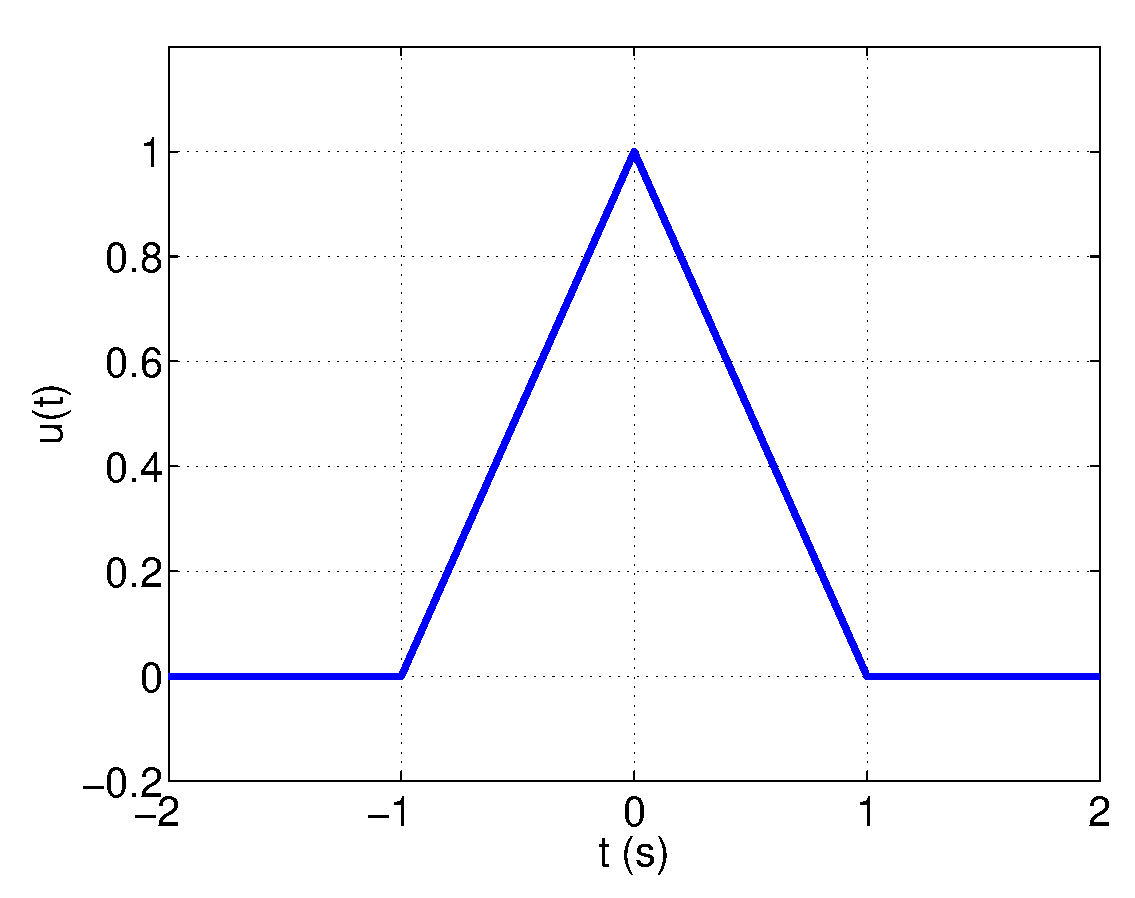
\includegraphics[width=5cm]{./Figuras/PulsoTri.eps} 
                \end{figure}
            \end{column}
        \end{columns}
    \end{itemize}
\end{frame}

%%%%%%%%%%%%%%%%%%%%%%%%%%%%%%%%%%%%%%%%%%%%%%%%%%%%%%


\begin{frame}
\frametitle{Señales básicas: muestreo, sinc, signo }

\vspace{-0.4cm}

\begin{itemize}



\begin{columns}[c]
    \begin{column}{4.5cm}
    
    \vspace{-0.8cm}
    
    \item \alert{Muestreo}

\vspace{0.3cm}

        $Sa(t)=\left \{ \begin{array}{l} \frac{sin(t)}{t} \:\: \: \:t \neq 0\\1 \:\: \:\: \:\: \:\: \:\: \:t=0\end{array}\right .$
        
            \item \alert{Sinc}

\vspace{0.3cm}

        $sinc(t)=\left \{\!\! \begin{array}{l} \frac{sin(\pi t)}{\pi t} \:\: \: \: t \ne 0 \\1 \:\: \:\:  \:\: \:\: \:\: \:\:  \: t=0\end{array}\right .$
    
    
    \vspace{0.7cm}
    
    
    \item \alert{Signo}

\vspace{0.3cm}

        $sgn(t)=\left \{\!\! \begin{array}{l} 1 \:\: \: \: \:\: \:\:t > 0 \\-1 \:\: \:\:   t<0 \\ 0  \:\: \:\:  \:\: \:\: t=0\end{array}\right .$


    
    \end{column}
\hspace{-0.5cm}	\begin{column}{4.5cm}
    
    \vspace{0.6cm}
            \begin{figure}
\centering
\footnotesize
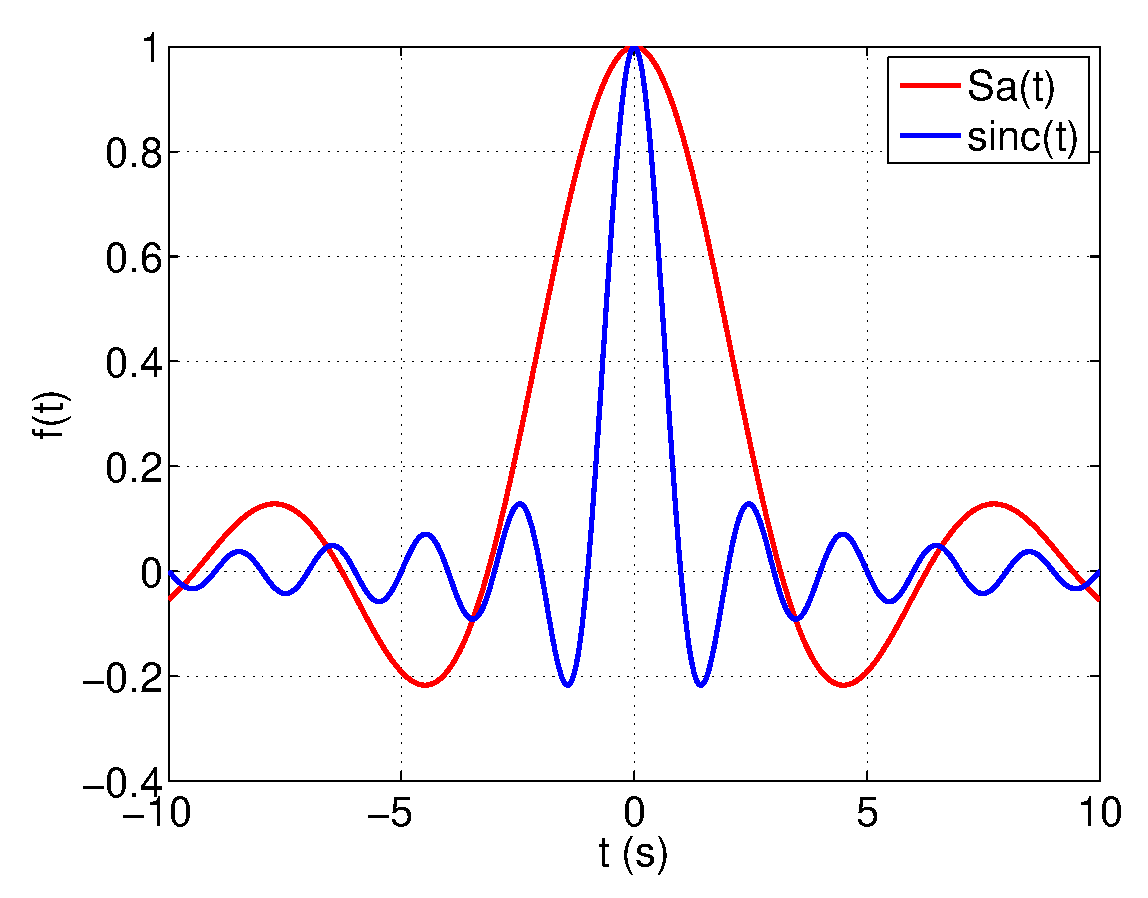
\includegraphics[width=4.5cm]{./Figuras/MuestreoSinc.eps} 
\end{figure}

            \begin{figure}
\centering
\footnotesize
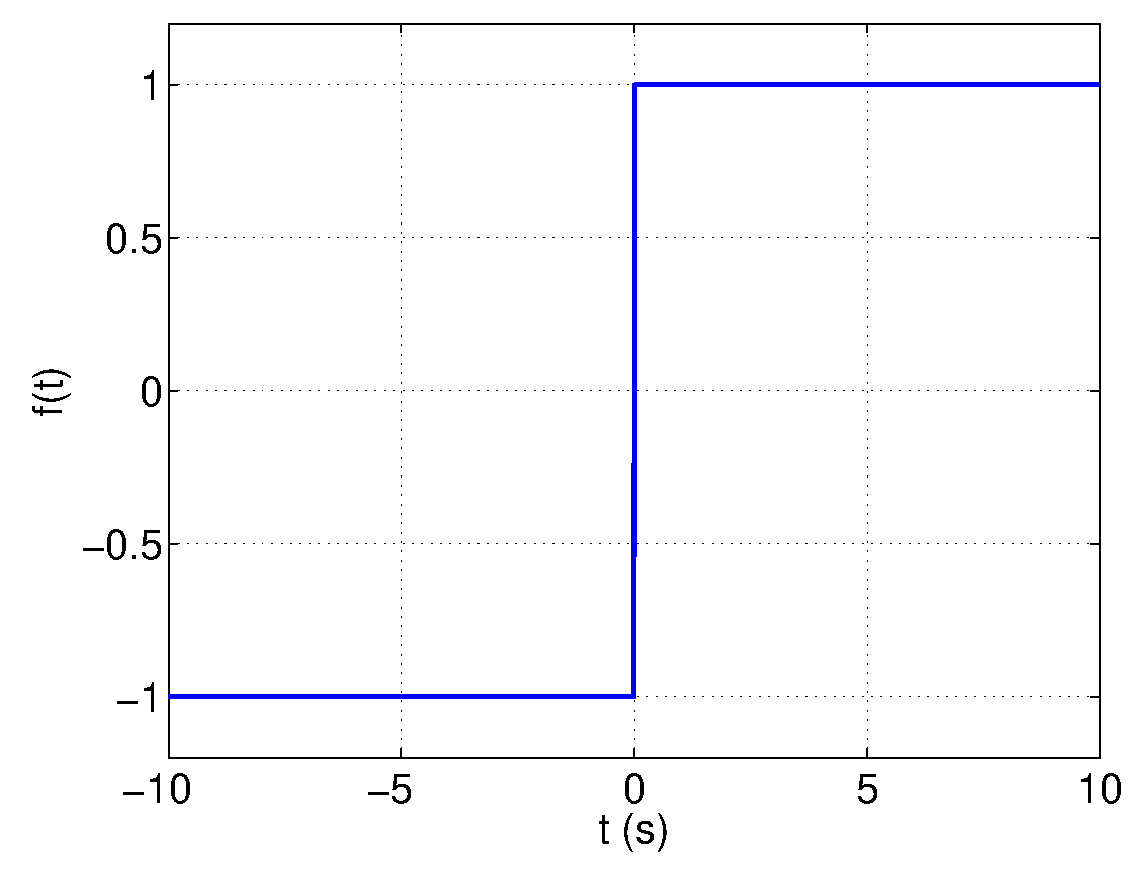
\includegraphics[width=4.5cm]{./Figuras/Signo.eps} 
\end{figure}

    
    \end{column}
    \end{columns}


\end{itemize}





\end{frame}

%%%%%%%%%%%%%%%%%%%%%%%%%%%%

\begin{frame}
\frametitle{Señales básicas: ondas  }

\begin{itemize}

\begin{columns}[c]
    \begin{column}{4.5cm}
    
    \item \alert{Onda cuadrada}

\vspace{0.3cm}

    
            
            \begin{figure}
\centering
\footnotesize
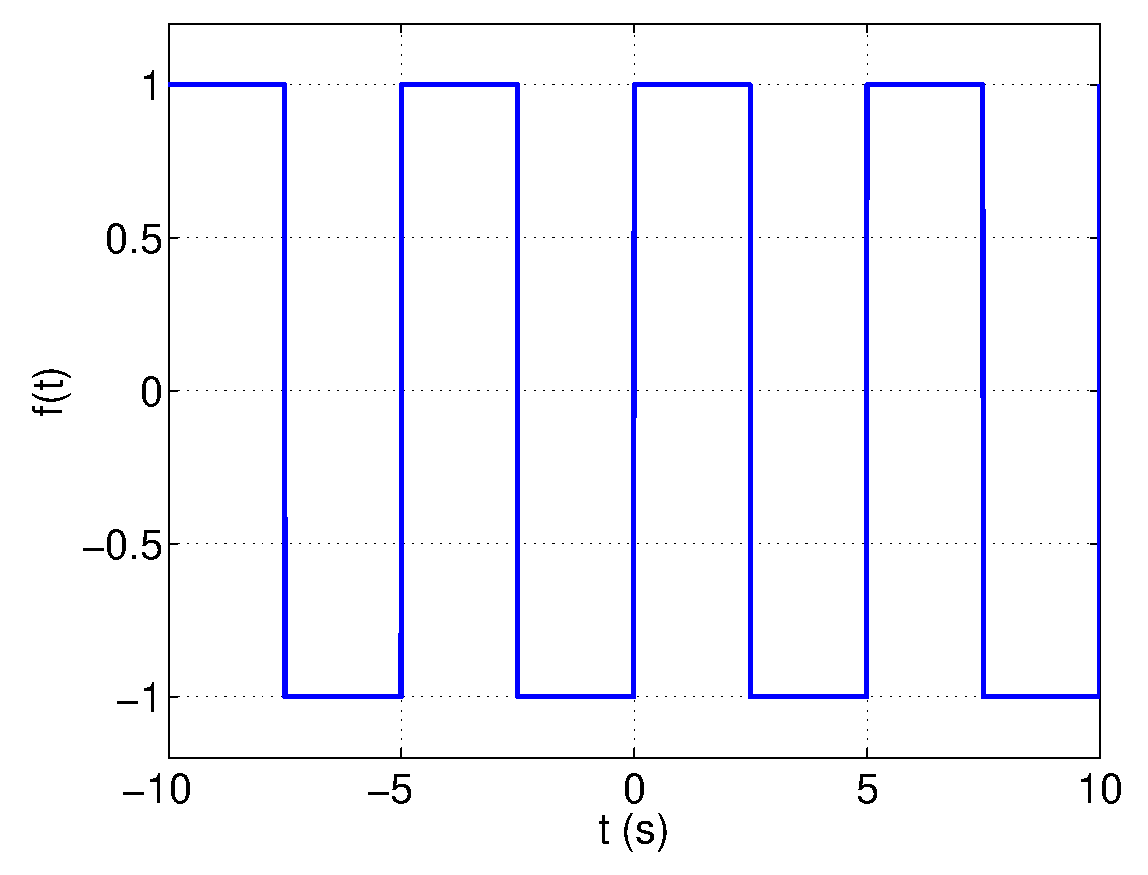
\includegraphics[width=4.5cm]{./Figuras/Square.eps} 

$T=5$
\end{figure}
    
    
    

    
    \end{column}
\hspace{-0.5cm}	\begin{column}{4.5cm}
    
        \item \alert{Onda triangular}

\vspace{0.3cm}




            \begin{figure}
\centering
\footnotesize
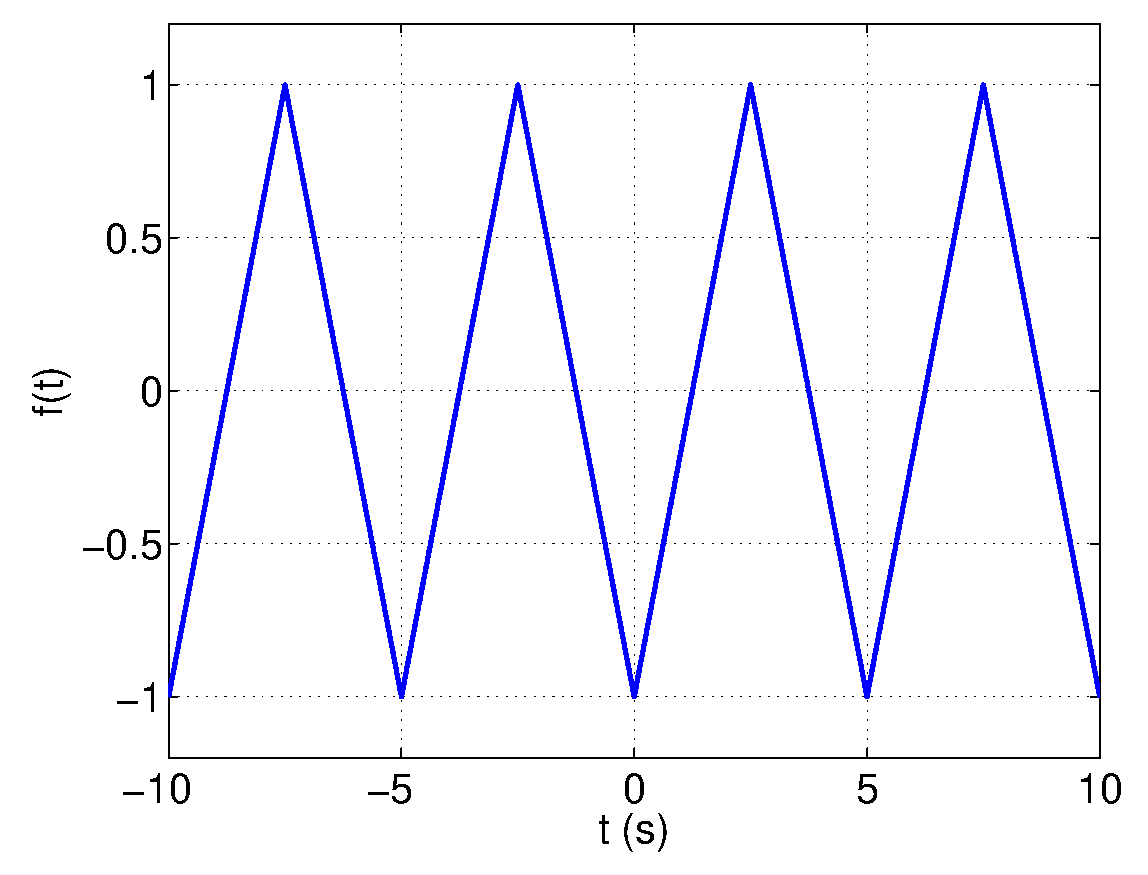
\includegraphics[width=4.5cm]{./Figuras/Triangular.eps} 

$T=5$
\end{figure}

    
    \end{column}
    \end{columns}


\end{itemize}

\end{frame}

\begin{frame}
\frametitle{Señales básicas: chirp  }

\begin{itemize}

\begin{columns}[c]

\hspace{-0.5cm}	\begin{column}{4.5cm}
    
        \item \alert{Chirp de variaci\'{o}n lineal}

\vspace{0.3cm}




\begin{figure}
    \centering
\footnotesize
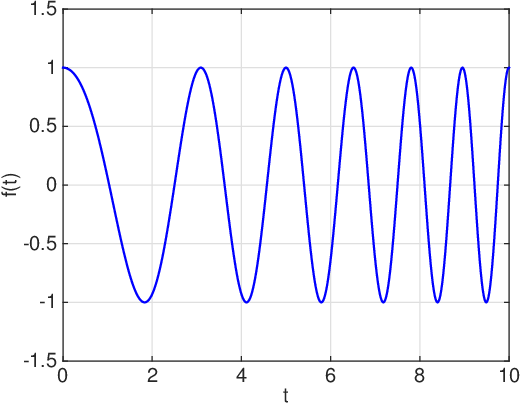
\includegraphics[width=4.5cm]{./Figuras/chirp} 

$f_{t=0}=0.2$ y $f_{t=10}=1$ 
\end{figure}

    
    \end{column}
    \end{columns}


\end{itemize}

\end{frame}



\section{Sistemas}
\subsection{Tipos de Sistemas}

\begin{frame}
  \frametitle{Tipos de Sistemas I}

  \vspace{-0,3cm}

  \begin{figure}
    \centering
    \small
    \begin{tikzpicture}
      \node[bloque,minimum width=15mm] (T) {T};
      \node (x) [left=of T] {};
      \node (y) [right=of T] {};
      \draw[arrow,->] (x.east) -- (T.west) node [midway,above] {$x(\cdot)$};
      \draw[arrow,->] (T.east) -- (y.west) node [midway,above] {$y(\cdot)$};
    \end{tikzpicture}
  \end{figure}
  \vspace{-0,25cm}
  \begin{itemize}
    \item <1-> Seg\'{u}n el n\'{u}mero de variables de entrada y de salida:
    \begin{itemize}
      \item \color{olivegreen}{SISO }\color{black}  (Single-Input, Single-Output): 1 variable de entrada, 1 variable de salida
      \item \alert{MIMO} (Multiple-Input, Multiple-Output): multiples variables de entrada, multiples variables de salida
      \item \alert{SIMO} (Single-Input, Multiple-Output): 1 variable de entrada, multiples variables de salida
      \item \alert{MISO} (Multiple-Input, Single-Output): multiples variables de entrada, 1 variable de salida
      \item \alert{Aut\'{o}nomo}:  sistema sin entradas de control
    \end{itemize}

    \item <2-> Según las características de la variable independiente:
    \begin{itemize}
      \item \alert{Sistemas Continuos}: admite/devuelve señales continuas
      \item \alert{Sistemas Discretos}: admite/devuelve señales discretas
      \item \alert{Conversores}: Admiten señales continuas/discretas y devuelven señales discretas/continuas
    \end{itemize}
  \end{itemize}

  \vspace{-0.4cm}

\end{frame}

%%%%%%%%%%%%%%%%%%%%%%%%%%%%%%%%%%%%%%%%%%%%

\begin{frame}
  \frametitle{Tipos de Sistemas II}

  \vspace{-0,3cm}

  \begin{figure}
    \centering
    \small
    \begin{tikzpicture}
      \node[bloque,minimum width=15mm] (T) {T};
      \node (x) [left=of T] {};
      \node (y) [right=of T] {};
      \draw[arrow,->] (x.east) -- (T.west) node [midway,above] {$x(\cdot)$};
      \draw[arrow,->] (T.east) -- (y.west) node [midway,above] {$y(\cdot)$};
    \end{tikzpicture}
  \end{figure}

  \vspace{-0.25cm}

  \begin{itemize}
    \item <1-> Seg\'{u}n la existencia o no de procesos aleatorios:
    \begin{itemize}
      \item \alert{Sistemas Deterministas}: no hay procesos aleatorios involucrados, por lo que la respuesta del sistema ante la mismas entradas es siempre la misma.
      \item \alert{Sistemas Estoc\'{a}sticos}: hay procesos aleatorios involucrados, por lo que la respuesta del sistema ante la mismas entradas depende del experimento.
    \end{itemize}

    \item <2-> Causales/no causales:
    \begin{itemize}
      \item \color{olivegreen}{Sistemas Causales}\color{black}: La salida del sistema en un instante únicamente depende de las entradas hasta dicho instante de tiempo. 

  \vspace{0.2cm}

     \hspace{0.4cm} $y(t)=\bm{T} [ \:x(\tau)|\tau<=t\: ] \: \:$       ó          $\: \:y[n]=\bm{T}[\: x[k]|k<=n\:]$ 
     
     \vspace{0.2cm}
     
      \item \alert{Sistemas No Causales}: La salida del sistema en un instante depende de la entrada en instantes posteriores. No es físicamente realizable. 
    \end{itemize}

  \end{itemize}

\vspace{-0.4cm}

\end{frame}

% %%%%%%%%%%%%%%%%%%%%%%%

\begin{frame}
\frametitle{Tipos de Sistemas III}

\vspace{-0,1cm}

\begin{figure}
  \centering
  \small
  \begin{tikzpicture}
    \node[bloque,minimum width=15mm] (T) {T};
    \node (x) [left=of T] {};
    \node (y) [right=of T] {};
    \draw[arrow,->] (x.east) -- (T.west) node [midway,above] {$x(\cdot)$};
    \draw[arrow,->] (T.east) -- (y.west) node [midway,above] {$y(\cdot)$};
  \end{tikzpicture}
  \end{figure}

  \vspace{-0.25cm}
  \begin{itemize}
    \item <1-> Respecto a la memoria del sistema:
    \begin{itemize}
      \item \alert{Sistemas Estáticos}: La salida del sistema en un instante depende únicamente de la entrada en dicho instante. 
  
      \vspace{0.1cm}
      \hspace{1cm}    $y(t)=\bm{T}[\:x(t)\:] \: \:$       ó          $\: \:y(n)=\bm{T}[\:x[n]\:]$ 
  
      \vspace{0.1cm}    
      \item \color{olivegreen}{Sistemas Dinámicos}\color{black}: La salida del sistema en un instante depende de la historia pasada del sistema. Los sistemas dinámicos continuos se pueden modelar con una ecuación diferencial. Los discretos con una ecuación en diferencias.

      \vspace{0.1cm}

      $y(t)=\bm{T}[\:x(\tau) | \tau \subseteq \mathbb{R} \le t\:] \: \:$       ó          $\: \:y(n)=\bm{T}[\:x[k] | k \subseteq \mathbb{Z} \le n\:]$
      \vspace{0.1cm}
 
    \end{itemize}

    \item <2-> Estable/inestable:
    \begin{itemize}
      \item \color{olivegreen}{Sistemas Estables}\color{black}: cuando responde con una salida acotada en amplitud ante cualquier entrada acotada (BIBO-estable: bounded-input, bounded-output). 

      \vspace{0.1cm}

      \hspace{1.8cm} $|x(\cdot)|< B_1  \rightarrow  |y(\cdot)|< B_2$  
     
      \vspace{0.1cm}
      \item \alert{Sistemas Inestables}\color{black}: cuando no cumplen la propiedad anterior. 


    \end{itemize}

%\item <1-> Invertibles/no invertibles:
%\begin{itemize}
%\item \alert{Sistemas Invertibles}\color{black}: en los que  existe una función $\bm{T}^{-1}[\cdot]$ que permite recuperar la entrada a partir de la salida. 

%  \vspace{0.1cm}

%     \hspace{1.8cm} $x(\cdot)=\bm{T}^{-1} [\: \bm{T}[\:x(\cdot)\: ]  \: ]$  
     
% \vspace{0.1cm}
     

     
%\item \alert{Sistemas No Invertibles}: en los que no existe la función $\bm{T}^{-1}[\cdot]$.
%\end{itemize}
  \end{itemize}
\end{frame}

% %%%%%%%%%%%%%%%%%




\begin{frame}
  \frametitle{Tipos de Sistemas IV}

  \vspace{-0.4cm}

  \begin{columns}[c]
    \hspace{-1.8cm}\begin{column}{12cm}
      \small 
      \begin{itemize}
        \item <1-> Sistemas lineales/no lineales:
        \begin{itemize}
          \item \color{olivegreen}{Sistemas Lineales}\color{black}: Los que cumplen el principio de superposición, i.e. la respuesta del sistema producido por varias fuentes excitadoras a la vez es la suma de las respuestas producidas por las fuentes individualmente.
          \vspace{0.1cm}
          $\bm{T}[\:\alpha x_1(\cdot)+\beta x_2(\cdot)\:]=\alpha \bm{T}[\:x_1(\cdot)\:] + \beta \bm{T}[\: x_2(\cdot) \:] =\alpha y_1(\cdot)+ \beta y_2(\cdot)$
          \vspace{0.1cm}
          \item \alert{Sistemas No Lineales}: Los que no cumplen el principio de superposición. Los sistemas reales son sistemas no lineales, aunque pueden ser tratados como sistemas lineales en torno a un determinado punto de operaci\'{o}n.
        \end{itemize}
      \end{itemize}
    \end{column}
    \hspace{-7cm}\begin{column}{4cm}
      \vspace{-3.75cm}
      \small
      \begin{tikzpicture}
        \node[bloque,minimum width=15mm] (T) {T};
        \node (x) [left=of T] {$x(\cdot)$};
        \node (y) [right=of T] {$y(\cdot)$};
        \draw[arrow,->] (x.east) -- (T.west);
        \draw[arrow,->] (T.east) -- (y.west);
      \end{tikzpicture}
    \end{column}
  \end{columns}
  \vspace{0.2cm}
  \begin{columns}[c]
    \begin{column}{4cm}
      \includegraphics[width=3.8cm]{./Figuras/FigLT1.eps} 
    \end{column}
    \begin{column}{4cm}
      \includegraphics[width=3.8cm]{./Figuras/FigLT2.eps} 
    \end{column}
    \begin{column}{4cm}
      \includegraphics[width=3.8cm]{./Figuras/FigLT3.eps} 
    \end{column}
  \end{columns}
\end{frame}

%%%%%%%%%%%%%%%%%%%%%%%%%%%%%%%%

\begin{frame}
  \frametitle{Tipos de Sistemas V}
  \small
  \vspace{-0.4cm}

  \begin{columns}[c]
    \hspace{-0.2cm}\begin{column}{12cm}
      \begin{itemize}
        \item <1-> Sistemas temporalmente invariantes/no invariantes:
        \vspace{-0.2cm}
        \begin{itemize}
          \item \color{olivegreen}{Sistemas Temporalmente  Invariantes}\color{black}: Aquellos en los que su relación entrada-salida es invariante en el tiempo (a una entrada desplazada temporalmente le corresponde la misma salida desplazada el mismo valor).
          \vspace{0.1cm}
          $\bm{T}[\: x(t)\:]=y(t) \rightarrow \bm{T}[\: x(t-t_0)\:]=y(t-t_0)$
          \vspace{0.1cm}
          $\bm{T}[\: x[n]\:]=y(n) \rightarrow \bm{T}[\: x(n-N_0)\:]=y(n-N_0)$
          \vspace{0.1cm}
          \item \alert{Sistemas Temporalmente No  Invariantes}: Los que no cumplen la propiedad anterior.
      \end{itemize}

      \begin{columns}[c]
        \begin{column}{4cm}
          \includegraphics[width=4cm]{./Figuras/FigLT1B.eps} 
        \end{column}
        \begin{column}{4cm}
          \includegraphics[width=4cm]{./Figuras/FigLT2B.eps} 
        \end{column}
      \end{columns}

      \vspace{-0.2cm}
      \item \color{olivegreen}{Sistemas Lineales Temporalmente Invariantes}: Sistemas LTI
      \end{itemize}
    \end{column}
    \hspace{-3.0cm}\begin{column}{4cm}
      \vspace{7.25cm}
      \small
      \begin{tikzpicture}[scale=0.8,every node/.style={scale=0.8}]
        \node[bloque,minimum width=15mm] (T) {T};
        \node (x) [left=of T] {};
        \node (y) [right=of T] {};
        \draw[arrow,->] (x.east) -- (T.west) node [midway,above] {$x(\cdot)$};
        \draw[arrow,->] (T.east) -- (y.west) node [midway,above] {$y(\cdot)$};
      \end{tikzpicture}
    \end{column}
  \end{columns}

\end{frame}
\subsection{Sistemas LTI}

\begin{frame}
\frametitle{Sistemas LTI}

\vspace{-0,3cm}

  \begin{figure}
    \centering
    \small
    \begin{tikzpicture}
      \node[bloque,minimum width=15mm] (T) {LTI};
      \node (x) [left=of T] {};
      \node (y) [right=of T] {};
      \draw[arrow,->] (x.east) -- (T.west) node [midway,above] {$x(\cdot)$};
      \draw[arrow,->] (T.east) -- (y.west) node [midway,above] {$y(\cdot)$};
    \end{tikzpicture}
  \end{figure}

  \begin{itemize}
    \item <1-> Constituyen una clase de sistemas muy importantes en procesamiento de señales, control de sistemas, teoría de la comunicación.

    \item Características más relevantes:

    \begin{itemize}

      \item <1-> La respuesta de un sistema LTI a una entrada puede obtenerse como la \alert{convolución} de la entrada con la respuesta del sistema a la entrada impulso unitario.

      \item <1-> Las \alert{transformadas} de Laplace, Z, Fourier \alert{de la convolución es el producto de las transformadas}. 

      \item Por lo tanto, podemos calcular la respuesta de los sistemas LTI ante una entrada a partir del producto de la transformada de la entrada y de la transformada del sistema. 

    \end{itemize}

  \end{itemize}

  \vspace{-0.4cm}

\end{frame}

%%%%%%%%%%%%%%%%%%%%%%%%%%%%%%%%%%%%%%%%%%%%


\begin{frame}
\frametitle{Respuesta temporal sistema LTI}

\vspace{-0,3cm}


\begin{itemize}
\item <1-> \alert{Sistemas Continuos}:

\begin{itemize}
\item Respuesta al impulso (función ponderatriz):   $\bm{T}[\delta(t)]=h(t)$
	
	\vspace{0,1cm}
	
\item Respuesta a una entrada arbitraria:

\vspace{0,2cm}

\footnotesize $\begin{array}{ll}\color{red}\!\!\bm{T}[x(t)]\color{black}\!\!\!\!\!\!&=\bm{T}[(x\!*\!\delta)(t)]\!=\!\bm{T}[\int_{-\infty}^{\infty} \! x(\tau)\delta({t\!-\!\tau})d\tau] \!=\!\int_{-\infty}^{\infty}\bm{T}[x(\tau)\delta({t\!-\!\tau})]d\tau \!=\\ [0.2cm]  & =\int_{-\infty}^{\infty} x(\tau) \bm{T}[\delta({t\!-\!\tau})]d\tau  =\int_{-\infty}^{\infty} x(\tau)  h(t\!-\!\tau) d\tau \color{red}= (x*h)(t)\color{black} \end{array}$


\end{itemize}


\item <2-> \alert{Sistemas Discretos}:

\begin{itemize}
\item Respuesta al impulso (función ponderatriz):   $\bm{T}[\delta(n)]=h(n)$
	
	\vspace{0,1cm}
	
\item  Respuesta a una entrada arbitraria:

\vspace{0,1cm}

\footnotesize $\begin{array}{ll}\color{red}\!\!\bm{T}[x(n)]\color{black}\!\!\!\!\!\!&=\!\bm{T}[(x\!*\!\delta)(n)]\!=\!\bm{T}[\sum_{k=-\infty}^{\infty} \! x(k)\delta({n\!-\!k})] \!=\!\!\sum_{k=-\infty}^{\infty}\! \!\bm{T}[x(k)\delta({n\!-\!k})]\!=\\ [0.2cm]  & =\!\sum_{k=-\infty}^{\infty} x(k) \bm{T}[\delta({n\!-\!k})]  \!=\!\sum_{k=-\infty}^{\infty} x(k)  h(n\!-\!k) \color{red} \!=\! (x\!*\!h)(n)\color{black} \end{array}$

\vspace{0,2cm}
\end{itemize}


\item <3-> \small La respuesta de un  sistema LTI a cualquier entrada $x(\cdot)$ se puede calcular como la convolución de la entrada y la respuesta del sistema a la entrada impulso $h(\cdot)$.

\vspace{0,1cm}

\hspace{2cm} \alert{$h(\cdot)=\bm{T}[\delta(\cdot)]  \rightarrow  \bm{T}[x(\cdot)]=(x* h)(\cdot)$}


\end{itemize}


\end{frame}

%%%%%%%%%%%%%%%%%%%%%%%%%%%%%%%%%%%%%%%%%%%%


\begin{frame}
\frametitle{Sistemas LTI continuos I}

\vspace{-0,3cm}


\begin{itemize}
\item <1-> \alert{Transformada de Laplace (TL)}:

\begin{itemize}
\item Bilateral:    $\mathcal{L}{[x(t)]}\!=\!X(s)\!=\! \int_{-\infty}^{\infty} \! \!x(t) e^{-t s} dt \:$ con   $s \in \mathbb{C}$


\vspace{0.1cm}

\item \color{olivegreen} Unilateral:    $\mathcal{L}{[x(t)]}\!=\!X(s)\!= \!\int_{0}^{\infty} \! \! x(t) e^{-t s}dt  \:$ con   $s \in \mathbb{C}$, $x(t)$ causal \color{black}

\vspace{-0.4cm}

\end{itemize}

\item <2-> \alert{Propiedades} (similares, se diferencian en las condiciones iniciales que aparecen en las derivadas):

\begin{itemize}
\item Linealidad : $\mathcal{L}[\alpha x_1(t)+\beta  x_2(t)]=\alpha \mathcal{L}[x_1(t)]+\beta \mathcal{L}[x_2(t)]$
\vspace{0.2cm}
\item Desplazamiento temporal: $\mathcal{L}[x(t-t_0)]=e^{-st_0} \mathcal{L}[x(t)]$
\vspace{0.2cm}
\item Derivada: $\mathcal{L}[\frac {dx(t)}{dt}]=s \mathcal{L}[x(t)]\color{olivegreen}-x(0)\color{black}$
\vspace{0.2cm}
\item Convolución: $\mathcal{L}[{(x*y)(t)}]= \mathcal{L}[x(t)]\mathcal{L}[y(t)]$
\end{itemize}

\item <3-> \alert{TL de la respuesta del sistema}:

\vspace{0.2cm}

\footnotesize $\mathcal{L}[ y(t)]\!=\!\mathcal{L}[ \bm T[{(x)(t)}]\!=\!\mathcal{L}[{(x*h)(t)}]\!=\!\mathcal{L}[{x(t)}]\mathcal{L}[{h(t)}]   \leftrightarrow     Y(s)\!=\!H(s)X(s)$  

\vspace{0.2cm}

La respuesta de un sistema LTI continuo a una entrada se puede calcular a partir de la TL inversa del producto de la TL de la señal y de la TL de la respuesta del sistema a la entrada impulso. 
\end{itemize}

%%%%%%%%%%%%%%%%%%%%%%%%%%%%%%%%%%%%%%%%%%%%%%%%%%%%%%%%%%%%%%%%%%%%%%%%

\end{frame}

\begin{frame}
\frametitle{Sistemas LTI continuos II}

\vspace{-0,3cm}


\begin{itemize}

\item <1-> \alert{TL de la respuesta del sistema}:

\vspace{0.2cm}

\hspace{1cm}{\footnotesize $\mathcal{L}[ y(t)]\!=\!\mathcal{L}[{x(t)}]\mathcal{L}[{h(t)}]   \leftrightarrow     Y(s)\!=\!H(s)X(s)$  }

\vspace{0.2cm}

\item <2-> \alert{Ecuación diferencial de un sistema LTI continuo:}

\vspace{0.2cm}


\hspace{0.5cm} {\footnotesize $\sum_{k=0}^N {a_k \frac{d^k y(t)}{dt}}=\sum_{k=0}^M {b_k \frac{d^k x(t)}{dt}}$   $\buildrel TL \over  \longrightarrow$   $\sum_{k=0}^N a_k s^k Y(s)=\sum_{k=0}^M b_k s^k X(s)  \rightarrow $

\vspace{0.2cm}

\hspace{0.5cm} $Y(s)=\frac{\sum_{k=0}^M b_k s^k}{\sum_{k=0}^N a_k s^k}X(s)=H(s)X(s)$}

\vspace{0.2cm}

\item $H(s)$, la TL de la respuesta del sistema LTI a la función impulso, es la función de transferencia del sistema.

\vspace{0.2cm}

\item <3-> \alert{Condiciones adicionales:}

\begin{itemize}
\item Sistema dinámico $N \ge 1$
\item Sistema causal: 
\begin{itemize} 
\item $M \le N$
\item $h(t)=T[\delta(t)]$,  $h(t)=0 \: \: t<0$
\end{itemize}
\item Estable: Polos (ceros del denominador de $H(s)$) tienen que tener la parte real negativa.
\end{itemize}


\end{itemize}


\end{frame}



%%%%%%%%%%%%%%%%%%%%%%%

\begin{frame}\frametitle{Sistemas LTI continuos III}\small
  \begin{figure}\centering\small
    \begin{tikzpicture}
      \node[bloque,minimum width=15mm] (T) {LTI};
      \node (x) [left=of T] {};
      \node (y) [right=of T] {};
      \draw[arrow,->] (x.east) -- (T.west) node [midway,above] {$x(\cdot)$};
      \draw[arrow,->] (T.east) -- (y.west) node [midway,above] {$y(\cdot)$};
    \end{tikzpicture}
  \end{figure}
  \begin{itemize}\footnotesize
    \item Transformada  de Fourier respuesta $u(t)=\delta(t)$: $H(j\omega)=H(s=j\omega)$
    \item Respuesta permanente LTI estable a $u(t)=e^{j\omega t}$
    
    \footnotesize
    $\alert{y(t)=}\bm{T}[e^{j\omega t}]=\int_{-\infty}^\infty h(\tau)e^{j(\omega(t-\tau))}d\tau=\int_{-\infty}^\infty h(\tau)e^{j\omega t}e^{-j\omega\tau}d\tau=$

    \hspace{0.6cm}	 $=e^{j\omega t} \int_{-\infty}^\infty h(\tau)e^{-j\omega\tau}d\tau=\alert{H(j\omega)e^{j\omega t}}=|H(j\omega)|e^{j(\omega t+arg(H(j\omega)))}$
    \item Respuesta permanente LTI estable a $u(t)=sin(\omega t)$:

    $\alert{y(t)=|H(j\omega)|sen(\omega t+arg(H(j\omega)))}$
    \item Respuesta permanente LTI estable a $u(t)$ periodica ($T$, $\omega=\frac{2\pi}{T}$):

    $\alert{y(t)=\sum_{k=-\infty}^{\infty} c_k |H(jk\omega)|e^{j(\omega kt+arg(H(jk\omega)))}}$
    \item Respuesta permanente  LTI estable a $u(t)$ gen\'{e}rica: $Y(j\omega)=H(j\omega)U(j\omega)$
  \end{itemize}
\end{frame}

%%%%%%%%%%%%%%%%%%%%%%%%%%%%%%%%%%%%%%%%%%%%


\begin{frame}
\frametitle{Sistemas LTI discretos I}

\vspace{-0,3cm}


\begin{itemize}
\item <1-> \alert{Transformada Z (TZ)}:

\begin{itemize}
\item Bilateral:    $\mathcal{Z}{[x(n)]}\!=\!X(z)\!=\! \sum_{n=-\infty}^{\infty} \! \!x(n) z^{-n}  \:$ con   $z\! \in\! \mathbb{C}$

\vspace{0.1cm}

\item \color{olivegreen} Unilateral:    $\mathcal{Z}{[x(n)]}\!=\!X(z)\!= \!\sum_{n=0}^{\infty} \! \! x(n) z^{-n}  \:$ con   $z\! \in\! \mathbb{C}$, $x(\!n\!)$ causal \color{black}

\vspace{-0.4cm}

\end{itemize}

\item <2-> \alert{Propiedades} (similares, se diferencian en las condiciones iniciales que aparecen en los retardos):

\begin{itemize}
\item Linealidad : $\mathcal{Z}[\alpha x_1(n)+\beta  x_2(n)]=\alpha \mathcal{Z}[x_1(n)]+\beta \mathcal{Z}[x_2(n)]$
\vspace{0.2cm}
\item Desplazamiento temporal: $\mathcal{Z}[x(n-n_0)]=z^{-n_0} \mathcal{Z}[x(n)]$
\vspace{0.2cm}
\item Adelanto: $\mathcal{Z}[ x(n+1)]=z \mathcal{Z}[x(n)]\color{olivegreen}-z x(0)\color{black}$
\vspace{0.2cm}
\item Convolución: $\mathcal{Z}[{(x*y)(n)}]= \mathcal{Z}[x(n)]\mathcal{Z}[y(n)]$
\end{itemize}

\item <3-> \alert{TZ de la respuesta del sistema}:

\vspace{0.2cm}

\footnotesize $\mathcal{Z}[ y(n)]\!=\!\mathcal{Z}[ \bm T[{(x)(n)}]\!=\!\mathcal{Z}[{(x*h)(n)}]\!=\!\mathcal{Z}[{x(n)}]\mathcal{Z}[{h(n)}]   \leftrightarrow     Y(z)\!=\!H(z)X(z)$  

\vspace{0.2cm}

La respuesta de un sistema LTI discreto a una entrada se puede calcular a partir de la TZ inversa del producto de la TZ de la señal y de la TZ de la respuesta del sistema a la entrada impulso. 
\end{itemize}


\end{frame}

%%%%%%%%%%%%%%%%%%%%%%%%%%%%%%%%%%%%%%%%%%%%%%%%%%%%%%%%%%%%%%%%%%%%%%%%


\begin{frame}
\frametitle{Sistemas LTI discretos II}

\vspace{-0,3cm}


\begin{itemize}

\item <1-> \alert{TZ de la respuesta del sistema}:

\vspace{0.2cm}

\hspace{0.5cm}{\footnotesize $\mathcal{Z}[ y(n)]\!=\!\mathcal{Z}[{x(n)}]\mathcal{Z}[{h(n)}]   \leftrightarrow     Y(z)\!=\!H(s)X(z)$  }

\vspace{0.2cm}

\item <2-> \alert{Ecuación en diferencias de un sistema LTI discreto:}

\vspace{0.2cm}


\hspace{-0.2cm} {\footnotesize $\sum_{k=0}^N {a_k {y(n\!+\!k)}}\!=\!\sum_{k=0}^M {b_k  x(n\!+\!k)}$   $\buildrel TZ \over  \longrightarrow$   $\sum_{k=0}^N a_k z^k Y(z)\!=\!\sum_{k=0}^M b_k z^k X(z)  \rightarrow $

\vspace{0.2cm}

\hspace{-0.2cm} $Y(z)=\frac{\sum_{k=0}^M b_k z^k}{\sum_{k=0}^N a_k z^k}X(z)=H(z)X(z)$}

\vspace{0.2cm}

\item $H(z)$, la TZ de la respuesta del sistema LTI a la función impulso, es la función de transferencia del sistema.

\vspace{0.2cm}

\item <3-> \alert{Condiciones adicionales:}

\begin{itemize}
\item Sistema dinámico $N \ge 1$
\item Sistema causal: 
\begin{itemize}
\item $M \le N$
 \item $h(n)=T[\delta(n)]$,  $h(n)=0 \: \: n<0$
\end{itemize}
\item Estable: Polos (ceros del denominador de $H(z)$) tienen que estar dentro del círculo unidad.
\end{itemize}


\end{itemize}
\end{frame}

%%%%%%%%%%%%%%%%%%%%%%%%%%%%%%%%%%%%%%

\begin{frame}
\frametitle{Sistemas LTI discretos III}


\small


\begin{figure}\centering\small
    \begin{tikzpicture}
      \node[bloque,minimum width=15mm] (T) {LTI};
      \node (x) [left=of T] {};
      \node (y) [right=of T] {};
      \draw[arrow,->] (x.east) -- (T.west) node [midway,above] {$x(\cdot)$};
      \draw[arrow,->] (T.east) -- (y.west) node [midway,above] {$y(\cdot)$};
    \end{tikzpicture}
  \end{figure}
  \begin{itemize}\footnotesize
    \item Transformada  de Fourier respuesta $u(n)=\delta(t)$: $H(e^{j\omega})=H(z=e^{j\omega})$
    \item Respuesta permanente LTI estable a $u(n)=e^{j\omega n}$\footnotesize

    $\alert{y(n)=}\bm{T}[e^{j\omega n}]=\sum_{k=-\infty}^\infty h(k)e^{j\omega(n-k)}=\sum_{k=-\infty}^\infty h(k)e^{j\omega n}e^{-j\omega k}=$
    \hspace{0.6cm}	$=e^{j\omega n} \sum_{k=-\infty}^\infty h(k)e^{-j\omega k}=\alert{H(e^{j\omega})e^{j\omega n}}=|H(e^{j\omega})|e^{j(\omega n+arg(H(e^{j\omega})))}$
    \item Respuesta permanente LTI estable a $u(n)=sen(\omega t)$:

    $\alert{y(n)=|H(e^{j\omega})|sen(\omega t+arg(H(e^{j\omega})))}$
    \item Respuesta permanente LTI estable a $u(n)$ periodica ($N$, $\omega=\frac{2\pi}{N}$):

    $\alert{y(n)=\sum_{k=0}^{N-1} c_k |H(e^{jk\omega})|e^{j(\omega kt+arg(H(e^{jk\omega})))}}$
    \item Respuesta permanente  LTI estable a $u(n)$ gen\'{e}rica: $Y(e^{j\omega})=H(e^{j\omega})U(e^{j\omega})$
  \end{itemize}
\end{frame}

%%%%%%%%%%%%%%%%%%%%%%%%%%%%%%%


\begin{frame}
\frametitle{Sistemas LTI discretos IV}

\vspace{-0,0cm}

\hspace{1.3cm} {\footnotesize $y(n)=\bm{T}[x(n)]=(x*h)(n)=(h*x)(n)=\sum_{k=-\infty}^\infty h(k)x(n-k)$

\vspace{0,2cm}

\hspace{1.3cm}  $h(n)=\bm{T}[\delta(n)]$}

\vspace{0,2cm}

\hspace{1.25cm} {\small Sistema causal:} {\footnotesize $h(n)=0$, $n<0$}


\begin{itemize}

\item \small {Tipos de sistemas LTI discretos}:



\begin{itemize}

\item \alert{Sistemas FIR}: Finite Impulse Response

 \vspace{0.1cm}

\hspace{2.2cm} Respuesta finita a la entrada impulso  

 \vspace{0.1cm}

\footnotesize{
\hspace{2.2cm} \alert{$h(n)=0$,  $n \ge L$}

 \vspace{0.2cm}

\hspace{2.2cm}   $y(n)=\sum_{k=0}^{L-1} h(k)x(n-k)$


\hspace{2.2cm}   \color{gray} $M=N$, $N=L-1$, $a_{N-k}\!=\!\left\{\begin{array}{l}  0 \: \: k<N \\ 1 \:\: k=N \end{array}\right.$, $b_{N-k}=h(k)$ \color{black}
}
					

\item  \alert{Sistemas IIR}: Infinite Impulse Response

 \vspace{0.1cm}

\hspace{2.2cm}Respuesta infinita a la entrada impulso  

 \vspace{0.1cm}

{\footnotesize \hspace{2.2cm}$y(n)=\sum_{k=0}^{\infty} h(k)x(n-k)$}


 \vspace{0.1cm}

\hspace{2.2cm}Nos interesan los IIR recursivos


\end{itemize}



\end{itemize}


\vspace{-0,4cm}

\rule{12cm}{0.4pt}

 \color{gray}{\footnotesize $\sum_{k=0}^N {a_k {y(n\!+\!k)}}\!=\!\sum_{k=0}^M {b_k  x(n\!+\!k)}$ $\rightarrow$  $\sum_{k=0}^N {a_{N-k} {y(n\!-\!k)}}\!=\!\sum_{k=N-M}^N {b_{N-k}  x(n\!-\!k)}$}

\vspace{0,2cm}


\end{frame}

%%%%%%%%%%%%%%%%%%%%%%%%%%


\begin{frame}
\frametitle{Sistemas LTI continuos IV}

\small
¿Equivalente LTI continuo a los sistemas FIR e IIR discretos ?

\begin{itemize}
\item No existen sistemas FIR en continuo:
\begin{itemize}
\item \small Sistema FIR discreto:

\vspace{0.1cm}

{\footnotesize $y(n)\!=\!\sum_{k=0}^{L-1} \!h(k)x(n\!-\!k)$ $\rightarrow$   $Y(z)\!=\![h_0\!+\!h_1z^{-1}\!\!+\!...\!+\!h_{L\!-\!1}z^{-L+1}]X(z)$}

\vspace{0.2cm}

Tiene los polos en z=0. 

\vspace{0.2cm}

\item Su equivalente  continuo ($z=e^{Ts}$) tendría que tenerlos en $s=-\infty$. Y eso no es fisicamente realizable.
 

\vspace{0.1cm}

\end{itemize}

\item Los sistemas LTI continuos estables son IIR
\end{itemize}

\end{frame}



\end{document}
